\documentclass{article}

\usepackage[utf8]{inputenc}
\usepackage{graphicx}
\usepackage{multicol} 
\usepackage[usenames]{color}
\usepackage{listings} % PAQUETE PARA AGREGAR CÓDIGO
\usepackage{hyperref} % PAQUETE PARA AGREGAR HIPERLINKS (NAVEGACIÓN A TRAVÉS DEL DOCUMENTO)
\usepackage{enumerate} % enumerados
\usepackage{verbatim} % comentarios


\graphicspath{ {images/} }  %%  le indica a LaTeX que las imágenes están guardadas en una carpeta llamada images bajo el directorio actual. 

\pagenumbering{gobble}

\title{\Huge \textbf{Pensando \\ en \\ Python}}

\author{\textbf{\large Bruce Eckel} \\ \textbf{Presidente MindView,Inc.}}

\date{\large \today}

% \section*{Section} SECCIONES SIN ENUMERACIÓN

\begin{document}

\maketitle

\begin{center}

\vspace{1.6cm}

\subsection*{\large Patrones de Diseño y \\resolución de problemas técnicos}

\vspace{1.6cm}

\subsubsection*{Traducción del libro Thinking in Python, disponible en: \url{http://docs.linuxtone.org/ebooks/Python/Thinking_In_Python.pdf} }

%\subsubsection*{Por favor observe que este documento esta en su forma inicial, y aún queda mucho por hacer.}

\end{center}

\newpage

\tableofcontents

\newpage

\newpage
\thispagestyle{empty}


La composición de esta traducción se realizó utilizando \LaTeX, \\(gracias al editor online ShareLatex)\footnote{\url{www.sharelatex.com}}. \\

El lector es totalmente libre de hacer correcciones (en caso de algún error de sintaxis en la traducción de inglés a español) dentro de la traducción en beneficio de la comunidad. \\

\begin{center}

El código fuente de esta traducción se encuentra en: \\
\url{https://github.com/LeidyAldana/ThinkingInPython}  \\
y su respectivo ejecutable en: \\ \url{https://es.slideshare.net/glud/traduccin-thinking-in-python-62703684}
\vspace{0.6cm}
Además, si el lector requiere de los ejemplos planteados, estos se encuentran disponibles en:\\ \url{https://github.com/LeidyAldana/ThinkingInPython/tree/master/Ejemplos}

\end{center}

\vspace{0.6cm}

Adicionalmente, el autor del libro tiene la siguiente opinión frente a la traducción:

\vspace{0.6cm}


\includegraphics[width=\textwidth]{Words}

\vspace{0.6cm}

\textit{ “Supongo que esto es útil para usted. Ese libro nunca fue terminado y lo que yo escribiría ahora es muy diferente. Pero si funciona para usted, eso está bien."  }   

\begin{flushright}

09 de Enero de 2016. Enviado por Bruce Eckel, vía Gmail.
    
\end{flushright}

% flushright == alineado a la izquierda

\newpage

\begin{center}

\textbf{Grupo GNU Linux Universidad Distrital. \\
Semillero de Investigación en Tecnología Libre.} \\
\url{https://glud.org/}

\vspace{0.6cm}

\textbf{Traducido por : \\
Leidy Marcela Aldana Burgos. \\}
LeidyMarcelaAldana@gmail.com \\
\textbf{(Estudiante de Ingeniería de Sistemas)} \\

\vspace{0.6cm}
\textbf{Universidad Distrital Francisco José de Caldas.} \\
\url{www.udistrital.edu.co}  \\
\vspace{0.6cm}
\textbf{Correcciones hechas por:\\ José Noé Poveda}\\pylatex@gmail.com\\\textbf{Docente Facultad de Ingeniería.\\Coordinador Grupo GNU Linux Universidad Distrital }

\vspace{0.6cm}

\textbf{Bogotá, Colombia.\\2017}

\vspace{0.9cm}


\includegraphics[width=\textwidth]{GLUDing.jpg}

\end{center}

\newpage    % Notas respecto a la traducción

\pagenumbering{roman}

\section*{Prólogo}
\label{sec:prolo}
\addcontentsline{toc}{section}{\nameref{sec:prolo}}

\textbf{El material de este libro se inició en conjunción con el seminario de Java que yo he dado por varios años, un par de veces con Larry O’Brien, luego con Bill Venners. Bill y yo hemos dado muchas repeticiones de este seminario y a través de los años lo hemos cambiado ya que los dos hemos aprendido más acerca de patrones y sobre dar el seminario.}\newline

En el proceso, ambos hemos producido información más que suficiente para que cada uno de nosotros tengamos nuestros propios seminarios, un impulso que fuertemente hemos resistido porque juntos nos hemos divertido mucho dando el seminario. En numerosos lugares de Estados Unidos hemos dado el seminario, así como en Praga (donde nosotros intentamos hacer una miniconferencia en cada primavera, junto a otros seminarios). Ocasionalmente hemos dado  un seminario en Praga, pero esto es costoso y difícil de programar, ya que solo somos dos.\newline

Muchos agradecimientos a las personas que han participado en estos seminarios en los últimos años, y a Larry y a Bill, ya que me han ayudado a trabajar en estas ideas y a perfeccionarlas. Espero ser capaz de continuar para formar y desarrollar este tipo de ideas a través de este libro y del seminario durante muchos años por venir. \newline 

Este libro no parará aquí, tampoco. Originalmente, este material era parte de un libro de C++, luego de un libro de Java, entonces este fue separado de su propio libro basado en Java, y finalmente después de mucho examinar, decidí que la mejor manera para crear inicialmente mi escrito sobre patrones de diseño era escribir esto primero en Python (pues sabemos que Python hace un lenguaje ideal de prototipos!) y luego traducir las partes pertinentes del libro de nuevo en la versión de Java.  He tenido la experiencia antes de probar la idea en un lenguaje más potente, luego traducir de nuevo en otro lenguaje, y he encontrado que esto es mucho más fácil para obtener información y tener la idea clara.\newline

Así que \textit{Pensando en Python} es, inicialmente, una traducción de \textit{Thinking in Patterns with Java}, en lugar de una introducción a Python (ya hay un montón de introducciones finas para este espléndido lenguaje). Me parece que este prospecto es mucho más emocionante que la idea de esforzarse a través de otro tutorial del lenguaje (mis disculpas a aquellos que estaban esperando para esto).

\newpage 

\section*{Introducción}
\label{sec:intro}
\addcontentsline{toc}{section}{\nameref{sec:intro}}

\textbf{Este es un libro sobre el proyecto en el que he estado trabajando durante años, ya que básicamente nunca empecé a tratar de leer \textit{Design Patterns (Patrones de Diseño) }  (Gamma,Helm,Johnson y Vlissides, Addison-Wesley, 1995), comúnmente conocida como \textit{Gang of Four} \footnote{Esta es una referencia irónica para un evento en China después de la muerte de Mao Tze Tung, cuando cuatro personas incluyendo la viuda de Mao hicieron un juego de poder, y fueron estigmatizadas por el Partido Comunista de China bajo ese nombre.} o solo GoF)}.  \newline
% EXPLICACIÓN DEL TÉRMINO GOF

Hay un capítulo sobre los patrones de diseño en la primera edición de \textit{Thinking in C++}, que ha evolucionado en el Volumen 2 de la segunda edición de \textit{Thinking in C++} y usted también encontrará un capítulo sobre los patrones en la primera edición de \textit{Thinking in Java}. Tomé ese capítulo de la segunda edición de \textit{Thinking in Java} porque ese libro fue creciendo demasiado, y también porque yo había decidido escribir \textit{Thinking in Patterns}. Ese libro, aún no se ha terminado, se ha convertido en éste. La facilidad de expresar estas ideas más complejas en Python, creo que, finalmente, me permitirá decirlo todo. \newline

Este no es un libro introductorio. Estoy asumiendo que su forma de trabajo ha pasado a través de por lo menos \textit{Learning Python} (por Mark Lutz y David Ascher; OReilly, 1999) o un texto equivalente antes de empezar este libro. \newline

Además, supongo que tiene algo más que una comprensión de la sintaxis de Python. Usted debe tener una buena comprensión de los objetos y de lo que ellos son, incluyendo el polimorfismo. \newline

Por otro lado, al pasar por este libro va a aprender mucho acerca de la programación orientada a objetos al ver objetos utilizados en muchas situaciones diferentes. Si su conocimiento de objetos es elemental, con este libro obtendrá más experiencia en el proceso de comprensión en el diseño de los objetos.

\newpage


\subsection*{El síndrome Y2K}
\label{sec:y2k}
\addcontentsline{toc}{subsection}{\nameref{sec:y2k}}

En un libro que tiene “técnicas de resolución de problemas" en su subtítulo, vale la pena mencionar una de las mayores dificultades encontradas en la programación: la optimización prematura. Cada vez traigo este concepto a colación, casi todo el mundo está de acuerdo con ello. Además, todo el mundo parece reservar en su propia mente un caso especial  “a excepción de esto que, me he enterado, es un problema particular". \newline

La razón por la que llamo a esto el síndrome Y2K debo hacerlo con ese especial conocimiento. Los computadores son un misterio para la mayoría de la gente, así que cuando alguien anunció que los tontos programadores de computadoras  habían olvidado poner suficientes dígitos para mantener las fechas más allá del año 1999, de repente todo el mundo se convirtió en un experto en informática \- "estas cosas no son tan difíciles después de todo, si puedo ver un problema tan obvio". Por ejemplo, mi experiencia fue originalmente en ingeniería informática, y empecé a cabo mediante la programación de sistemas embebidos. Como resultado, sé que muchos sistemas embebidos no tienen idea que fecha u hora es, e incluso si lo hacen esos datos a menudo no se utilizan en los cálculos importantes. Y sin embargo, me dijeron en términos muy claros que todos los sistemas embebidos iban a bloquearse el 01 de enero del 2000 \footnote{Estas mismas personas también estaban convencidos de que todos los ordenadores iban a bloquearse también a continuación. Pero como casi todo el mundo tenía la experiencia de su máquina Windows estrellándose todo el tiempo sin resultados particularmente graves, esto no parece llevar el mismo drama de la catástrofe inminente.} % PIE DE PAGINA.
.En lo que puedo decir el único recuerdo que se perdió en esa fecha en particular fue el de las personas que estaban prediciendo la pérdida –  que es como si nunca hubieran dicho nada de eso.
\newline

El punto es que es muy fácil caer en el hábito de pensar que el algoritmo particular o la pieza de código que usted por casualidad entiende en parte o cree entender totalmente, %--- PREGUNTAR!

% the particular algorithm or piece of code that you happen to partly or thoroughly understand is naturally going to be the bottleneck in your system,


naturalmente, será el estancamiento en su sistema, simplemente porque puede imaginar lo que está pasando en esa pieza de código y así, que usted piensa, que debe ser de alguna manera mucho menos eficiente que el resto de piezas de código que usted no conoce. Pero a menos que haya ejecutado las pruebas reales, típicamente con un perfilador, realmente no se puede saber lo que está pasando. E incluso si usted tiene razón, que una pieza de código es muy ineficiente, recuerde que la mayoría de los programas gastan algo así como 90\% de su tiempo en menos de 10\% del código en el programa, así que a menos que el trozo de código que usted está pensando sobre lo que sucede al caer en ese 10\% no va a ser importante. \newline

"La optimización prematura es la raíz de todo mal." se refiere a veces como "La ley de Knuth" (de Donald E. Knuth).
 
 
\subsection*{Contexto y composición}
\label{sec:concom}
\addcontentsline{toc}{subsection}{\nameref{sec:concom}}

Uno de los términos que se verá utilizado una y otra vez en la literatura de patrones de diseño es \textit{context}. De hecho, una definición común de un patrón de diseño es: "Una solución a un problema en un contexto." Los patrones GoF a menudo tienen un "objeto de contexto" donde el programador interactúa con el cliente. En cierto momento se me ocurrió que dichos objetos parecían dominar el paisaje de muchos patrones, y así comencé preguntando de qué se trataban. \newline

El objeto de contexto a menudo actúa como una pequeña fachada para ocultar la complejidad del resto del patrón, y además, a menudo será el controlador que gestiona el funcionamiento del patrón. Inicialmente, me parecía que no era realmente esencial para la implementación, uso y comprensión del patrón. Sin embargo, Recordé una de las declaraciones más espectaculares realizadas en el GoF: 
 "Preferiría la composición a la herencia." El objeto de contexto le permite utilizar el patrón en una composición, y eso puede ser su valor principal.

\newpage


\pagenumbering{arabic}


\section*{Un rápido curso para programadores}
\label{sec:urcpp}
\addcontentsline{toc}{section}{\nameref{sec:urcpp}}
% Las anteriores lineas evitan la enumeración, 
% sin que afecte su aparición en la tabla de contenido

\textbf{Este libro asume que usted es un programador experimentado, y es mejor si usted ha aprendido Python a través de otro libro. Para todos los demás, este capitulo da una rápida introducción al lenguaje.}

\subsection*{Visión General de Python}
\label{subsec:vgpy}
\addcontentsline{toc}{subsection}{\nameref{subsec:vgpy}}

Esta breve introducción es para el programador experimentado (que es lo que usted debería ser si esta leyendo este libro). Usted puede consultar la documentación completa de \textit{www.Python.org} (especialmente la página HTML increíblemente útil \textit{A Python Quick Reference}), y también numerosos libros como \textit{Learning Python} por Mark Lutz y David Ascher(O'Reilly, 1999). \newline

Python se conoce a menudo como un lenguaje de script, pero los lenguajes de script tienden a estar limitando, especialmente en el ámbito de los problemas que ellos resuelven. Python, por otro lado, es un lenguaje de  programación que también soporta scripting. Es maravilloso para scripting, y puede encontrar usted mismo la sustitución de todos sus archivos por lotes, scripts de shell, y programas sencillos con scripts de Python. Pero es mucho más que un lenguaje de script.  \newline

Python está diseñado para ser muy limpio para escribir y especialmente para leer. Usted encontrará que es muy fácil leer su propio código mucho después de que lo ha escrito, y también para leer el código de otras personas. Esto se logra parcialmente a través de la sintaxis limpia, al punto, pero un factor mayor en la legibilidad del código es la identación – la determinación del alcance en Python viene determinada por la identación. Por ejemplo: \newline

\begin{lstlisting} 
#: c01:if.py
response = "yes" 
if response == "yes": 
  print "affirmative" 
  val = 1 
print "continuing..." 
#:~ 
\end{lstlisting}

El '\#' denota un comentario que va hasta el final de la linea, al igual que C++ y Java ‘//’ comenta. \newline

La primera noticia es que la sintaxis básica de Python es C-ish como se puede ver en la declaración \textbf{if}. Pero en C un \textbf{if}, se verá obligado a utilizar paréntesis alrededor del condicional,  mientras que no son necesarios en Python (no reclamará si los usa de todas formas).\newline

La cláusula condicional termina con dos puntos, y esto indica que lo que sigue será un grupo de sentencias identadas, que son la parte  "entonces" de la sentencia \textbf{if}. En este caso hay una declaración de "imprimir" el cual envía el resultado a la salida estándar, seguido de una asignación a una variable llamada \textbf{val}. La declaración posterior no esta identada así que ya no es parte del \textbf{if}. Identando puede anidar a cualquier nivel, al igual que los corchetes en C ++ o Java, pero a diferencia de esos lenguajes no hay ninguna opción (y ningún argumento) acerca de dónde se colocan los corchetes – el compilador obliga al código de cada uno para ser formateado de la misma manera, lo cual es una de las principales razones de legibilidad consistente de Python.     \newline

Python normalmente tiene sólo una declaración por línea (se puede poner más separándolos con punto y coma), por lo que el punto y coma de terminación no es necesario. Incluso desde el breve ejemplo anterior se puede ver que el lenguaje está diseñado para ser tan simple como sea posible, y sin embargo sigue siendo muy legible.

%acknowledged : admitido, reconocido


\subsubsection*{Construido en contenedores}
\label{subsubsec:cec}
\addcontentsline{toc}{subsubsection}{\nameref{subsubsec:cec}}

Con lenguajes como C++ y Java, los contenedores son añadidos en las librerías y no integros al lenguaje. En Python, la naturaleza esencial de los contenedores para la programación es reconocido por su construcción en el núcleo del lenguaje: ambas, (arrays:) las listas y las matrices asociativas (mapas alias, diccionarios, tablas hash) son tipos de datos fundamentales. Esto añade mucho a la elegancia del lenguaje. \newline

%   also known as. == a.k.a. == alias

Además, la declaración \textbf{for} itera automáticamente a través de las listas y no sólo contando a través de una secuencia de números. Tiene mucho sentido cuando se piensa en esto, ya que casi siempre se está utilizando un bucle \textbf{for} para recorrer una matriz o un contenedor. Python formaliza esto automáticamente haciendo uso de \textbf{for}, que es un iterador el cual funciona a través de una secuencia.
Aquí esta un ejemplo:
\newline
 
\begin{lstlisting} 
#: c01:list.py 
list = [ 1, 3, 5, 7, 9, 11 ] 
print list 
list.append(13) 
for x in list: 
  print x 
#:~ 
\end{lstlisting}

La primera linea crea una lista. Puede imprimir la lista y esto mostrará exactamente como usted la colocó (en contraste, recuerde que yo tuve que crear una clase especial \textbf{Arrays2} en \textit{Thinking in Java, 2da Edición} en orden para imprimir arrays en Java).
Las listas son como contenedores de Java  – usted puede añadir elementos nuevos a estas (aquí, es usado \textbf{append()}) y van a cambiar automáticamente el tamaño de sí mismos.  La sentencia \textbf{for} crea un iterador \textbf{x} que toma cada valor de la lista.
\newline

Usted puede crear una lista de números con la función \textbf{range( )}, así que si usted realmente necesita imitar el \textbf{for} de C, lo puede hacer.\newline

Nótece que no hay declaración para el tipo de función –los nombres de los objetos aparecen simplemente, y Python infiere el tipo de dato por la forma en que se usan. Es como si Python estuviera diseñado para que usted sólo necesite pulsar las teclas que sean absolutamente necesarias. Usted encontrará, después de haber trabajado con Python por un corto tiempo, que ha estado utilizando una gran cantidad de ciclos cerebrales analizando punto y coma, corchetes y todo tipo de palabras adicionales, exigidos por lenguajes alternos a Python, pero no describen en realidad lo que se suponía que hiciera su programa. 

\subsubsection*{Funciones}
\label{subsubsec:function}
\addcontentsline{toc}{subsubsection}{\nameref{subsubsec:function}}

Para crear una función en Python, use la palabra clave \textbf{def}, seguido por el nombre de la función y la lista de argumentos, y dos puntos para empezar el cuerpo de la función. Aquí esta el primer ejemplo convertido en una función: \newline
 
\begin{lstlisting} 
#: c01:myFunction.py 
def myFunction(response): 
  val = 0 
  if response == "yes": 
    print "affirmative" 
    val = 1 
  print "continuing..." 
  return val 
print myFunction("no") 
print myFunction("yes") 
#:~ 
\end{lstlisting}

Nótece que no hay información de tipo que identifique a la función %% SIGNATURE==FIRMA
– todo lo que se especifica es el nombre de la función y los identificadores de argumentos, pero no los tipos de argumentos o el tipo de dato que devuelve. Python es un lenguaje \textit{debilmente tipado},
% Pensar ¿cambiar DEBILMENTE TIPADO?
lo que significa que pone los requisitos mínimos posibles en la introducción de caracteres. Por ejemplo, usted podría pasar y devolver diferentes tipos de datos dentro de la misma función:
\newpage

\begin{lstlisting}
#: c01:differentReturns.py 
def differentReturns(arg): 
  if arg == 1: 
    return "one" 
  if arg == "one": 
    return 1 
print differentReturns(1) 
print differentReturns("one") 
#:~ 
\end{lstlisting}

Las únicas limitaciones sobre un objeto que se pasa a la función, son que la función puede aplicar sus operaciones a ese objeto, pero aparte de eso, nada importa. Aquí, la misma función aplica el operador '+'para enteros y cadenas: \newline

\begin{lstlisting}
#: c01:sum.py 
def sum(arg1, arg2): 
  return arg1 + arg2 
print sum(42, 47) 
print sum('spam ', "eggs") 
#:~ 
 \end{lstlisting}

Cuando el operador ‘+’ es usado con cadenas, esto significa concatenación, (si, Python soporta la sobrecarga de operadores, y esto hace un buen trabajo del mismo).\newline

\subsubsection*{Cadenas}
\label{subsubsec:strings}
\addcontentsline{toc}{subsubsection}{\nameref{subsubsec:strings}}


El ejemplo anterior también muestra un poco sobre manejo de cadenas de Python, que es el mejor lenguaje que he visto. Usted puede usar comillas simples o dobles para representar cadenas, lo cual es muy agradable porque si usted rodea una cadena con comillas dobles puede incluir comillas simples y viceversa:
\newline

\begin{lstlisting}
#: c01:strings.py 
print "That isn't a horse" 
print 'You are not a "Viking"' 
print """You're just pounding two 
coconut halves together.""" 
print '''"Oh no!" He exclaimed. 
"It's the blemange!"''' 
print r'c:\python\lib\utils' 
#:~ 
\end{lstlisting}

Tenga en cuenta que Python no fue nombrado por la serpiente, sino por la comedia que lleva por nombre Monty Python, y así los ejemplos están prácticamente obligados a incluir el estilo de Pythonesque.\newline

La sintaxis de comillas triples engloba todo, incluyendo saltos de línea. Esto hace que sea especialmente útil y facilita las cosas como la generación de páginas web (Python es un lenguaje CGI (computer-generated imagery) especialmente bueno), ya que usted puede con solo comillas triples, seleccionar la página completa que desee sin ninguna otra edición. \newline

La \textbf{‘r’} justo antes significa una cadena "raw", que toma las barras invertidas : \textbackslash \textbackslash ,  literalmente, así que usted no tiene que poner en una barra inversa extra a fin de insertar una barra invertida literal.  \newline

La sustitución en cadenas es excepcionalmente fácil, ya que Python usa de C la sintaxis de sustitución \textbf{printf( )}, pero es para todas las cadenas. Usted simplemente sigue la cadena con un ‘\%’ y los valores para sustituir:
\newline

\begin{lstlisting}
#: c01:stringFormatting.py 
val = 47 
print "The number is %d" % val 
val2 = 63.4 
s = "val: %d, val2: %f" % (val, val2) 
print s 
#:~ 
\end{lstlisting}

Como se puede ver en el segundo caso, si usted tiene más de un argumento entre paréntesis (esto forma una \textit{tupla}, que es una lista que no puede ser modificado – también puede utilizar las listas regulares para múltiples argumentos, pero las tuplas son típicas).\newline

Todo el formato de \textbf{printf()} está disponible, incluyendo el control sobre el lugar y alineación de números decimales. Python también tiene expresiones regulares muy sofisticadas.

\newpage

\subsubsection*{Clases}
\label{subsubsec:class}
\addcontentsline{toc}{subsubsection}{\nameref{subsubsec:class}}

Como todo lo demás en Python, la definición de una clase utiliza una mínima sintaxis adicional. Usted utiliza la palabra clave \textbf{class}, y dentro del cuerpo se utiliza \textbf{def} para crear métodos. Aquí está una clase simple: \newline

\begin{lstlisting}
#: c01:SimpleClass.py
class Simple: 
  def __init__(self, str): 
    print "Inside the Simple constructor" 
    self.s = str 
  # Two methods: 
  def show(self): 
    print self.s 
  def showMsg(self, msg): 
    print msg + ':', 
    self.show() # Calling another method 
if __name__ == "__main__": 
  # Create an object: 
  x = Simple("constructor argument") 
  x.show() 
  x.showMsg("A message") 
#:~ 
\end{lstlisting}

Ambos métodos tienen \textbf{"self"} como su primer argumento. C++ y Java, ambos tienen un primer argumento oculto en sus métodos de clase, el cual apunta al objeto para el método que fue llamado y se puede acceder usando la palabra clave \textbf{this}. Los métodos de Python también utilizan una referencia al objeto actual, pero cuando usted está \textit{definiendo} un método debe especificar explícitamente la referencia como el primer argumento. Tradicionalmente, la referencia se llama \textbf{self} pero usted podría utilizar cualquier identificador que desee (sin embargo, si usted no utiliza \textbf{self} probablemente confundirá a mucha gente). Si necesita hacer referencia a campos en el objeto u otros métodos en el objeto, debe utilizar \textbf{self} en la expresión. Sin embargo, cuando usted llama a un método para un objeto como en \textbf{x.show( )}, no le da la referencia al objeto – que esta hecho para usted.\newline

Aquí, el primer método es especial, como lo es cualquier identificador que comienza y termina con doble guión bajo. En este caso, define el constructor, el cual es llamado automáticamente cuando se crea el objeto, al igual que en C ++ y en Java. Sin embargo, en la parte inferior del ejemplo se puede ver que la creación de un objeto se parece a una llamada a la función utilizando el nombre de la clase. La sintaxis disponible de Python, le hace notar que la palabra clave \textbf{new} no es realmente necesaria en C ++, tampoco en Java. \newline

Todo el código inferior se ejecuta por la sentencia \textbf{if}, la cual hace un chequeo para verificar si algún llamado a \textbf{\_\_name\_\_} es equivalente a \textbf{\_\_main\_\_}. De nuevo, los dobles guiones bajos indican nombres especiales. La razón de \textbf{if} es que cualquier archivo también puede ser utilizado como un módulo de librería dentro de otro programa (módulos se describen en breve). En ese caso, usted sólo quiere las clases definidas, pero usted no quiere el código en la parte inferior del archivo a ejecutar. Esta sentencia \textbf{if} en particular, sólo es verdadera cuando se está ejecutando este archivo directamente; eso es, si usted lo especifica en la línea de comandos: \newline

\begin{lstlisting}
Python SimpleClass.py  \newline 
\end{lstlisting}

Sin embargo, si este archivo se importa como un módulo en otro programa, no se ejecuta el código \textbf{\_\_main\_\_}. \newline

Algo que es un poco sorprendente en principio es que se definen campos dentro de los métodos, y no fuera de los métodos como C ++ o Java (si crea campos utilizando el estilo de C ++ / Java, implícitamente se convierten en campos estáticos). Para crear un campo de objeto, sólo lo nombra – usando \textbf{self} – dentro de uno de los métodos (usualmente en el constructor, pero no siempre), y se crea el espacio cuando se ejecuta ese método. %seem: parecer
Esto parece un poco extraño viniendo de C++ o Java donde debe decidir de antemano cuánto espacio su objeto va a ocupar, pero resulta ser una manera muy flexible para programar.  \newline

% sub sub sub section
% Declaración no permitida por LaTeX.

\textbf{Herencia}

Porque Python es débilmente tipado, esto realmente no tiene importancia para las interfaces – lo único que importa es la aplicación de las operaciones a los objetos (de hecho, la palabra reservada \textbf{interface} de Java podría ser descartada en Python). Esto significa que la herencia en Python es diferente de la herencia en C++ o Java, donde a menudo se hereda simplemente para establecer una interfaz común. En Python, la única razón por la que hereda es para heredar una implementación – reutilizar el código de la clase base. \newline

Si usted va a heredar de una clase, usted debe decirle a Python que incluya esa clase en el nuevo archivo. Python controla sus espacios de nombre tan audazmente como lo hace Java, y de manera similar (aunque con la predilección de Python por su sencillez). Cada vez que se crea un archivo, se crea implícitamente un módulo (que es como un paquete en Java) con el mismo nombre que el archivo. Por lo tanto, no se necesitó la palabra clave \textbf{package} en Python. Cuando se desea utilizar un módulo, sólo dice \textbf{import} y da el nombre del módulo. Python busca el PYTHONPATH del mismo modo que Java busca el CLASSPATH (pero por alguna razón, Python no tiene el mismo tipo de dificultades, como si las tiene Java) y lee en el archivo. Para referirse a cualquiera de las funciones o clases dentro de un módulo, usted le da el nombre del módulo, un período, y el nombre de la función o clase. Si usted no quiere preocuparse por la calificación del nombre, puede decir: \newline

\textbf{from} \textit{module} \textbf{import} \textit{name(s)} \newline

Donde "name(s)" puede ser una lista de nombres separada por comas. \newline

Usted hereda una clase (o clases – Python soporta herencia multiple) enumerando el nombre(s) : name(s)  de la clase dentro de paréntesis después del nombre de la clase heredera. Tenga en cuenta que la clase \textbf{Simple}, la cual reside en el archivo (y por lo tanto, el módulo) llamado \textbf{SimpleClass} y se pone en este nuevo espacio de nombres utilizando una sentencia \textbf{import}:  \newline

\begin{lstlisting} 
#: c01:Simple2.py 
from SimpleClass import Simple 
class Simple2(Simple): 
  def __init__(self, str): 
    print "Inside Simple2 constructor" 
    # You must explicitly call  
    # the base-class constructor: 
    Simple.__init__(self, str) 
  def display(self): 
    self.showMsg("Called from display()") 
  # Overriding a base-class method 
  def show(self): 
    print "Overridden show() method" 
    # Calling a base-class method from inside 
    # the overridden method: 
    Simple.show(self) 
class Different: 
  def show(self): 
    print "Not derived from Simple" 
if __name__ == "__main__": 
  x = Simple2("Simple2 constructor argument") 
  x.display() 
  x.show() 
  x.showMsg("Inside main") 
  def f(obj): obj.show() # One-line definition 
  f(x) 
  f(Different()) 
#:~ 
\end{lstlisting}

\textbf{Simple2} se hereda de \textbf{Simple}, y el constructor de la clase base es llamado en el constructor. En \textbf{display( ), showMsg( )} puede ser llamado como un método de \textbf{self}, pero al llamar a la versión de la clase base del método usted está modificando, se debe calificar por completo el nombre y pasar \textbf{self} como el primer argumento, como se muestra en la llamada al constructor de la clase base. Esto también puede verse en la versión modificada de \textbf{show( )}. \newline

En \textbf{\_\_main\_\_}, usted puede ver (cuando corre el programa) que el constructor de la clase base es llamado. También puede ver que el método \textbf{showMsg()} es válido en las clases derivadas, del mismo modo que se puede esperar con la herencia.\newline

La clase \textbf{Different} también tiene un método llamado \textbf{show()}, pero esta clase no es derivada de \textbf{Simple}. El método \textbf{f( )} definido en \textbf{\_\_main\_\_} demuestra tipificación débil:  lo único que %le 
importa es que \textbf{show( )} se puede aplicar a \textbf{obj}, y no tiene ningún otro tipo de requisito. Usted puede ver que \textbf{f( )} se puede aplicar igualmente a un objeto de una clase derivada de \textbf{Simple} y a uno que no lo es, sin discriminación.
Si usted es un programador de C++, debería ver que el objetivo de la función \textbf{template} de C ++ es esto exactamente: proporcionar tipificación débil en un lenguaje fuertemente tipado. 
Por lo tanto, en Python automáticamente obtendrá el equivalente de plantillas –  sin tener que aprender esa sintaxis y esa semántica particularmente difícil.  

\newpage        % Un rápido curso para programadores

\section*{El concepto de Patrón}
\label{sec:ecp}
\addcontentsline{toc}{section}{\nameref{sec:ecp}}
\begin{center}
\textbf{“Los patrones de diseño ayudan a aprender de los éxitos de los demás en lugar de sus propios fracasos"} \footnote{De Mark Johnson}\\
\end{center}

Probablemente el avance más importante en el diseño orientado a objetos es el movimiento “patrones de diseño", descrito en \textit{Design Patterns (ibid)}\footnote{Pero cuidado: los ejemplos están en C ++.} Ese libro muestra 23 soluciones diferentes a las clases particulares de problemas. En este libro, los conceptos básicos de los patrones de diseño se introducirán junto con ejemplos. 
Esto debería abrir su apetito para leer el libro \textit{Design Patterns} por Gamma, et. al., una fuente de lo que ahora se ha convertido en un elemento esencial, casi obligatorio, vocabulario para los usuarios de la programación orientada a objetos.\newline

La última parte de este libro contiene un ejemplo del proceso de evolución del diseño, comenzando con una solución inicial y moviéndose a través de la lógica y el proceso de la evolución de la solución a los diseños más apropiados. El programa mostrado (una simulación de clasificación de basura) ha evolucionado con el tiempo, puede mirar en dicha evolución como un prototipo de la forma en que su propio diseño puede comenzar como una solución adecuada a un problema particular  y evolucionar hacia un enfoque flexible para una clase de problemas.

\subsection*{¿Qué es un Patrón?}
\label{subsec:qeup}
\addcontentsline{toc}{subsection}{\nameref{subsec:qeup}}

Inicialmente, usted puede pensar en un patrón como una forma especialmente inteligente y perspicaz de la solución de una determinada clase de problemas. Es decir, parece que muchas personas han trabajado todos los ángulos de un problema y han llegado a la solución más general y flexible para ello. El problema podría ser uno que usted ha visto y ha resuelto antes, pero su solución probablemente no tenía el conjunto de complementos que usted vería incorporados en un patrón.    \newline

Aunque se les llama "patrones de diseño", ellos realmente no están atados al ámbito del diseño. Un patrón parece estar al margen de la forma tradicional de pensar en el análisis, diseño, e implementación. En lugar, un patrón encarna una idea completa dentro de un programa, y por lo tanto a veces puede aparecer en la fase de análisis o de la fase de diseño de alto nivel. Esto es interesante porque un patrón tiene una aplicación directa en el código y por lo que podría no esperar que aparezca antes del diseño o implementación de bajo nivel (de hecho, es posible que no se dé cuenta de que se necesita un patrón particular hasta llegar a esas fases).      \newline

El concepto básico de un patrón también puede ser visto como el concepto básico de diseño del programa; es decir, la adición de una capa de abstracción. Cuando usted abstrae algo, usted está aislando detalles particulares, y una de las motivaciones más convincentes detrás de esto es \textit{separar cosas que cambian de las cosas que al final quedan igual}. Otra manera de poner esto es que una vez usted encuentra alguna parte de su programa que es probable que cambie por una razón u otra, usted querrá mantener esos cambios con respecto a la propagación de otros cambios a través de su código. Esto no sólo hace el código mucho más económico de mantener, pero también resulta que por lo general es más fácil de entender (lo cual resulta en menores costes).    \newline

A menudo, la parte más difícil de desarrollar un diseño elegante y sencillo de mantener, es en el descubrimiento de lo que yo llamo “el vector del cambio." (Aquí,  “vector" se refiere al gradiente máximo y no una clase contenedora.) Esto significa encontrar la cosa más importante que cambia en su sistema, o dicho de otra manera, descubrir donde esta su mayor valor. Una vez que descubra el vector del cambio, usted tiene el punto focal alrededor del cual estructurar su diseño.      \newline

Así que el objetivo de los patrones de diseño es identificar los cambios en su código. Si se mira de esta manera, usted ha estado viendo algunos patrones de diseño que ya están en este libro. Por ejemplo, la herencia puede ser pensada como un patrón de diseño (aunque uno puesto en ejecución por el compilador). Esto le permite expresar diferencias del comportamiento (esto cambia) de los objetos que todos tienen la misma interfaz (permaneciendo igual). La composición también puede ser considerada un patrón, ya que le permite cambiar — dinámica o estáticamente — los objetos que implementan la clase, y por lo tanto la forma en que funciona la clase. \\

Otro patrón que aparece en \textit{Design Patterns} es el \textit{iterador}, el cual ha sido implícitamente dispuesto en el bucle \textbf{for} desde el comienzo del lenguaje, y fue introducido como una característica explícita en Python 2.2. Un iterador le permite ocultar la implementación particular del contenedor como  usted está pasando a través de los elementos y seleccionando uno por uno. Así, puede escribir código genérico que realiza una operación en todos los elementos en una secuencia sin tener en cuenta la forma en que se construye la secuencia. Así, su código genérico se puede utilizar con cualquier objeto que pueda producir un iterador. \newline


\subsection*{Taxonomía Patrón}
\label{subsec:txp}
\addcontentsline{toc}{subsection}{\nameref{subsec:txp}}

Uno de los acontecimientos que se produjeron con el aumento de patrones de diseño es lo que podría ser considerado como la ``contaminación" del término – la gente ha empezado a utilizar el término para definir casi cualquier cosa en sinónimo de  “bueno". Después de alguna ponderación, yo he llegado con una especie de jerarquía que describe una sucesión de diferentes tipos de categorías:      
\begin{enumerate}
    
    \item{Idioma:} Cómo escribimos código en un lenguaje particular, para hacer este tipo particular de cosas. Esto podría ser algo tan común como la forma en que codifica el proceso de paso a paso a través de una matriz en C (y no se corre hasta el final).
    
    \item{Diseño Especifico:} la solución que se nos ocurrió para resolver este problema en particular. Esto podría ser un diseño inteligente, pero no intenta ser general.
    
    \item{Diseño Estándar:} una manera de resolver este \textit{tipo} de problema. Un diseño que se ha vuelto más general, típicamente a través de la reutilización.
    
    \item{Patrón de Diseño:} como resolver problemas similares. Esto normalmente sólo aparece después de la aplicación de un diseño estándar un número de veces, y después de ver un patrón común a través de estas aplicaciones.
    
\end{enumerate}

Siento que esto ayuda a poner las cosas en perspectiva, y para mostrar donde algo podría encajar. Sin embargo, esto no dice que uno es mejor que otro. No tiene sentido tratar de tomar todas las soluciones de problemas y generalizarlas a un patrón de diseño – no es un buen uso de su tiempo, y no se puede forzar el descubrimiento de patrones de esa manera; ellos tienden a ser sutiles y aparecen con el tiempo.     \newline

También se podría argumentar a favor de la inclusión del \textit{Analysis Pattern (Patrón Análisis)} y \textit{Architectural Pattern (Patrón arquitectónico)} en esta taxonomía.

\newpage

\subsection*{Estructuras de Diseño}
\label{subsec:estd}
\addcontentsline{toc}{subsection}{\nameref{subsec:estd}}

Una de las luchas que he tenido con los patrones de diseño es su clasificación - A menudo he encontrado el enfoque GoF (Gang of Four, mencionado en la introducción) a ser demasiado oscuro, y no siempre muy servicial. Ciertamente, los patrones \textit{creacionales} son bastante sencillos: ¿cómo se van a crear sus objetos? Esta es una pregunta que normalmente necesita hacerse, y el nombre que lleva directamente a ese grupo de patrones. Pero encuentro \textit{Structural and Behavioral : Estructurales y de comportamiento} a ser distinciones mucho menos útiles. No he sido capaz de mirar un problema y decir "Claramente, se necesita un patrón estructural aquí", por lo que la clasificación no me lleva a una solución.  \newline

He trabajado por un tiempo con este problema, primero señalando que la estructura subyacente de algunos de los patrones GoF son similares entre sí, y tratando de desarrollar relaciones basadas en esa semejanza. 
Si bien este fue un experimento interesante, no creo que produjo gran parte de su uso en el final, porque el punto es resolver problemas, por lo que un enfoque útil se verá en el problema a resolver y tratar de encontrar relaciones entre el problema y las posibles soluciones. \newline

Con ese fin, he empezado a intentar reunir las estructuras básicas de diseño, y tratar de ver si hay una manera de relacionar aquellas estructuras a los diversos patrones de diseño que aparecen en sistemas bien pensados. Corrientemente, sólo estoy tratando de hacer una lista, pero eventualmente espero hacer pasos hacia la conexión de estas estructuras con los patrones (o Puedo llegar con un enfoque totalmente diferente – esta se encuentra todavía en su etapa de formación)  \newline

Aquí \footnote{Esta lista incluye sugerencias de Kevlin Henney, David Scott, y otros.} está la lista actual de candidatos, solo algunos de los cuales llegarán al final de la lista. Siéntase libre de sugerir otros, o posiblemente, las relaciones con los patrones. \newline

\begin{itemize} %[$*$]
    \item \textbf{Encapsulación:} auto contención y que incorpora un modelo de uso.
    \item \textbf{Concurrencia} %  = GATHERING = REUNION
    \item \textbf{Localización}
    \item \textbf{Separación}  %= CLASIFICACION
    \item \textbf{Ocultación}
    \item \textbf{Custodiando}
    \item \textbf{Conector}
    \item \textbf{Obstáculo/valla}
    \item \textbf{Variación en el Comportamiento}
    \item \textbf{Notificación}
    \item \textbf{Transacción}
    \item \textbf{Espejo: }``Capacidad para mantener un universo paralelo(s) en el paso con el mundo dorado"
    \item \textbf{Sombra:} ``Sigue su movimiento y hace algo diferente en un medio diferente" (Puede ser una variación de Proxy).
\end{itemize}

\subsection*{Principios de Diseño}
\label{subsec:cdd}
\addcontentsline{toc}{subsection}{\nameref{subsec:cdd}}

Cuando puse un concurso de ideas en mi boletín de noticias\footnote{Una publicación de correo electrónico gratuito. Ver www.BruceEckel.com para suscribirse.}, una serie de sugerencias regresaron, lo cual resultó ser muy útil, pero diferente a la clasificación anterior, y me di cuenta de que una lista de principios de diseño es al menos tan importante como estructuras de diseño, pero por una razón diferente: estos permiten hacer preguntas sobre su diseño propuesto, para aplicar las pruebas de calidad.   \newline

\begin{itemize} %[$*$] 
    \item \textbf{Principio de menor asombro:}    (no se sorprenda).
    
    \item \textbf{Hacer común las cosas fáciles, y raras las cosas posibles}
    
    \item \textbf{Consistencia:} Debido a Python, ha sido muy claro para mí especialmente: las normas más al azar que se acumulan sobre el programador, las reglas que no tienen nada que ver con la solución del problema en cuestión, el programador más lento puede producir. Y esto no parece ser un factor lineal, sino una exponencial.
    
    \item \textbf{Ley de Demeter:} también denominado "No hables con extraños". Un objeto sólo debe hacer referencia a sí mismo, sus atributos, y los argumentos de sus métodos.
    
    \item \textbf{Sustracción:} Un diseño se termina cuando no se puede quitar nada\footnote{Esta idea se atribuye generalmente a Antoine de St. Exupery de \textit{The Little Prince : El principito}  "La perfection est atteinte non quand il ne reste rien à ajouter, mais quand il ne reste rien à enlever," o "La perfección se alcanza no cuando no hay nada más que añadir, sino cuando no hay nada más que eliminar".}.
    
    \item \textbf{Simplicidad antes de generalidad:}\footnote{A partir de un correo electrónico de Kevlin Henney.} (Una variación de \textit{Occam’s Razor}, que dice que "la solución más simple es el mejor"). Un problema común que encontramos en la estructura es que están diseñados para ser de uso general sin hacer referencia a los sistemas reales. Esto lleva a una increíble variedad de opciones que están a menudo sin uso, mal uso o simplemente no es útil. Sin embargo, la mayoría de los desarrolladores trabajan en sistemas específicos, y la búsqueda de la generalidad no siempre sirve bien. La mejor ruta para la generalidad es a través de la comprensión de ejemplos específicos bien definidos. Por lo tanto, este principio actúa como el punto decisivo entre alternativas de diseño de otro modo igualmente viables. Por supuesto, es totalmente posible que la solución más simple es la más general. % -------------posible existencia de error en la oración--------------
    
    \item \textbf{La reflexividad:} (mi término sugerido). Una abstracción por clase, una clase por la abstracción. También podría ser llamado \textbf{Isomorfismo}.
    
    \item \textbf{Independencia o Ortogonalidad.} Expresar ideas independientes de forma independiente. Esto complementa la Separación, la Encapsulación y la Variación, y es parte del Bajo Acoplamiento, Alta Cohesión.
    
    \item \textbf{Una vez y sólo una vez:} Evitar la duplicación de la lógica y de la estructura donde la duplicación no es accidental, es decir, donde ambas piezas de código expresan la misma intención por la misma razón.

\end{itemize}

En el proceso de lluvia de ideas para una idea, espero llegar con un pequeño puñado de ideas fundamentales que se puede mantener en su cabeza mientras usted analiza un problema. Ahora bien, otras ideas que vienen de esta lista puede terminar siendo útiles como una lista de verificación mientras recorre y analiza su diseño.  \newline

\subsection*{Singleton}
\label{subsec:singl}
\addcontentsline{toc}{subsection}{\nameref{subsec:singl}}

Posiblemente el patrón de diseño más simple es el \textit{Singleton}, 
el cual es una manera de proporcionar un y sólo un objeto de un tipo particular. Para lograr esto, usted debe tomar el control de la creación de objetos fuera de las manos del programador. Una forma cómoda de hacerlo es delegar una sola instancia de una clase interna privada anidada:    \newline %nest= anidar

 \begin{lstlisting}
#: c01:SingletonPattern.py 

class OnlyOne: 
  class __OnlyOne: 
    def __init__(self, arg): 
      self.val = arg 
    def __str__(self): 
      return `self` + self.val 
  instance = None 
  def __init__(self, arg): 
    if not OnlyOne.instance: 
      OnlyOne.instance = OnlyOne.__OnlyOne(arg) 
    else: 
      OnlyOne.instance.val = arg 
  def __getattr__(self, name): 
    return getattr(self.instance, name) 
    
x = OnlyOne('sausage') 
print x 
y = OnlyOne('eggs') 
print y 
z = OnlyOne('spam') 
print z 
print x 
print y 
print `x` 
print `y` 
print `z` 
output = ''' 
<__main__.__OnlyOne instance at 0076B7AC>sausage 
<__main__.__OnlyOne instance at 0076B7AC>eggs 
<__main__.__OnlyOne instance at 0076B7AC>spam 
<__main__.__OnlyOne instance at 0076B7AC>spam 
<__main__.__OnlyOne instance at 0076B7AC>spam 
<__main__.OnlyOne instance at 0076C54C> 
<__main__.OnlyOne instance at 0076DAAC> 
<__main__.OnlyOne instance at 0076AA3C> 
''' 
#:~ 
 \end{lstlisting}

Debido a que la clase interna se llama con una doble raya al piso, esta es privada por lo que el usuario no puede acceder directamente a ella.  La clase interna contiene todos los métodos que normalmente se ponen en la clase si no se va a ser un singleton, y luego se envuelve en la clase externa la cual controla la creación mediante el uso de su constructor. La primera vez que usted crea un \textbf{OnlyOne}, inicializa \textbf{instance}, pero después de eso sólo la ignora.  \newline

El acceso viene a través de la delegación, usando el método \textbf{\_\_getattr\_\_( )} para redireccionar las llamadas a la instancia única. Se puede ver en la salida que a pesar de que parece que se han creado múltiples objetos, el mismo objeto \textbf{\_\_OnlyOne} se utiliza para ambos. Las instancias de \textbf{OnlyOne} son distintas pero todas ellas representan al mismo objeto \textbf{\_\_OnlyOne}.     \newline

Tenga en cuenta que el enfoque anterior no le restringe a la creación de un solo objeto. Esta es también una técnica para crear un grupo limitado de objetos. En esa situación, sin embargo, usted puede encontrarse con el problema de compartir objetos en el grupo. Si esto es un problema, puede crear una solución involucrando una comprobación y un registro de los objetos compartidos.     \newline

Una variación en esta técnica utiliza el método de la clase \textbf{\_\_new\_\_} añadido en Python 2.2:     \newline

 \begin{lstlisting}
#: c01:NewSingleton.py 

class OnlyOne(object): 
  class __OnlyOne: 
    def __init__(self): 
      self.val = None 
    def __str__(self): 
      return `self` + self.val 
  instance = None 
  def __new__(cls): # __new__ always a classmethod 
    if not OnlyOne.instance: 
      OnlyOne.instance = OnlyOne.__OnlyOne() 
    return OnlyOne.instance 
  def __getattr__(self, name): 
    return getattr(self.instance, name) 
  def __setattr__(self, name): 
    return setattr(self.instance, name)
    
x = OnlyOne() 
x.val = 'sausage' 
print x 
y = OnlyOne() 
y.val = 'eggs' 
print y 
z = OnlyOne() 
z.val = 'spam' 
print z 
print x 
print y 
#<hr> 
output = ''' 
<__main__.__OnlyOne instance at 0x00798900>sausage 
<__main__.__OnlyOne instance at 0x00798900>eggs 
<__main__.__OnlyOne instance at 0x00798900>spam 
<__main__.__OnlyOne instance at 0x00798900>spam 
<__main__.__OnlyOne instance at 0x00798900>spam 
''' 
#:~     
 \end{lstlisting}
 
Alex Martelli hace la observación de que lo que realmente queremos con un Singleton es tener un único conjunto de datos de estado de todos los objetos. Es decir, puede crear tantos objetos como desee y, siempre y cuando todos se refieren a la misma información de estado y luego lograr el efecto de Singleton. Él logra esto con lo que él llama \textit{Borg}\footnote{Del programa de televisión \textit{Star Trek: The Next Generation}. Los Borg son un colectivo colmena-mente: "todos somos uno."}, lo cual se logra configurando todas las \textbf{ \_\_dict\_\_ }s a la misma pieza estática de almacenamiento:     \newline

 \begin{lstlisting}
#: c01:BorgSingleton.py 
# Alex Martelli's 'Borg' 

class Borg: 
  _shared_state = {} 
  def __init__(self): 
    self.__dict__ = self._shared_state 
    
class Singleton(Borg): 
  def __init__(self, arg): 
    Borg.__init__(self) 
    self.val = arg 
  def __str__(self): return self.val 
  
x = Singleton('sausage') 
print x 
y = Singleton('eggs') 
print y 
z = Singleton('spam') 
print z 
print x 
print y 
print `x` 
print `y` 
print `z` 
output = ''' 
sausage 
eggs 
spam 
spam 
spam 
<__main__.Singleton instance at 0079EF2C> 
<__main__.Singleton instance at 0079E10C> 
<__main__.Singleton instance at 00798F9C> 
''' 
#:~     
    \end{lstlisting}

    Esto tiene un efecto idéntico como \textbf{SingletonPattern.py}, pero este es más elegante. En el primer caso, deben conectarse en el comportamiento \textit{Singleton} a cada una de sus clases, pero \textit{Borg} está diseñado para ser reutilizado fácilmente a través de la herencia.     \newline
    
    Otras dos formas interesantes para definir singleton\footnote{Sugerido por Chih Chung Chang.} incluyen envolviendo una clase y utilizando metaclases. 
El primer enfoque podría ser pensado como un \textit{decorador de clase} 
(decoradores se definirán más adelante en el libro), porque lleva la clase de interés y añade funcionalidad a ella envolviéndola en otra clase:   \newline

     \begin{lstlisting}
#: c01:SingletonDecorator.py

class SingletonDecorator: 
  def __init__(self,klass): 
    self.klass = klass 
    self.instance = None 
  def __call__(self,*args,**kwds): 
    if self.instance == None: 
      self.instance = self.klass(*args,**kwds) 
    return self.instance 
    
class foo: pass 
foo = SingletonDecorator(foo) 

x=foo() 
y=foo() 
z=foo() 
x.val = 'sausage' 
y.val = 'eggs' 
z.val = 'spam' 
print x.val 
print y.val 
print z.val 
print x is y is z 
#:~ 
\end{lstlisting}



El segundo enfoque utiliza metaclases, un tema que aún no entiendo pero el cual se ve muy interesante y poderoso ciertamente (tenga en cuenta que Python 2.2 ha mejorado / simplificado la sintaxis metaclase, y por lo que este ejemplo puede cambiar): \newline


\begin{lstlisting}
#: c01:SingletonMetaClass.py 
class SingletonMetaClass(type): 
  def __init__(cls,name,bases,dict): 
    super(SingletonMetaClass,cls)\ 
      .__init__(name,bases,dict) 
    original_new = cls.__new__ 
    def my_new(cls,*args,**kwds): 
      if cls.instance == None: 
        cls.instance = \ 
          original_new(cls,*args,**kwds) 
      return cls.instance 
    cls.instance = None 
    cls.__new__ = staticmethod(my_new) 
    
class bar(object): 
      __metaclass__ = SingletonMetaClass 
  def __init__(self,val): 
    self.val = val 
  def __str__(self): 
    return `self` + self.val 
    
x=bar('sausage') 
y=bar('eggs') 
z=bar('spam') 
print x 
print y 
print z 
print x is y is z 
#:~ 
\end{lstlisting}
  
[[Descripción prolongada, detallada, informativa de lo que son metaclases y cómo funcionan, por arte de magia insertado aquí]]    

\subsubsection*{Ejercicio}
Modificar \textbf{BorgSingleton.py} para que utilice un método \textbf{\_\_new\_\_()} de clase.

\subsection*{Clasificación de Patrones}
\label{subsec:clPat}
\addcontentsline{toc}{subsection}{\nameref{subsec:clPat}}

El libro \textit{Design Patterns} discute 23 patrones diferentes, clasificados en tres propósitos (los cuales giran en torno al aspecto particular que puede variar). Los tres propósitos son:  \newline

\textbf{1. Creacional:} 
cómo se puede crear un objeto. Esto a menudo involucra el aislamiento de los detalles en la creación de objetos, por lo que su código no depende de qué tipos de objetos existen y por lo tanto no tiene que cambiarse cuando se agrega un nuevo tipo de objeto. El ya mencionado \textit{Singleton} es clasificado como un patrón creacional, y más adelante en este libro usted verá ejemplos de \textit{Factory Method and Prototype}.     \newline

\textbf{2. Estructural:} diseñar objetos para complementar las limitaciones del proyecto. Estos funcionan con la forma en que los objetos están conectados con otros objetos para asegurar que los cambios en el sistema no requieren cambios en dichas conexiones.        \newline

\textbf{3. Comportamental:} corresponde a los objetos que manejan tipos particulares de acciones dentro de un programa. Estos encapsulan procesos que usted desea realizar, tales como la interpretación de un lenguaje, el cumplimiento de una solicitud, el movimiento a través de una secuencia (como en un iterador), o la implementación un algoritmo. Este libro contiene ejemplos de los patrones \textit{Observer : Observador} y \textit{Visitor : visitante}. \newline

El libro \textit{Design Patterns} tiene una sección para cada uno de sus 23 patrones junto con uno o más ejemplos para cada uno, normalmente en C ++, pero algunos en Smalltalk. (Usted encontrará que esto no importa demasiado puesto que puedes traducir fácilmente los conceptos de cualquier lenguaje en Python.) En este libro no se repetirán todos los patrones mostrados en \textit{Design Patterns} ya que el libro se destaca por su cuenta y deberían ser estudiados por separado. En lugar de ello, este libro le dará algunos ejemplos que deberían proporcionarle una sensación decente de para que son los patrones y por qué son tan importantes. \newline

Después de algunos años de trabajar en el tema,me di cuenta que los mismos patones utilizan principios básicos de organización, aparte de (y más fundamental que) los descritos en \textit{Design Patterns}. Estos principios se basan en la estructura de las implementaciones, que es donde he visto grandes similitudes entre los patrones (más que aquellos expresados en \textit{Design Patterns}). Aunque nosotros generalmente tratamos de evitar la implementación en favor de la interfaz, he encontrado que a menudo es más fácil de pensar, y especialmente para aprender, acerca de los patrones en términos de estos principios estructurales. Este libro tratará de presentar los patrones basados en su estructura en lugar de las categorías presentadas en \textit{Design Patterns}.         \newline

\subsection*{El desafío para el desarrollo}
\label{subsec:edped}
\addcontentsline{toc}{subsection}{\nameref{subsec:edped}}

Problemas del desarrollo, el proceso UML y la programación extrema.\newline 
  
¿Es la evaluación valiosa?  La Capacidad de la inmadurez del modelo: \newline

Wiki Página: \textcolor[rgb]{0.2,0.5,0.7}{\underline{http://c2.com/cgi-bin/wiki?CapabilityImMaturityModel}} \newline 

Articulo: \textcolor[rgb]{0.2,0.5,0.7}{\underline{http://www.embedded.com/98/9807br.htm}} \newline  

Investigación \textit{programación en parejas}:   \newline

\textcolor[rgb]{0.2,0.5,0.7}{\underline{http://collaboration.csc.ncsu.edu/laurie/}} \newline 

\subsection*{Ejercicios}
\label{subsec:exercise}
\addcontentsline{toc}{subsection}{\nameref{subsec:exercise}}

1. \textbf{SingletonPattern.py} siempre crea un objeto,  incluso si nunca se ha utilizado. Modifique este programa para usar \textit{lazy initialization}, de tal forma que el objeto singleton sea creado la primera vez que se necesite.    \newline

2. Usando \textbf{SingletonPattern.py} como punto de partida, cree una clase que gestione una serie fija de sus propios objetos. Asuma que los objetos son las conexiones de base de datos y usted tiene solamente una licencia para usar una cantidad fija de estos objetos en cualquier momento.    \newline          % El concepto de Patrón

\section*{2: Pruebas Unitarias}
\label{sec:pu}
\addcontentsline{toc}{section}{\nameref{sec:pu}}

\large Una de las  importantes realizaciones recientes es el valor impresionante de las pruebas unitarias.   \newline

Este es el proceso de construcción de pruebas integradas en todo el código que usted crea, y ejecuta esas pruebas cada vez que hace una construcción.
Es como si usted estuviera ampliando el compilador, diciéndole más acerca de lo que se supone que su programa hace. De esa manera, el proceso de construcción puede comprobar sobre él para algo más que errores de sintaxis, ya que usted también le puede enseñar a corregir errores semánticos. \newline

Los Lenguajes de programación estilo C y C++ en particular, han valorado típicamente el rendimiento sobre la seguridad de programación. La razón de que el desarrollo de programas en Java sea mucho más rápido que en C ++, es debido a la red de seguridad de Java: características como el mejor tipo de verificación, excepciones forzadas y recolección de basura. 
Mediante la integración de la unidad de pruebas en su proceso de construcción, usted está ampliando esta red de seguridad, y el resultado es que usted puede acelerar su desarrollo. También puede ser más audaz en los cambios que realice, y editar más fácilmente su código cuando usted descubra defectos de diseño o de implementación, y en general, hacer un producto mejor y más rápido. \newline

Las pruebas unitarias no se consideran generalmente un patrón de diseño; de hecho, podrían ser consideradas un "patrón de desarrollo", pero tal vez ya hay suficientes frases "patrón" en el mundo. 
Su efecto sobre el desarrollo es tan significativo que se va a utilizar en todo este libro.   \newline

Mi propia experiencia con las pruebas unitarias empezó cuando me di cuenta que todos los programas en un libro debe ser extraído de forma automática y organizado en un árbol de código fuente, junto con \textit{makefiles}\footnote{ \url{https://en.wikipedia.org/wiki/Makefile} } apropiados (o alguna tecnología equivalente) así que usted solo podría escribir \textbf{make} para construir todo el árbol.
El efecto de este proceso sobre la calidad del código de este libro era tan inmediato e importante que pronto se convirtió (en mi mente) en un requisito para cualquier libro de programación — ¿cómo puede confiar en el código que usted no compila?. También descubrí que si quería hacer cambios radicales, podría hacerlo así mediante el proceso de buscar y reemplazar en todo el libro, y también modificar el código a voluntad. Yo sabía que si se introdujese una falla, el extractor de código y los makefiles podrían eliminarla.     \newline

Así los programas llegaron a ser más complejos, sin embargo, también me di cuenta de que habían serios vacios en mi sistema. Siendo capaz de compilar con éxito programas es claramente un primer paso importante, y para un libro publicado parecería bastante revolucionario — por lo general debido a las presiones de la publicación, es bastante típico abrir al azar un libro de programación y descubrir un defecto de codificación. Ahora bien, Seguí recibiendo mensajes de los lectores reportando problemas semánticos en mi código (en \textit{Thinking in Java}). Estos problemas sólo podían ser descubiertos mediante la ejecución del código. Naturalmente, Entendí esto y había tomado algunos pasos vacilantes tempranos hacia la implementación de un sistema que realizaría pruebas de ejecución automática, pero yo había sucumbido a las presiones de la publicación, todo el tiempo sabiendo que definitivamente había algo equivocado con mi proceso y que esto se me devolvería a través de informes de errores vergonzosos (en el mundo del código abierto, la vergüenza es uno de los principales factores de motivación hacia el aumento de la calidad de su código!).         \newline

El otro problema fue que me faltaba una estructura para el sistema de pruebas. Eventualmente, empecé escuchando acerca de las pruebas unitarias y JUnit\footnote{\url{http://www.junit.org}}, lo cual proporcionó una base para una estructura de prueba. No obstante, aunque JUnit está destinado a hacer fácil la creación de código de prueba, quería ver si podía hacerlo aún más fácil, aplicando el principio de Programación Extrema de "Hacer la cosa más simple que podría posiblemente funcionar" como punto de partida, y luego la evolución del sistema como demandas de uso (Además, quería tratar de reducir la cantidad de código de prueba, en un intento de ajustarse a una mayor funcionalidad en menos código para presentaciones en pantalla). Este capítulo es el resultado.

\subsection*{Escribir las pruebas primero}
\label{subsec:elpp}
\addcontentsline{toc}{subsection}{\nameref{subsec:elpp}}

Como ya mencioné, uno de los problemas que encontré — que la mayoría de la gente encuentra, a resolver —  fue someterse a las presiones de la editorial y como resultado eliminando algunas pruebas en el transcurso de la edición. Esto es fácil de hacer si usted sigue adelante y escribe el código de su programa porque hay una pequeña voz que te dice que, después de todo, lo has conseguido, ahora lo tienes funcionando, y no sería más interesante, útil y oportuno que seguir adelante y escribir la otra parte (siempre podemos volver atrás y escribir las pruebas posteriormente). Como resultado, las pruebas asumen menos importancia, como hacen a menudo en un proyecto de desarrollo.  \newline

% forge ahead = seguir adelante.

La respuesta a este problema, que encontré la primera vez descrito en \textit{Extreme Programming Explained}, es escribir las pruebas \textit{antes de} escribir el codigo. Puede parecer que esto fuerza artificialmente las pruebas a la vanguardia del proceso de desarrollo, pero lo que hace es dar pruebas de valor adicional, suficientes para que sea esencial. Si escribe las pruebas primero, usted:    \newline

\begin{enumerate}[1.]

    \item Describe lo que se supone que el código hace, no con alguna herramienta gráfica externa pero con el código que realmente establece la especificación en concreto, en términos verificables.
    
    \item Proporciona un ejemplo de cómo se debe utilizar el código; de nuevo, esto es un funcionamiento, ejemplo probado, mostrando normalmente todas las llamadas a métodos importantes, en lugar de sólo una descripción académica de una librería.
    
    \item Provee una forma de verificación cuando se termina el código (cuando todas las pruebas se ejecutan correctamente).
    
\end{enumerate}

Así, si usted escribe las pruebas primero entonces la prueba se convierte en una herramienta de desarrollo, no sólo un paso de verificación que se puede omitir si se siente seguro con el código que ha escrito. (un consuelo, he encontrado, que es usualmente equivocado).    \newline

Usted puede encontrar argumentos convincentes en \textit{Extreme Programming Explained}, como "escribir pruebas primero" es un principio fundamental de XP\footnote{Programación extrema,\url{https://es.wikipedia.org/wiki/Programación_extrema}}.
Si usted no está convencido que necesita adoptar cualquiera de los cambios sugeridos por XP, tenga en cuenta que conforme a los estudios del Instituto de Ingeniería de Software (SEI), 
casi el 70\% de las organizaciones de software se ha quedado atascado en los dos primeros niveles de escala de sofisticación del SEI: caos, y un poco mejor que el caos. Si no cambia nada más, realice pruebas automatizadas.

\subsection*{Simples pruebas de Python}
\label{subsec:spdp}
\addcontentsline{toc}{subsection}{\nameref{subsec:spdp}}


Comprobación de validez de una prueba rápida de los programas en este libro, y anexar la salida de cada programa (como un string : una cadena) a su listado:     \newline

 \begin{lstlisting} 
#: SanityCheck.py 
import string, glob, os 
# Do not include the following in the automatic 
# tests: 
exclude = ( "SanityCheck.py",  "BoxObserver.py",) 

def visitor(arg, dirname, names): 
  dir = os.getcwd() 
  os.chdir(dirname) 
  try: 
    pyprogs = [p for p in glob.glob(' *.py')  
               if p not in exclude ] 
    if not pyprogs: return 
    print ' ['  + os.getcwd() + ']' 
    for program in pyprogs: 
      print '\t', program 
      os.system( "python %s > tmp" % program) 
            file = open(program).read() 
      output = open('tmp').read() 
      # Append output if it's not already there: 
      if file.find("output = '''") == -1 and \ 
        len(output) > 0: 
        divider = ' #' * 50 + '\n' 
        file = file.replace(' #' + ':~', '#<hr>\n') 
        file += "output = '''\n" + \ 
          open(' tmp').read() + "'''\n" 
        open(program,'w').write(file) 
      finally: 
    os.chdir(dir) 
    
if __name__ == "__main__": 
  os.path.walk(' .', visitor, None) 
#:~     
 \end{lstlisting}

Sólo tiene que ejecutar esto desde el directorio raíz de los listados de código para el libro; ello descenderá en cada subdirectorio y ejecutar el programa allí. Una forma sencilla de comprobar las cosas es redirigir la salida estándar a un archivo, entonces, si hay cualquier error serán la única cosa que aparece en la consola durante la ejecución del programa. 

\subsection*{Un framework muy simple}
\label{subsec:ufms}
\addcontentsline{toc}{subsection}{\nameref{subsec:ufms}}

Como mencioné, un objetivo primario de este código es hacer la escritura de código de pruebas unitarias muy simple, incluso más simple que con JUnit. Como otras necesidades se descubren \textit{durante} el uso de este sistema, entonces la funcionalidad puede ser añadida, pero para empezar con el framework sólo podría proporcionar una manera de ejecutar y crear pruebas, e reportar fallos si hay algún rompimiento (el éxito no producirá resultados distintos de la salida normal que puede ocurrir durante la ejecución de la prueba). Mi uso previsto de este framework es en makefiles, y \textbf{make} aborta si hay un valor de retorno distinto de cero de la ejecución de un comando. El proceso de construcción consistirá en la compilación de los programas y la ejecución de pruebas unitarias, y si \textbf{make} es positivo durante el recorrido, entonces el sistema será validado, de lo contrario, se anulará en el lugar de la falla, El mensaje de error reportará la prueba que falló, pero nada más, así que usted puede proveer granularidad, escribiendo tantas pruebas como quiera, cada una cubriendo tanto o tan poco como usted lo crea necesario.     \newline

En algún sentido, este framework proporciona un lugar alternativo para todas aquellas declaraciones de "print" que he escrito y posteriormente borrados a través de los años.     \newline

Para crear un conjunto de pruebas, usted comienza haciendo una clase interna \textbf{static} dentro de la clase que desea probar (su código de prueba también puede probar otras clases; usted decide). Este código de prueba se distingue heredando de \textbf{UnitTest:}   \newline

%Este Ejemplo no funciona con Python 2.7 ni Python3! >o<
 \begin{lstlisting}
#  test:UnitTest.py 
# The basic unit testing class 

class UnitTest:  
  static String testID 
  static List errors = ArrayList() 
  # Override cleanup() if test object  
  # creation allocates non-memory  
  # resources that must be cleaned up: 
  def cleanup(self): 
  # Verify the truth of a condition: 
  protected final void affirm(boolean condition){ 
    if(!condition) 
      errors.add("failed: " + testID) 
      
# :~ 
\end{lstlisting}

El único método de prueba [[Hasta ahora]] es \textbf{affirm( )}\footnote{Yo había llamado originalmente esta \textbf{assert()}, pero esa palabra llegó a ser reservada en el JDK 1.4 cuando se añadieron las afirmaciones al lenguaje.}, el cual es \textbf{protected} de modo que pueda ser utilizado de la clase que hereda. Todo lo que este método hace es verificar que algo es \textbf{true}. Si no, añade un error a la lista, informando que la prueba actual (establecida por la \textbf{static testID}, que es fijado por el programa de pruebas de funcionamiento que se verá más adelante) ha fracasado. Aunque no se trata de una gran cantidad de información — es posible que también desee tener el número de línea, lo que podría ser extraído de una excepción — puede ser suficiente para la mayoría de las situaciones.    \newline

A diferencia de JUnit, (que usa los métodos \textbf{setUp( )} y \textbf{tearDown()}), los objetos de prueba se elaborarán usando la construcción ordinaria de Python. Usted define los objetos de prueba mediante la creación de ellos como miembros de la clase ordinaria de la clase de prueba, y un nuevo objeto de clase de prueba se creará para cada método de prueba (evitando así cualquier problema que pueda ocurrir debido a efectos secundarios entre las pruebas). Ocasionalmente, la creación de un objeto de prueba asignará recursos sin memoria, en cuyo caso debe anular \textbf{cleanup( )} para liberar esos recursos.     \newline

\subsection*{Escribiendo pruebas}  
\label{subsec:ep}
\addcontentsline{toc}{subsection}{\nameref{subsec:ep}}

Escribir pruebas llega a ser muy simple. Aquí está un ejemplo que crea la clase interna necesaria \textbf{static} y realiza pruebas triviales: \newline

\begin{lstlisting}
#  c02:TestDemo.py 
# Creating a test 

class TestDemo: 
  private static int objCounter = 0 
  private int id = ++objCounter 
  public TestDemo(String s): 
    print (s + ": count = " + id)
    
  def close(self): 
    print ("Cleaning up: " + id) 
    
  def someCondition(self): return 1  
  public static class Test(UnitTest): 
    TestDemo test1 = TestDemo("test1") 
    TestDemo test2 = TestDemo("test2") 
    def cleanup(self):  
      test2.close() 
      test1.close() 
      
    def testA(self):  
      print ``TestDemo.testA"
      affirm(test1.someCondition()) 
      
    def testB(self):  
      print ``TestDemo.testB"
      affirm(test2.someCondition()) 
      affirm(TestDemo.objCounter != 0) 
      
    # Causes the build to halt: 
    #! public void test3(): affirm(0)  
    
# :~ 
\end{lstlisting}

El método \textbf{test3()} está comentado, porque, como verá, hace que la acumulación automática de código fuente de árbol de este libro se detenga.  \newline

Usted puede nombrar su clase interna cualquier cosa que tenga; el único factor importante es \textbf{extends UnitTest}. También puede incluir cualquier código de apoyo necesario en otros métodos. Sólo los métodos \textbf{public} que no toman argumentos y el retorno \textbf{void} serán tratados como pruebas (los nombres de estos métodos son ilimitados).  \newline

La clase de prueba superior crea dos instancias de \textbf{TestDemo}. El constructor \textbf{TestDemo}  imprime algo, para que podamos ver que está siendo llamado. Usted podría también definir un constructor por defecto (el único tipo que es utilizado por el framework de prueba), aunque ninguno es necesario aquí. La clase \textbf{TestDemo} tiene un método \textbf{close()} que sugiere que se utiliza como parte de la limpieza del objeto, así este es llamado en el método reemplazado \textbf{cleanup()} en \textbf{Test}.   \newline

Los métodos de prueba utilizan el método \textbf{affirm( )} para validar expresiones, si hay un fallo de la información se almacena y se imprime; después se ejecutan todas las pruebas. Por supuesto, los argumentos \textbf{affirm()} son usualmente más complicados que este; usted verá más ejemplos a lo largo de este libro.    \newline

Observe que en \textbf{testB()}, el campo \textbf{private } \textbf{objCounter} es accesible para el código de prueba — esto es proque \textbf{Test} tiene los permisos de una clase interna.  \newline

Se puede ver que escribir código de prueba requiere muy poco esfuerzo adicional, y ningún conocimiento distinto del utilizado para escribir las clases ordinarias.  \newline

Para ejecutar las pruebas, utilice \textbf{RunUnitTests.py} (que será presentado más adelante). El comando para el código anterior se ve así:   \newline

\textbf{java com.bruceeckel.test.RunUnitTests TestDemo} \newline

Esto produce el siguiente resultado: \newline

\begin{lstlisting}
test1: count = 1 
test2: count = 2 rather than putting it in and stripping it out as is typically done with 
TestDemo.testA 
Cleaning up: 2 
Cleaning up: 1 
test1: count = 3 
test2: count = 4 
TestDemo.testB 
Cleaning up: 4 
Cleaning up: 3 
\end{lstlisting}

Todo el ruido de salida está tan lejos como el éxito o el fracaso de la unidad de pruebas en referencia. Solamente uno o más fallos de la unidad de prueba hace que el programa tenga un valor de retorno distinto de cero y termine el proceso \textbf{make}. Por lo tanto, se puede optar por producir una salida o no, como se adapte a sus necesidades, y la clase de prueba llega a ser un buen lugar para poner cualquier código de impresión que pueda necesitar — si usted hace esto, se tiende a mantener dicho código alrededor en lugar de ponerlo dentro y luego ser despojado, como se hace normalmente con el código de seguimiento.   \newline

Si es necesario agregar una prueba para una clase derivada de uno que ya tiene una clase de prueba, no hay problema, como se puede ver aquí:     \newline

\begin{lstlisting}
#  c02:TestDemo2.py 
# Inheriting from a class that  
# already has a test is no problem. 

class TestDemo2(TestDemo): 
  public TestDemo2(String s): .__init__(s)  
  # You can even use the same name  
  # as the test class in the base class: 
  public static class Test(UnitTest): 
    def testA(self): 
      print  ``TestDemo2.testA"
      affirm(1 + 1 == 2) 
      
    def testB(self): 
      print ``TestDemo2.testB" 
      affirm(2 * 2 == 4) 
      
# :~ 
\end{lstlisting}

Incluso el nombre de la clase interna puede ser el mismo. En el código anterior, todas las afirmaciones son siempre verdaderas por lo que las pruebas nunca fallarán.

\subsection*{Pruebas de caja blanca y caja negra}
\label{subsec:pdcbycn}
\addcontentsline{toc}{subsection}{\nameref{subsec:pdcbycn}}

Los ejemplos de prueba de unidad hasta el momento son los que tradicionalmente se llaman \textit{white-box tests} (pruebas de caja blanca). Esto significa que el código de prueba tiene un acceso completo a la parte interna de la clase que está siendo probada 
(por lo que podría ser llamado más apropiadamente las pruebas "caja transparente"). Las pruebas de caja blanca suceden automáticamente cuando usted hace la clase de prueba de unidad como una clase interna de la clase que está probando, ya que las clases internas tienen automáticamente acceso a todos sus elementos de clase exteriores, incluso las que son \textbf{private}.   \newline

Una forma posiblemente más común de la prueba es la \textbf{black-box testing :  prueba de caja negra}, que se refiere al tratamiento de la clase que se está probando como una caja impenetrable. No se puede ver el funcionamiento interno; sólo se puede acceder a las partes \textbf{public}  de la clase. Así, las pruebas de caja negra corresponden más estrechamente a las pruebas funcionales, para verificar los métodos que el programador-cliente va a utilizar. En adición, las pruebas de caja negra proporcionan una hoja de instrucciones mínimas para el programador-cliente  – en ausencia de toda otra documentación, las pruebas de caja negra al menos demuestran cómo hacer llamadas básicas a los métodos de la clase \textbf{public}.    \newline

Para realizar las pruebas de caja negra utilizando el framework de la unidad de pruebas presentado en este libro, todo lo que necesita hacer es crear su clase de prueba como una clase global en lugar de una clase interna. Todas las demás reglas son las mismas (por ejemplo, la clase de prueba de unidad debe ser \textbf{public}, y derivado de \textbf{UnitTest}).     \newline

Hay otra advertencia, que también proporcionará un pequeño repaso de los paquetes Java. Si usted quiere ser completamente riguroso, debe poner su clase de prueba de caja negra en un directorio independiente de la clase puesta a prueba; de lo contrario, tendrá acceso al paquete y a los elementos de la clase en prueba. Es decir, usted será capaz de acceder a los elementos \textbf{protected} y \textbf{friendly} de la clase en prueba. Aquí está un ejemplo: \newline

\begin{lstlisting}
#  c02:Testable.py 

class Testable: 
  private void f1(): 
  def f2(self): # "Friendly": package access 
  def f3(self): # Also package access 
  def f4(self): 
# :~ 
\end{lstlisting}

Normalmente, el único método que podría ser accesible directamente para el programador-cliente es \textbf{f4()}. Sin embargo, si usted pone su prueba de caja negra en el mismo directorio, automáticamente se convierte en parte de un mismo paquete (en este caso, el paquete por defecto ya que no se especifica ninguno) y entonces tiene un acceso inapropiado:  \newline 

\begin{lstlisting}
#  c02:TooMuchAccess.py 

class TooMuchAccess(UnitTest): 
  Testable tst = Testable() 
  def test1(self): 
    tst.f2() # Oops! 
    tst.f3() # Oops! 
    tst.f4() # OK 
    
# :~ 
\end{lstlisting}

Puede resolver el problema moviendo \textbf{TooMuchAcces.py} a su propio subdirectorio, de este modo poniendo esto en su propio paquete por defecto (por lo tanto un paquete diferente de \textbf{Testable.py}). Por supuesto, cuando usted hace esto, entonces \textbf{Testable} debe estar en su propio paquete, de modo que pueda ser importado (tenga en cuenta que también es posible importar una clase "paquete-menos", dando el nombre de clase en la declaración \textbf{import} y asegurando que la clase está en su CLASSPATH):     \newline

\begin{lstlisting}
#  c02:testable:Testable.py 
package c02.testable 

class Testable: 
  private void f1(): 
  def f2(self): # "Friendly": package access 
  def f3(self): # Also package access 
  def f4(self): 
# :~ 
\end{lstlisting}

Aquí está la prueba de la caja-negra en su propio paquete, mostrando como solamente los métodos públicos pueden ser llamados:   \newline  \newline

\begin{lstlisting}
#  c02:test:BlackBoxTest.py 

class BlackBoxTest(UnitTest): 
  Testable tst = Testable() 
  def test1(self): 
    #! tst.f2() # Nope! 
    #! tst.f3() # Nope! 
    tst.f4() # Only public methods available 
    
# :~ 
\end{lstlisting}

Tenga en cuenta que el programa anterior es de hecho muy similar al que el programador-cliente escribiría para utilizar su clase, incluyendo las importaciones y los métodos disponibles. De modo que lo hace un buen ejemplo de programación. Claro, es más fácil desde el punto de vista de codificación para simplemente hacer una clase interna, y a menos que vea la necesidad para pruebas especificas de Black Box es posible que sólo quiera seguir adelante y utilizar las clases internas (a sabiendas que si usted lo requiere más adelante puede extraer las clases internas en clases de prueba de caja negra separadas, sin demasiado esfuerzo).

\subsection*{Ejecución de Pruebas}
\label{subsec:edp}
\addcontentsline{toc}{subsection}{\nameref{subsec:edp}}


El programa que ejecuta las pruebas hace un uso significativo de la observación por lo que escribir las pruebas puede ser simple para el programador cliente.    \newline

 \begin{lstlisting} 
# test:RunUnitTests.py 
# Discovering the unit test 
# class and running each test.

class RunUnitTests: 
  public static void  
  require(boolean requirement, String errmsg): 
     if(!requirement): 
      System.err.println(errmsg) 
      System.exit(1) 
      
  def main(self, String[] args): 
    require(args.length == 1, 
      "Usage: RunUnitTests qualified-class") 
    try: 
      Class c = Class.forName(args[0]) 
      # Only finds the inner classes  
      # declared in the current class: 
      Class[] classes = c.getDeclaredClasses() 
      Class ut = null 
      for(int j = 0 j < classes.length j++): 
        # Skip inner classes that are  
        # not derived from UnitTest: 
        if(!UnitTest.class. 
            isAssignableFrom(classes[j])) 
              continue 
        ut = classes[j] 
        break # Finds the first test class only 
        
      # If it found an inner class,  
      # that class must be static: 
      if(ut != null) 
        require( 
          Modifier.isStatic(ut.getModifiers()), 
          "inner UnitTest class must be static") 
      # If it couldn't find the inner class,  
      # maybe it's a regular class (for black- 
      # box testing: 
      if(ut == null) 
        if(UnitTest.class.isAssignableFrom(c)) 
          ut = c 
      require(ut != null,  
        "No UnitTest class found") 
      require( 
        Modifier.isPublic(ut.getModifiers()), 
        "UnitTest class must be public") 
      Method[] methods = ut.getDeclaredMethods() 
      for(int k = 0 k < methods.length k++): 
        Method m = methods[k] 
        # Ignore overridden UnitTest methods: 
        if(m.getName().equals("cleanup")) 
          continue 
        # Only public methods with no  
        # arguments and void return  
        # types will be used as test code: 
        if(m.getParameterTypes().length == 0 && 
           m.getReturnType() == void.class && 
           Modifier.isPublic(m.getModifiers())): 
             # The name of the test is  
             # used in error messages: 
             UnitTest.testID = m.getName() 
             # A instance of the  
             # test object is created and  
             # cleaned up for each test: 
             Object test = ut.newInstance() 
             m.invoke(test, Object[0]) 
             ((UnitTest)test).cleanup() 
             
     catch(Exception e): 
      e.printStackTrace(System.err) 
      # Any exception will return a nonzero  
      # value to the console, so that  
      # 'make' will abort: 
      System.err.println("Aborting make") 
      System.exit(1) 
  
    # After all tests in this class are run, 
    # display any results. If there were errors, 
    # abort 'make' by returning a nonzero value. 
    if(UnitTest.errors.size() != 0): 
      Iterator it = UnitTest.errors.iterator() 
      while(it.hasNext()) 
        System.err.println(it.next()) 
      System.exit(1) 
      
# :~ 
  
 \end{lstlisting}

\newpage

\subsection*{Ejecutar Pruebas Automáticamente}
\label{subsec:epa}
\addcontentsline{toc}{subsection}{\nameref{subsec:epa}}


\subsection*{Ejercicios}
\label{subsec:ex}
\addcontentsline{toc}{subsection}{\nameref{subsec:ex}}

\begin{enumerate}
    
    \item Instalar el árbol del código fuente este libro y asegurar que usted tenga una utilidad \textbf{make} instalada en su sistema. (GNU \textbf{make} está disponible libremente en varios sitios de internet). En \textbf{TestDemo.py}, no comente \textbf{test3( )}, entonces escriba \textbf{make} y observe los resultados.
    
    \item Modificar TestDemo.java mediante la adición de una nueva prueba que produzca una excepción. Escriba \textbf{make} y observar los resultados.
    
    \item Modifique sus soluciones a los ejercicios en el capítulo 1, añadiendo las pruebas unitarias. Escribe makefiles que incorporen las pruebas unitarias.
    
\end{enumerate}

                       % Pruebas Unitarias

\section*{3: Construyendo aplicaciones Framework}
\label{sec:caf}
\addcontentsline{toc}{section}{\nameref{sec:caf}}
% Framework: conjunto de herramientas

Una aplicación framework le permite heredar de una clase o conjunto de clases y crear una nueva aplicación, reutilizando la mayor parte del código en las clases existentes y anular uno o más métodos con el fin de personalizar la aplicación a sus necesidades. Un concepto fundamental en el entorno de aplicación es el \textit{Template Method} (Método Plantilla) el cual normalmente se oculta debajo de las cubiertas e impulsa la aplicación  llamando a los diversos métodos en la clase base (algunos de los cuales usted ha reemplazado con el fin de crear la aplicación).    \newline

Por ejemplo, cuando se crea un applet, se está utilizando una aplicación framework: hereda de \textbf{JApplet} y luego reemplaza \textbf{init()}. El mecanismo applet (que es un método plantilla) se encarga del resto mediante la elaboración de la pantalla, el manejo del ciclo de eventos, los cambios de tamaño, etc.
        
        
\subsection*{\textit{Template Method} (Método Plantilla)}
\label{subsec:tm}
\addcontentsline{toc}{subsection}{\nameref{subsec:tm}}
                
        
Una característica importante del Método Plantilla es que está definido en la clase base y no puede ser cambiado. Este algunas veces es un método \textbf{Privado} pero siempre es prácticamente \textbf{final}. El llamado a otros métodos de la clase base (los que usted reemplaza) con el fin de hacer su trabajo, pero se le suele llamar sólo como parte de un proceso de inicialización (y por tanto el programador-cliente no necesariamente es capaz de llamarlo directamente).    \newline

 \begin{lstlisting}
#: c03:TemplateMethod.py 
# Simple demonstration of Template Method. 

class ApplicationFramework: 
  def __init__(self): 
    self.__templateMethod() 
  def __templateMethod(self): 
    for i in range(5): 
      self.customize1() 
      self.customize2() 
      
# Create a "application": 
class MyApp(ApplicationFramework): 
  def customize1(self): 
    print "Nudge, nudge, wink, wink! ", 
  def customize2(self):  
    print "Say no more, Say no more!" 
    
MyApp() 
#:~ 
\end{lstlisting}

El constructor de la clase base es responsable de realizar la inicialización necesaria y después de iniciar el "motor" (el método plantilla) que ejecuta la aplicación (en una aplicación GUI, este "motor" sería el
bucle principal del evento). El programador cliente simplemente proporciona definiciones para \textbf{customize1()}  y \textbf{customize2()} y la "aplicación" esta lista para funcionar.     \newline

Veremos \textit{Template Method} (Método plantilla) otras numerosas veces a lo largo del libro.

\subsection*{Ejercicios}
\label{subsec:exercises}
\addcontentsline{toc}{subsection}{\nameref{subsec:exercises}}


\begin{enumerate}[1.]
    \item Crear un framework que tome una lista de nombres de archivo en la línea de comandos. Este abre cada archivo, excepto el último para la lectura, y el último para la escritura. El framework procesará cada archivo de entrada utilizando una política indeterminada y escribir la salida al último archivo. Heredar para personalizar este framework para crear dos aplicaciones separadas:
    \begin{enumerate}[1)]
        \item Convierte todas las letras en cada archivo a mayúsculas.
        \item Busca los archivos de las palabras dadas en el primer archivo.
    \end{enumerate}
\end{enumerate}
          % Construyendo aplicaciones Framework

\section*{4: Al frente de una implementación}
\label{sec:afdui}
\addcontentsline{toc}{section}{\nameref{sec:afdui}}

Tanto \textbf{Proxy} y \textbf{State} proporcionan una clase sustituta que se utiliza en el código; la clase real que hace el trabajo se esconde detrás de esta clase sustituta. Cuando se llama a un método en la clase \textit{surrogate} (sustituto), este simplemente gira y llama al método en la implementación de la clase. Estos dos patrones son tan similares que el \textit{Proxy} es simplemente un caso especial de \textit{State}. Uno está tentado a agrupar a los dos juntos en un patrón llamado \textit{Surrogate} (sustituto), pero el término "proxy" tiene un significado antiguo y  especializado, que probablemente explica la razón de los dos patrones diferentes.    \newline

La idea básica es simple: de una clase base, el sustituto se deriva junto con la clase o clases que proporcionan la implementación real:

\begin{figure}[h]
    \centering
    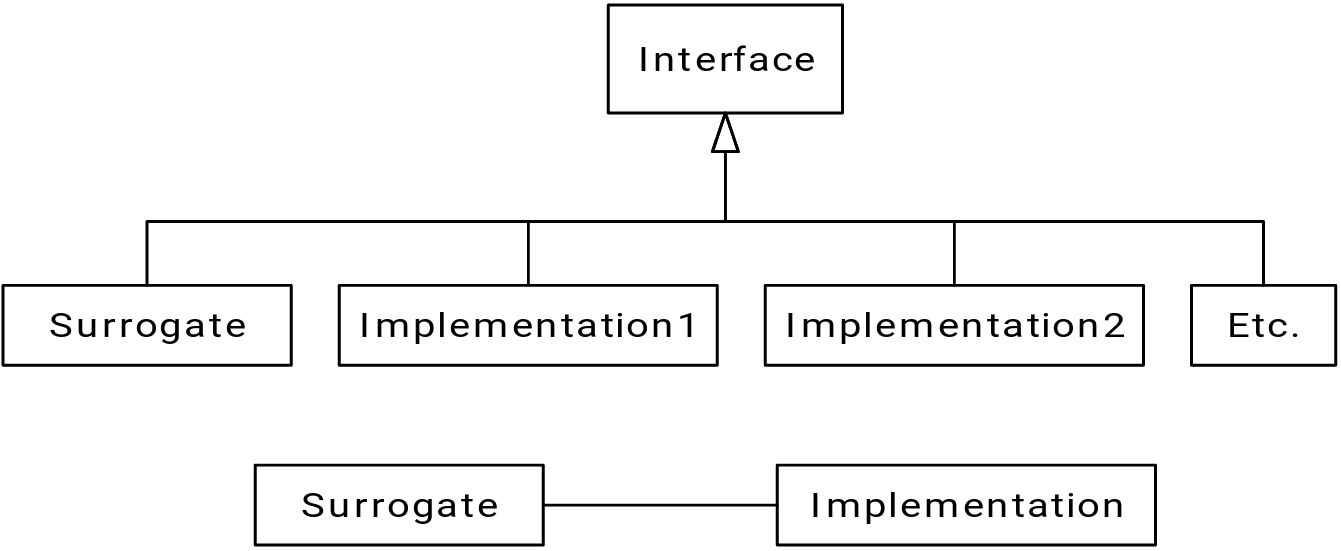
\includegraphics[width=\textwidth]{pg50} 
    \caption{tomado de: http://docs.linuxtone.org/ebooks/Python/Thinking\_In\_Python.pdf }
    \label{fig:mesh1}
\end{figure}

Cuando se crea un objeto sustituto, se da una implementación a la cual enviar todos los llamados a los métodos.    \newline

Estructuralmente, la diferencia entre \textit{Proxy} y \textit{State} es simple: un \textit{Proxy} tiene una sola implementación, mientras que \textit{State} tiene más de una implementación. La aplicación  de los patrones se considera en \textit{Design Patterns} (Patrones de Diseño) de forma distinta: \textit{Proxy} es usado para controlar el acceso a esta implementación, mientras \textit{State}  le permite cambiar la implementación de forma dinámica. Sin embargo, si expande su noción de "controlando el acceso a la implementación", entonces los dos encajan pulcramente juntos.

\subsection*{Proxy}
\label{subsec:Proxy}
\addcontentsline{toc}{subsection}{\nameref{subsec:Proxy}}

Si implementamos \textit{Proxy} siguiendo el diagrama anterior, se ve así:

 \begin{lstlisting} 
#: c04:ProxyDemo.py 
# Simple demonstration of the Proxy pattern. 

class Implementation: 
  def f(self):  
    print "Implementation.f()" 
  def g(self):  
    print "Implementation.g()"  
  def h(self):  
    print "Implementation.h()" 
    
class Proxy: 
  def __init__(self):  
    self.__implementation = Implementation()  
  # Pass method calls to the implementation: 
    def f(self): self.__implementation.f()  
  def g(self): self.__implementation.g()  
  def h(self): self.__implementation.h()  
  
p = Proxy() 
p.f(); p.g(); p.h() 
#:~ 
 \end{lstlisting}
 
No es necesario que \textbf{Implementation} tenga la misma interfaz que \textbf{Proxy}; siempre y cuando \textbf{Proxy} es de alguna manera \textit{ "speaking for"} ("hablando en nombre de") la clase se refiere a la llamada del método, para entonces la idea básica está satisfecha (tenga en cuenta que esta declaración está en contradicción con la definición de Proxy en GoF). Sin embargo, es conveniente tener una interfaz común para que \textbf{Implementation} se vea obligado a cumplir con todos los métodos que \textbf{Proxy} necesita llamar. \newline
	
Por supuesto, en Python tenemos un mecanismo de delegación integrado, lo que hace que el \textbf{Proxy} sea aún más simple de implementar:   \newline

\begin{lstlisting} 
#: c04:ProxyDemo2.py 
# Simple demonstration of the Proxy pattern. 

class Implementation2: 
  def f(self):  
    print "Implementation.f()" 
  def g(self):  
    print "Implementation.g()"  
  def h(self):  
    print "Implementation.h()" 
    
class Proxy2: 
  def __init__(self):  
    self.__implementation = Implementation2()  
  def __getattr__(self, name): 
    return getattr(self.__implementation, name) 
    
p = Proxy2() 
p.f(); p.g(); p.h(); 
#:~ 
\end{lstlisting}

La belleza de la utilización de  \textbf{\_\_getattr\_\_( )} es que \textbf{Proxy2} es completamente genérico, y no vinculada a cualquier implementación particular (en Java, un "proxy dinámico" bastante complicado ha sido creado para lograr esto mismo). 

\newpage

\subsection*{State}
\label{subsec:State}
\addcontentsline{toc}{subsection}{\nameref{subsec:State}}

El patrón \textit{State} añade más implementaciones a \textit{Proxy}, junto con una manera de cambiar de una implementación a otra durante tiempo de vida del sustituto: \newline

\begin{lstlisting} 
#: c04:StateDemo.py 
# Simple demonstration of the State pattern.

class State_d: 
  def __init__(self, imp):  
    self.__implementation = imp  
  def changeImp(self, newImp): 
    self.__implementation = newImp 
  # Delegate calls to the implementation: 
  def __getattr__(self, name): 
    return getattr(self.__implementation, name) 
    
class Implementation1: 
  def f(self):  
    print "Fiddle de dum, Fiddle de dee,"  
  def g(self):  
    print "Eric the half a bee."  
  def h(self):  
    print "Ho ho ho, tee hee hee,"  
    
class Implementation2: 
    def f(self):  
    print "We're Knights of the Round Table."  
  def g(self):  
    print "We dance whene'er we're able."  
  def h(self):  
    print "We do routines and chorus scenes"  
    
def run(b): 
  b.f() 
  b.g() 
  b.h() 
  b.g() 
  
b = State_d(Implementation1()) 
run(b) 
b.changeImp(Implementation2()) 
run(b) 
#:~ 
\end{lstlisting}

Se puede ver que la primera implementación se usa para una parte, a continuación, la segunda implementación se intercambia y se utiliza.     \newline

La diferencia entre \textit{Proxy} y \textit{State} está en los problemas que se resuelven. Los usos comunes para \textit{Proxy} como se describe en \textit{Design Patterns} son:

\begin{enumerate}[1.]

    \item \textbf{Proxy remoto.} Este proxy para un objeto en un espacio de dirección diferente. Se crea un proxy remoto de forma automática por el compilador RMI \textbf{rmic} ya que crea ramales y esqueletos.
    
    \item \textbf{Proxy virtual.} Esto proporciona "inicialización relajada" para crear objetos costosos por demanda.
    
    \item \textbf{Proxy de Protección.} Se usa cuando no se desea que el programador cliente tenga acceso completo a los objetos proxy.
    
    \item \textbf{Referencia inteligente.} Para agregar acciones adicionales cuando se accede al objeto proxy. Por ejemplo, o para llevar un registro del número de referencias que se realizan para un objeto en particular, con el fin de implementar el lenguaje \textit{copy-on-write} (copiar en escritura) y prevenir objeto aliasing.
    %Objeto aliasing   {sugerencias: objetos espejos}
    Un ejemplo sencillo es hacer el seguimiento del número de llamadas a un método en particular.
\end{enumerate}

Usted podría mirar una referencia de Python como un tipo de proxy de protección, ya que controla el acceso al objeto real de los demás (y asegura, por ejemplo, que no utilice una referencia nula). \newline

[[\textit{Proxy} y \textit{State} no son vistos como relacionados entre sí porque los dos se les da (lo que considero arbitrario) diferentes estructuras.
\textit{State}, en particular, utiliza una jerarquía de implementación separada pero esto me parece innecesario a menos que usted haya decidido que la implementación no está bajo su control (ciertamente una posibilidad, pero si usted es dueño de todo el código no parece haber ninguna razón para no beneficiarse de la elegancia y amabilidad de la clase base individual). En adición, \textit{Proxy} no necesita utilizar la misma clase base para su implementación, siempre y cuando el objeto proxy esté controlando el acceso al objetarlo "frente" a favor. %Corregir! 
Independientemente de los detalles, en ambos \textit{Proxy} y \textit{State} un sustituto está pasando la llamada al método a través de un objeto de implementación.]]

\newpage

\subsection*{StateMachine (Máquina de Estados)}
\label{subsec:sm}
\addcontentsline{toc}{subsection}{\nameref{subsec:sm}}


Mientras \textit{State} tiene una manera de permitir que el programador cliente cambie la implementación, \textit{StateMachine} impone una estructura para cambiar automáticamente la implementación de un objeto al siguiente. La implementación actual representa el estado en que un sistema está, y el sistema se comporta de manera diferente de un estado a otro (ya que utiliza \textit{State}). Basicamente, esta es una "state machine : máquina de estados" usando objetos.     \newline

El código que mueve el sistema de un estado a otro es a menudo un \textit{Template Method} (Método Plantilla), como se ve en el siguiente framework para una máquina de estados básica.    \newline

Cada estado puede estar en un \textbf{run( )} para cumplir con su comportamiento, y (en este diseño) también puede pasarlo a un objeto "input" y así puede decirle a que nuevo estado es removido basado en este "input".
La distinción clave entre este diseño y el siguiente es que aquí, cada objeto \textbf{State} decide lo que otros estados pueden avanzar, basado en "input”, mientras que en el posterior diseño de todas las transiciones de estado se llevan a cabo en una sola tabla. Otra forma de decirlo es que aquí, cada objeto \textbf{State} tiene su propia pequeña tabla \textbf{State}, y en el subsiguiente diseño hay una sola tabla directora de transición de estado para todo el sistema.   \newline

 \begin{lstlisting}
#: c04:statemachine:State.py 
# A State has an operation, and can be moved 
# into the next State given an Input: 

class State: 
  def run(self):  
    assert 1, "run not implemented" 
  def next(self, input): 
    assert 1, "next not implemented" 
#:~ 
 \end{lstlisting}
 
 Esta clase es claramente innecesaria, pero que nos permite decir que algo es un objeto \textbf{State} en el código, y proporcionar un mensaje de error ligeramente diferente cuando no se implementan todos los métodos. Podríamos haber conseguido básicamente el mismo efecto diciendo:      \newline
 
 \begin{lstlisting}
 class State: pass
 \end{lstlisting}
 
 Porque todavía conseguiríamos excepciones si \textbf{run} o \textbf{next()} hubieran sido llamados por un tipo derivado, y no hubieran sido implementados. \newline
 
El \textbf{StateMachine} hace un seguimiento de la situación actual, el cual es inicializado por el constructor. El método \textbf{runAll()} toma una lista de objetos \textbf{Input}. Este método no sólo avanza al siguiente estado, sino que también llama \textbf{run( )} para cada objeto \textit{state} – por lo tanto se puede ver que es una expansión de la idea del patrón \textbf{State}, ya que \textbf{run( )} hace algo diferente dependiendo del estado en que el sistema está.    \newline

\begin{lstlisting}
#: c04:statemachine:StateMachine.py 
# Takes a list of Inputs to move from State to  
# State using a template method. 

class StateMachine: 
  def __init__(self, initialState): 
    self.currentState = initialState 
    self.currentState.run() 
  # Template method: 
  def runAll(self, inputs): 
    for i in inputs: 
      print i 
      self.currentState = self.currentState.next(i) 
      self.currentState.run() 
#:~ 
\end{lstlisting}

También he tratado \textbf{runAll( )} como un método plantilla. Esto es típico, pero ciertamente no es necesario – posiblemente podría querer
%concievably == posiblemente
reemplazarlo, pero por lo general el cambio de comportamiento se producirá en \textbf{run( )} de \textbf{State} en su lugar.       \newline

En este punto se ha completado el framework básico para este estilo de StateMachine (donde cada estado decide los próximos estados). Como ejemplo, voy a utilizar una trampa de fantasía para que el ratón pueda moverse a través de varios estados en el proceso de atrapar un ratón\footnote{Ningún ratón fue perjudicado en la creación de este ejemplo.}. Las clases ratón y la información se almacenan en el paquete \textbf{mouse}, incluyendo una clase en representación de todas los posibles movimientos que un ratón puede hacer, que serán las entradas a la \textit{state machine} (máquina de estados):       \newline
% harm == dañar, perjudicar

\begin{lstlisting}
#: c04:mouse:MouseAction.py 

class MouseAction: 
  def __init__(self, action):  
    self.action = action 
  def __str__(self): return self.action  
  def __cmp__(self, other): 
    return cmp(self.action, other.action) 
  # Necessary when __cmp__ or __eq__ is defined 
  # in order to make this class usable as a 
  # dictionary key: 
  def __hash__(self):  
    return hash(self.action) 
    
# Static fields; an enumeration of instances: 
MouseAction.appears = MouseAction("mouse appears") 
MouseAction.runsAway = MouseAction("mouse runs away") 
MouseAction.enters = MouseAction("mouse enters trap") 
MouseAction.escapes = MouseAction("mouse escapes") 
MouseAction.trapped = MouseAction("mouse trapped") 
MouseAction.removed = MouseAction("mouse removed") 
#:~   
  \end{lstlisting}
  
Usted observará que \textbf{\_\_cmp\_\_( )} se ha reemplazado para implementar una comparación entre los valores de \textit{action}. También, cada posible movida de un ratón se enumera como un objeto de \textbf{MouseAction}, todos los cuales son los campos estáticos en \textbf{MouseAction}. \newline

Para la creación de código de prueba, una secuencia de entradas de mouse está provisto de un archivo de texto:  \newline
  
\begin{lstlisting}  
#:! c04:mouse:MouseMoves.txt 
mouse appears 
mouse runs away 
mouse appears 
mouse enters trap 
mouse escapes 
mouse appears 
mouse enters trap 
mouse trapped 
mouse removed 
mouse appears 
mouse runs away 
mouse appears 
mouse enters trap 
mouse trapped 
mouse removed 
#:~ 
\end{lstlisting}
 
 Con estas herramientas en su lugar, ahora es posible crear la primera versión del programa mousetrap (ratonera). Cada subclase \textbf{State} define su comportamiento \textbf{run( )} y también establece su siguiente estado con una sentencia \textbf{if-else}:   \newline
   
\begin{lstlisting}  
 #: c04:mousetrap1:MouseTrapTest.py 
# State Machine pattern using 'if' statements 
# to determine the next state. 
import string, sys 
sys.path += ['../statemachine', '../mouse'] 
from State import State 
from StateMachine import StateMachine 
from MouseAction import MouseAction 
# A different subclass for each state:

class Waiting(State): 
  def run(self):  
    print "Waiting: Broadcasting cheese smell" 
    
  def next(self, input): 
    if input == MouseAction.appears: 
      return MouseTrap.luring 
    return MouseTrap.waiting 
    
class Luring(State): 
  def run(self): 
    print "Luring:Presenting Cheese, door open" 
  def next(self, input): 
    if input == MouseAction.runsAway: 
      return MouseTrap.waiting 
    if input == MouseAction.enters: 
      return MouseTrap.trapping 
    return MouseTrap.luring 
    
class Trapping(State): 
  def run(self): 
    print "Trapping: Closing door"
    
  def next(self, input): 
    if input == MouseAction.escapes: 
      return MouseTrap.waiting 
    if input == MouseAction.trapped: 
      return MouseTrap.holding 
    return MouseTrap.trapping 
    
class Holding(State): 
  def run(self): 
    print "Holding: Mouse caught" 
   def next(self, input): 
    if input == MouseAction.removed: 
      return MouseTrap.waiting 
    return MouseTrap.holding 
    
class MouseTrap(StateMachine): 
  def __init__(self):  
    # Initial state 
    StateMachine.__init__(self, MouseTrap.waiting) 
    
# Static variable initialization: 
MouseTrap.waiting = Waiting() 
MouseTrap.luring = Luring() 
MouseTrap.trapping = Trapping() 
MouseTrap.holding = Holding() 

moves = map(string.strip,  
  open("../mouse/MouseMoves.txt").readlines()) 
MouseTrap().runAll(map(MouseAction, moves)) 
#:~ 
  \end{lstlisting}
  
  La clase \textbf{StateMachine} simplemente define todos los posibles estados como objetos estáticos, y también establece el estado inicial. \textbf{UnitTest} crea un \textbf{MouseTrap} y luego prueba con todas las entradas de un \textbf{MouseMoveList.}    \newline
  
  Mientras el uso de las sentencias \textbf{if} dentro de los métodos \textbf{next()} es perfectamente razonable, la gestión de un gran número de ellos podría llegar a ser difícil. Otro enfoque es crear tablas dentro de cada objeto \textbf{State} definiendo los diversos estados próximos basados en la entrada.    \newline
  
  Inicialmente, esto parece que debería ser bastante simple. Usted debe ser capaz de definir una tabla estática en cada subclase \textbf{State} que define las transiciones en términos de los otros objetos \textbf{State}. Sin embargo, resulta que este enfoque genera dependencias de inicialización cíclicas. Para resolver el problema, He tenido que retrasar la inicialización de las tablas hasta la primera vez que se llama al método  \textbf{next( )} para un objeto en particular \textbf{State}. Inicialmente, los métodos \textbf{next()} pueden parecer un poco extraños debido a esto.\newline
  
  La clase \textbf{StateT} es una implementación de \textbf{State} ((de modo que la misma clase \textbf{StateMachine} puede ser utilizado en el ejemplo anterior) que añade un \textbf{Map} y un método para inicializar el mapa a partir de una matriz de dos dimensiones. El "método \textbf{next()}" tiene una implementación de la clase base que debe ser llamado desde el "método \textbf{next()} de la clase derivada anulada", después de que se ponen a prueba para un \textbf{null Map} (y inicializarlo si es nulo):  \newline
  
 \begin{lstlisting}
#: c04:mousetrap2:MouseTrap2Test.py 
# A better mousetrap using tables 
import string, sys 
sys.path += ['../statemachine', '../mouse'] 
from State import State 
from StateMachine import StateMachine 
from MouseAction import MouseAction 

class StateT(State): 
  def __init__(self): 
    self.transitions = None 
  def next(self, input): 
    if self.transitions.has_key(input): 
      return self.transitions[input] 
    else: 
      raise "Input not supported for current state" 
class Waiting(StateT): 
  def run(self):  
    print "Waiting: Broadcasting cheese smell" 
  def next(self, input): 
    # Lazy initialization: 
    if not self.transitions: 
      self.transitions = {  
        MouseAction.appears : MouseTrap.luring  
      } 
    return StateT.next(self, input) 
class Luring(StateT): 
  def run(self): 
    print "Luring: Presenting Cheese, door open" 
  def next(self, input): 
    # Lazy initialization: 
    if not self.transitions: 
      self.transitions = { 
        MouseAction.enters : MouseTrap.trapping, 
        MouseAction.runsAway : MouseTrap.waiting 
      } 
    return StateT.next(self, input) 
class Trapping(StateT): 
  def run(self): 
  
      print "Trapping: Closing door" 
  def next(self, input): 
    # Lazy initialization: 
    if not self.transitions: 
      self.transitions = { 
        MouseAction.escapes : MouseTrap.waiting, 
        MouseAction.trapped : MouseTrap.holding 
      } 
    return StateT.next(self, input) 
class Holding(StateT): 
  def run(self): 
    print "Holding: Mouse caught" 
  def next(self, input): 
    # Lazy initialization: 
    if not self.transitions: 
      self.transitions = { 
        MouseAction.removed : MouseTrap.waiting 
      } 
    return StateT.next(self, input) 
class MouseTrap(StateMachine): 
  def __init__(self):  
    # Initial state 
    StateMachine.__init__(self, MouseTrap.waiting) 
# Static variable initialization: 
MouseTrap.waiting = Waiting() 
MouseTrap.luring = Luring() 
MouseTrap.trapping = Trapping() 
MouseTrap.holding = Holding() 
moves = map(string.strip,  
  open("../mouse/MouseMoves.txt").readlines()) 
mouseMoves = map(MouseAction, moves) 
MouseTrap().runAll(mouseMoves) 
#:~ 
 \end{lstlisting}
 
El resto del código es idéntico – la diferencia está en los métodos \textbf{next()} y la clase \textbf{StateT}.\newline

Si usted tiene que crear y mantener una gran cantidad de clases \textbf{State}, este enfoque es una mejora, ya que es más fácil de leer de forma rápida y comprender las transiciones de estado viendo la tabla.

\newpage

\subsection*{Table-Driven State Machine}
\label{subsec:tdsm}
\addcontentsline{toc}{subsection}{\nameref{subsec:tdsm}}

La ventaja del diseño anterior es que toda la información acerca de un estado, incluyendo la información de transición del estado,  se encuentra dentro de la misma clase \textit{state}. Esto es generalmente un buen principio de diseño.    \newline

Sin embargo, en una \textit{state machine} (máquina de estados) pura, la máquina puede ser completamente representada por una única tabla de transición de estados. Esto tiene la ventaja de localizar toda la información sobre la máquina de estados en un solo lugar, lo que significa que usted puede con mayor facilidad crear y mantener la tabla basada en un diagrama de transición de estados clásica.      \newline 

El diagrama clásico de transición de estados utiliza un círculo para representar cada estado, y las líneas del \textit{state} señalando a todos los estados en que \textit{state} puede trasladarse. Cada línea de transición se anota con condiciones para la transición y una acción durante la transición. El siguiente es su aspecto: \newline

(Diagrama State Machine simple) \newline

Objetivos:

\begin{itemize}
    \item Traducción directa del diagrama de estado
    \item Vector del cambio: la representación del diagrama de estado
    \item Implementación razonable
    \item No hay exceso de estados (usted podría representar a cada cambio individual con un nuevo estado)
    \item La simplicidad y la flexibilidad
\end{itemize}

Observaciones:

\begin{itemize}
    \item Los estados son triviales – ninguna información o funciones / datos, sólo una identidad.
    \item Diferente a \textit{State Pattern}!
    \item La máquina regula el paso de un estado a otro.
    \item Al igual que en flyweight : peso mosca
    \item Cada estado puede pasar a muchos otros
    \item Funciones de condición / acción también deben ser externos a los estados
    \item Centralizar la descripción en una sola tabla que contiene todas las variaciones, para facilitar la configuración.
\end{itemize}

Ejemplo:

\begin{itemize}
    \item State Machine y Table-Driven Code 
    \item Implementa una máquina expendedora
    \item Utiliza diferentes patrones
    \item Separa código común \textit{state-machine} de aplicaciones específicas (como método de plantilla)
    \item Cada entrada causa una búsqueda de la solución apropiada (como cadena de responsabilidad)
    \item Las pruebas y transiciones se encapsulan en objetos de funciones (objetos que contienen funciones)
    \item Restricción de Java: los métodos no son objetos de primera clase.
\end{itemize}

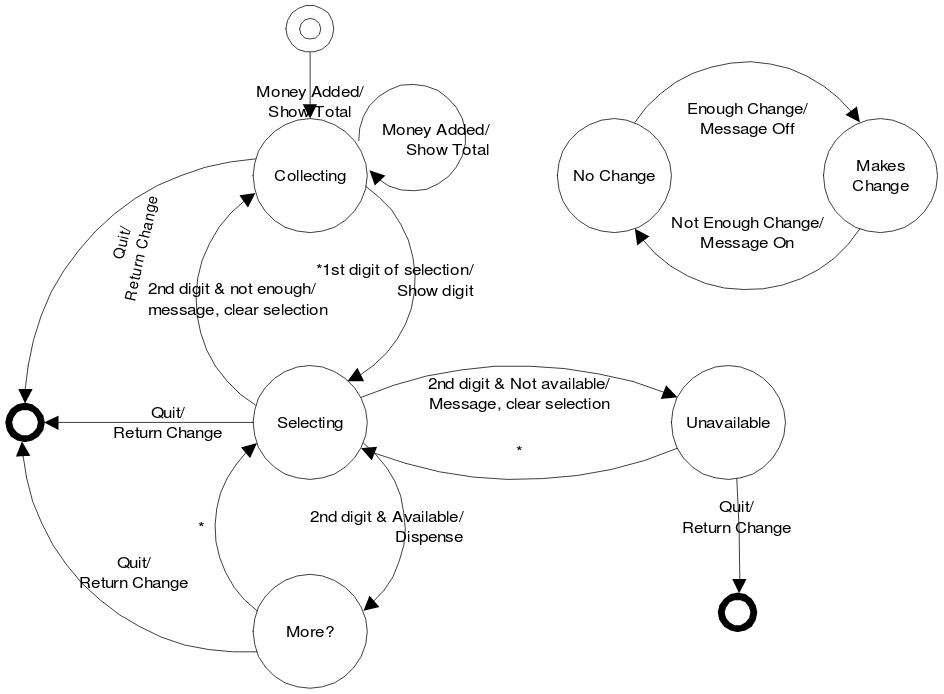
\includegraphics[width=\textwidth]{pag63}  


\subsubsection*{La clase State}
\label{subsubsec:lcs}
\addcontentsline{toc}{subsubsection}{\nameref{subsubsec:lcs}}

 La clase \textbf{State} es claramente diferente a la anterior, ya que es en realidad sólo un marcador de posición con un nombre. Por lo tanto, no se hereda de las clases \textbf{State} anteriores:    \newline
 
 \begin{lstlisting}
# c04:statemachine2:State.py 
class State: 
  def __init__(self, name): self.name = name 
  def __str__(self): return self.name  
# :~  
 \end{lstlisting}
  
  
\subsubsection*{Condiciones para la transición}
\label{subsubsec:cplt}
\addcontentsline{toc}{subsubsection}{\nameref{subsubsec:cplt}}  

En el diagrama de transición de estados, una entrada se pone a prueba para ver si satisface las condiciones necesarias para transferir al Estado en cuestión. Como antes, el \textbf{Input} es sólo una interfaz de etiquetado:     \newline

\begin{lstlisting}
# c04:statemachine2:Input.py 
# Inputs to a state machine 
class Input: pass 
# :~ 
\end{lstlisting}

La \textbf{Condition} evalúa el \textbf{Input} para decidir si esta fila en la tabla es la transición correcta: \newline

  \begin{lstlisting}
# c04:statemachine2:Condition.py 
# Condition function object for state machine 

class Condition: 
  boolean condition(input) :  
    assert 1, "condition() not implemented" 
# :~ 
\end{lstlisting}

\subsubsection*{Acciones de transición}
\label{subsubsec:adt}
\addcontentsline{toc}{subsubsection}{\nameref{subsubsec:adt}}


Si \textbf{Condition} devuelve \textbf{true}, entonces se hace la transición a un nuevo estado, y dado que esa transición se hace, algún tipo de acción ocurre (en el diseño anterior de \textit{state machine : máquina de estado}, éste era el método\textbf{run( )}).     \newline

\begin{lstlisting}
# c04:statemachine2:Transition.py 
# Transition function object for state machine 

class Transition: 
  def transition(self, input): 
    assert 1, "transition() not implemented" 
# :~ 
\end{lstlisting}

\subsubsection*{La tabla}
\label{subsubsec:lt}
\addcontentsline{toc}{subsubsection}{\nameref{subsubsec:lt}}

Con estas clases en el lugar, podemos establecer una tabla de 3 dimensiones, donde cada fila describe completamente un estado. El primer elemento en la fila es el estado actual, y el resto de los elementos de la fila, son los diferentes tipos de entradas posibles, la condición que se debe satisfacer para que este cambio de estado sea el correcto, la acción que ocurre durante la transición, y el nuevo estado al que se moverá dentro. Observe que el objeto \textbf{Input} no sólo se utiliza para su tipo, también es un objeto \textit{Messenger} que lleva la información a los objetos \textbf{Condition} y \textbf{ Transition} :     \newline

\begin{lstlisting}
{(CurrentState, InputA) : (ConditionA, TransitionA, NextA), 
 (CurrentState, InputB) : (ConditionB, TransitionB, NextB), 
 (CurrentState, InputC) : (ConditionC, TransitionC, NextC), 
 ... 
 }
\end{lstlisting}


\subsubsection*{La máquina básica}
\label{subsubsec:lmb}
\addcontentsline{toc}{subsubsection}{\nameref{subsubsec:lmb}}

\begin{lstlisting}
# c04:statemachine2:StateMachine.py 
# A table-driven state machine 

class StateMachine: 
  def __init__(self, initialState, tranTable): 
    self.state = initialState 
    self.transitionTable = tranTable 
    
  def nextState(self, input): 
  
    Iterator it=((List)map.get(state)).iterator() 
    while(it.hasNext()): 
      Object[] tran = (Object[])it.next() 
      if(input == tran[0] ||  
         input.getClass() == tran[0]): 
        if(tran[1] != null): 
          Condition c = (Condition)tran[1] 
          if(!c.condition(input)) 
            continue #Failed test
            
        if(tran[2] != null) 
          ((Transition)tran[2]).transition(input) 
        state = (State)tran[3] 
        return 
        
    throw RuntimeException( 
      "Input not supported for current state") 
      
# :~ 
\end{lstlisting}

\subsubsection*{Simple máquina expendedora}
\label{subsubsec:sme}
\addcontentsline{toc}{subsubsection}{\nameref{subsubsec:sme}}

\begin{lstlisting}
# c04:vendingmachine:VendingMachine.py 
# Demonstrates use of StateMachine.py 
import sys 
sys.path += ['../statemachine2'] 
import StateMachine 

class State: 
  def __init__(self, name): self.name = name 
  def __str__(self): return self.name  
State.quiescent = State("Quiesecent") 
State.collecting = State("Collecting") 
State.selecting = State("Selecting") 
State.unavailable = State("Unavailable") 
State.wantMore = State("Want More?") 
State.noChange = State("Use Exact Change Only") 
State.makesChange = State("Machine makes change") 

class HasChange: 
  def __init__(self, name): self.name = name 
  def __str__(self): return self.name  
  
HasChange.yes = HasChange("Has change") 
HasChange.no = HasChange("Cannot make change") 

class ChangeAvailable(StateMachine): 
  def __init__(self): 
    StateMachine.__init__(State.makesChange, { 
      # Current state, input 
      (State.makesChange, HasChange.no) : 
        # test, transition, next state: 
        (null, null, State.noChange), 
      (State.noChange, HasChange.yes) : 
        (null,null, State.noChange) 
    }) 
    
class Money: 
  def __init__(self, name, value): 
    self.name = name 
    self.value = value 
  def __str__(self): return self.name  
  def getValue(self): return self.value 
  
Money.quarter = Money("Quarter", 25) 
Money.dollar = Money("Dollar", 100) 

class Quit: 
  def __str__(self): return "Quit"  
  
Quit.quit = Quit() 

class Digit: 
  def __init__(self, name, value): 
    self.name = name 
    self.value = value 
  def __str__(self): return self.name  
  def getValue(self): return self.value  
  
class FirstDigit(Digit): pass 
FirstDigit.A = FirstDigit("A", 0) 
FirstDigit.B = FirstDigit("B", 1) 
FirstDigit.C = FirstDigit("C", 2) 
FirstDigit.D = FirstDigit("D", 3) 

class SecondDigit(Digit): pass 
SecondDigit.one = SecondDigit("one", 0) 
SecondDigit.two = SecondDigit("two", 1) 
SecondDigit.three = SecondDigit("three", 2) 
SecondDigit.four = SecondDigit("four", 3) 

class ItemSlot: 
  id = 0 
  def __init__(self, price, quantity): 
    self.price = price 
    self.quantity = quantity 
  def __str__(self): return `ItemSlot.id` 
  def getPrice(self): return self.price  
  def getQuantity(self): return self.quantity  
  def decrQuantity(self): self.quantity -= 1 
  
class VendingMachine(StateMachine): 
  changeAvailable = ChangeAvailable() 
  amount = 0 
  FirstDigit first = null 
  ItemSlot[][] items = ItemSlot[4][4] 
  
  # Conditions: 
  def notEnough(self, input): 
    i1 = first.getValue() 
    i2 = input.getValue() 
    return items[i1][i2].getPrice() > amount 
    
  def itemAvailable(self, input): 
    i1 = first.getValue() 
    i2 = input.getValue() 
    return items[i1][i2].getQuantity() > 0 
    
  def itemNotAvailable(self, input): 
    return !itemAvailable.condition(input) 
    #i1 = first.getValue() 
    #i2 = input.getValue() 
    #return items[i1][i2].getQuantity() == 0 
    
  # Transitions: 
  def clearSelection(self, input): 
    i1 = first.getValue() 
    i2 = input.getValue() 
    ItemSlot is = items[i1][i2] 
    print ( 
      "Clearing selection: item " + is + 
      " costs " + is.getPrice() + 
      " and has quantity " + is.getQuantity()) 
    first = null 
    
  def dispense(self, input): 
    i1 = first.getValue() 
    i2 = input.getValue() 
    ItemSlot is = items[i1][i2] 
    print ("Dispensing item " +  
      is + " costs " + is.getPrice() + 
      " and has quantity " + is.getQuantity()) 
    items[i1][i2].decrQuantity() 
    print ("Quantity " +  
      is.getQuantity()) 
    amount -= is.getPrice() 
    print("Amount remaining " +  
      amount) 
      
  def showTotal(self, input): 
    amount += ((Money)input).getValue() 
    print "Total amount = " + amount 
    
  def returnChange(self, input): 
    print "Returning " + amount 
    amount = 0 
    
  def showDigit(self, input): 
    first = (FirstDigit)input 
    print "First Digit= "+ first 
    
    
      def __init__(self): 
    StateMachine.__init__(self, State.quiescent) 
    for(int i = 0 i < items.length i++) 
      for(int j = 0 j < items[i].length j++) 
        items[i][j] = ItemSlot((j+1)*25, 5) 
    items[3][0] = ItemSlot(25, 0) 
    buildTable(Object[][][]{ 
     ::State.quiescent, # Current state 
        # Input, test, transition, next state: 
       :Money.class, null,  
         showTotal, State.collecting, 
     ::State.collecting, # Current state 
        # Input, test, transition, next state: 
       :Quit.quit, null,  
         returnChange, State.quiescent, 
       :Money.class, null,  
         showTotal, State.collecting, 
       :FirstDigit.class, null,  
         showDigit, State.selecting, 
     ::State.selecting, # Current state 
        # Input, test, transition, next state: 
       :Quit.quit, null,  
         returnChange, State.quiescent, 
       :SecondDigit.class, notEnough,  
         clearSelection, State.collecting, 
       :SecondDigit.class, itemNotAvailable,  
         clearSelection, State.unavailable, 
       :SecondDigit.class, itemAvailable,  
         dispense, State.wantMore, 
     ::State.unavailable, # Current state 
        # Input, test, transition, next state: 
       :Quit.quit, null,  
         returnChange, State.quiescent, 
       :FirstDigit.class, null,  
         showDigit, State.selecting, 
     ::State.wantMore, # Current state 
        # Input, test, transition, next state: 
       :Quit.quit, null,  
         returnChange, State.quiescent, 
       :FirstDigit.class, null,  
         showDigit, State.selecting, 
    ) 
    # :~ 
\end{lstlisting}

\subsubsection*{Prueba de la máquina}
\label{subsubsec:pdlm}
\addcontentsline{toc}{subsubsection}{\nameref{subsubsec:pdlm}}


\begin{lstlisting} 
# c04:vendingmachine:VendingMachineTest.py 
# Demonstrates use of StateMachine.py 

vm = VendingMachine() 
for input in [   
    Money.quarter, 
    Money.quarter, 
    Money.dollar, 
    FirstDigit.A, 
    SecondDigit.two, 
    FirstDigit.A, 
    SecondDigit.two, 
    FirstDigit.C, 
    SecondDigit.three, 
    FirstDigit.D, 
    SecondDigit.one, 
    Quit.quit]: 
  vm.nextState(input) 
# :~ 
\end{lstlisting}


\subsection*{Herramientas}
\label{subsec:Herramientas}
\addcontentsline{toc}{subsection}{\nameref{subsec:Herramientas}}

Otro enfoque, ya que su \textit{state machine} (máquina de estado) se hace más grande, es el uso de una herramienta de automatización mediante el cual se configura una tabla y se deja que la herramienta genere el código state machine para usted. Esto puede ser creado por sí mismo utilizando un lenguaje como Python, pero también hay herramientas libres de código abierto como \textit{Libero}, en \url{http://www.imatix.com/} \newline 


\subsection*{Ejercicios}
\label{subsec:Ejercicios}
\addcontentsline{toc}{subsection}{\nameref{subsec:Ejercicios}}

1. Crear un ejemplo del "proxy virtual". \newline

2. Crear un ejemplo del proxy "Referencia Inteligente" donde se guarda la cuenta del número de llamadas a los métodos y a un objeto en particular. \newline

3. Crear un programa similar a ciertos sistemas DBMS (Sistema Manejador de Bases de Datos) que sólo permiten un cierto número de conexiones en cualquier momento. Para implementar esto, utilizar 'Singleton' como un sistema que controla el número de objetos "connections" que se crean. Cuando un usuario ha terminado con una conexión, el sistema debe ser informado de manera que pueda comprobar que la conexión volverá a ser reutilizada. Para garantizar esto, proporcionar un objeto proxy en lugar de una referencia a la conexión actual, y diseñar el proxy de manera que haga que la conexión a ser liberada regrese al sistema.   \newline

4. Usando \textit{State}, hacer una clase llamada \textbf{UnpredictablePerson} que cambia el tipo de respuesta a su método \textbf{hello( )} dependiendo de qué tipo de \textbf{Mood} está adentro. Añada un tipo de clase adicional \textbf{Mood} llamada \textbf{Prozac}.  \newline

5. Cree una copia simple en la implementación de escritura.   \newline

6. Aplicar \textbf{TransitionTable.py} al problema "Washer : Lavadora"  \newline

7. Crear un sistema \textit{StateMachine} mediante el cual el estado actual junto con la información de entrada determina el siguiente estado en que el sistema estará. Para hacer esto, cada estado debe almacenar una referencia de nuevo al objeto proxy (el controlador de estado) de modo que pueda solicitar el cambio de estado. Use un \textbf{HashMap} para crear una tabla de estados, donde la clave es un \textbf{String} que nombre el nuevo estado y el valor es el nuevo estado del objeto. Dentro de cada subclase \textbf{state} reemplazar un método \textbf{nextState( )} que tiene su propia tabla de transición de estados. La entrada a \textbf{nextState( )} debe ser una sola palabra que sale de un archivo de texto que contiene una palabra por línea.  \newline

8. Modificar el ejercicio anterior para que la \textbf{state machine} pueda ser configurada mediante la creación / modificación de una sola matriz multidimensional. \newline

9- Modificar el ejercicio  "mood” de la sesión anterior para que se convierta en una  \textbf{state machine} (máquina de estado) usando StateMachine.java     \newline

10. Crear un sistema elevador de \textbf{state machine} utilizando StateMachine.java     \newline

11. Crear un sistema de calefacción / aire acondicionado usando StateMachine.java   \newline

12. Un \textit{generator}(generador) es un objeto que produce otros objetos, al igual que una fábrica, excepto que la función generador no requiere ningún argumento. Cree un \textbf{MouseMoveGenerator} que produce acciones correctas \textbf{MouseMove} como salidas cada vez que la función generador es llamada (es decir, el mouse debe moverse en la secuencia apropiada, por lo que los movimientos posibles se basan en el movimiento anterior – esto es otra state machine). Agregue un método \textbf{iterator( )} para producir un iterador, pero este método debe tomar un argumento  \textbf{int} que especifica el número de movimientos a producir antes de \textbf{hasNext( )} que retorna \textbf{false}.
        % Al frente de una implementación

\section*{\texorpdfstring{X: Decoradores: \newline  Selección de tipo dinámico}{X: Decoradores:  Selección Tipo dinámico}}
\label{sec:xdstd}
\addcontentsline{toc}{section}{\nameref{sec:xdstd}}


\textbf{El uso de objetos en capas, para añadir de forma dinámica y transparente, responsabilidades a los objetos individuales se le conoce como el patrón \textit{decorator} (decorador)}. \newline

Se utilizan cuando la subclasificación crea demasiadas (o inflexibles) clases.   \newline

Todos los decoradores que envuelven al objeto original deben tener la misma interfaz básica. \newline

Dynamic proxy/surrogate? (¿Proxy dinámico/subrogado?)  \newline

Esto explica la estructura de herencia singular.    \newline

Tradeoff:  la codificación es más complicado cuando se utiliza decoradores.

\newpage

\subsection*{Estructura Decorador básico}
\label{subsec:edb}
\addcontentsline{toc}{subsection}{\nameref{subsec:edb}}

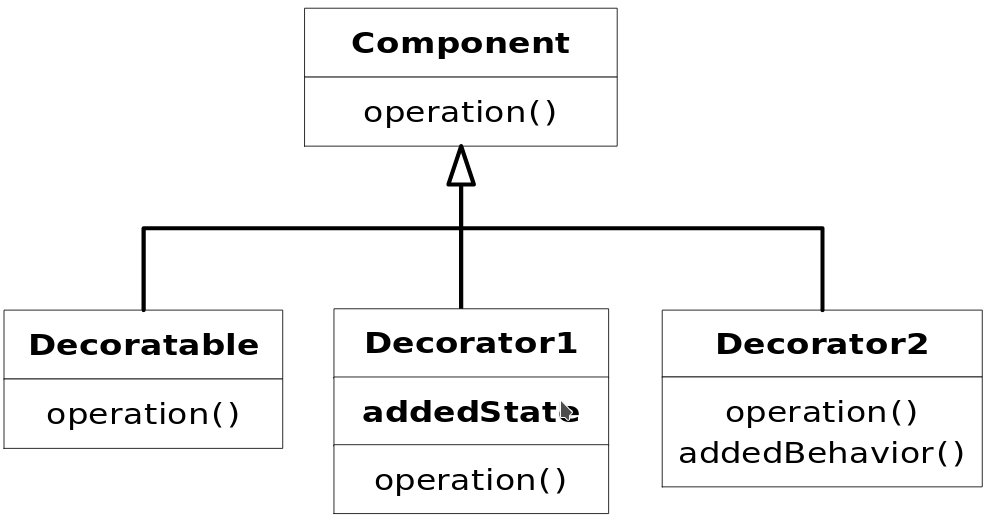
\includegraphics[width=\textwidth]{Pag73}

\subsection*{Un ejemplo café}
\label{subsec:uec}
\addcontentsline{toc}{subsection}{\nameref{subsec:uec}}

Considere la posibilidad de bajar a la cafetería local, \textit{BeanMeUp}, por un café. Normalmente hay muchas bebidas diferentes que se ofrecen \-\- expresos, cafés con leche, tés, cafés helados, chocolate caliente para nombrar unos pocos, así como una serie de extras (que cuestan extra también), tales como la crema batida o una inyección extra de expreso. Usted también puede hacer ciertos cambios en su bebida, sin costo adicional, como pedir café descafeinado en lugar de café regular.     \newline

Con bastante claridad si vamos a modelar todas estas bebidas y combinaciones, habrá diagramas de clases de tamaño variable. Así que para mayor claridad nosotros sólo consideraremos un subconjunto de los cafés: Expreso, café vienés, Caffe Latte,
Cappuccino y Café Mocha. 
Incluiremos 2 extras - crema batida ("batida") y una inyección extra de café expreso; y tres cambios - descafeinado, leche al vapor ("húmeda") y espuma de leche ("seco").   \newline

\subsection*{Clase para cada combinación}
\label{subsec:cpcc}
\addcontentsline{toc}{subsection}{\nameref{subsec:cpcc}}

Una solución es crear una clase individual  para cada combinación.Cada clase describe la bebida y es responsable por el costo, etc. El menú resultante es enorme, y una parte del diagrama de clases sería algo como esto:    \newline

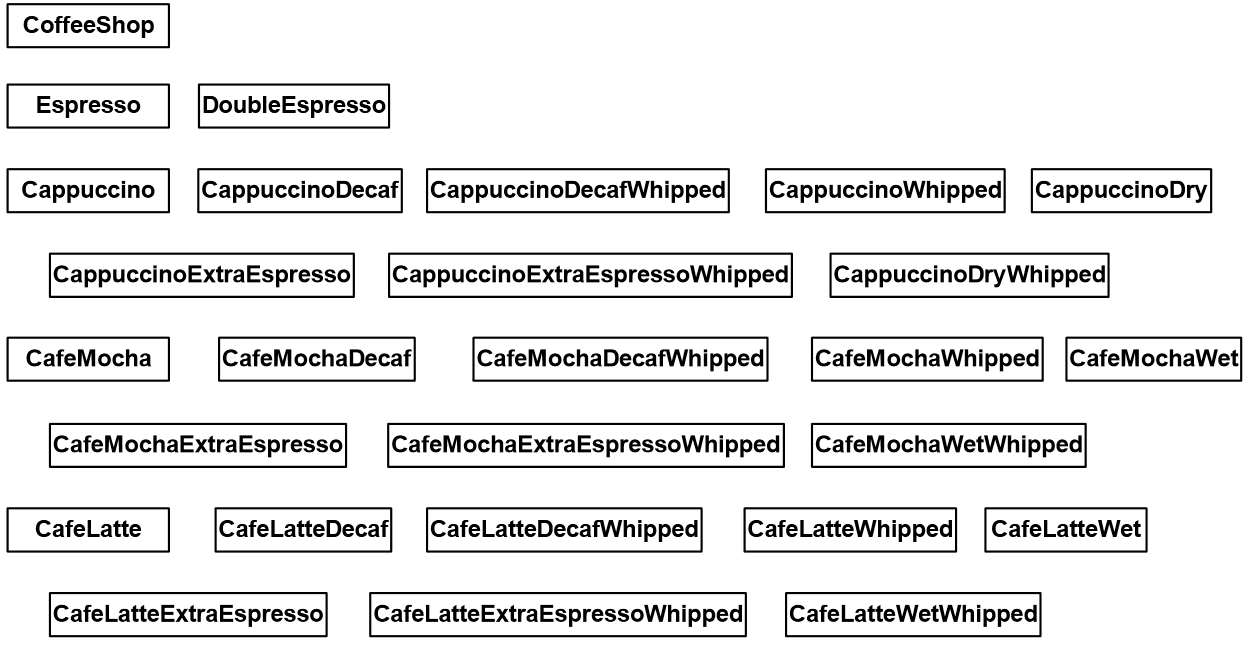
\includegraphics[width=\textwidth]{PaginaNo74} 

Aqui esta una de las combinaciones, una implementación simple de un Cappuccino:     \newline

\begin{lstlisting} 
class Cappuccino: 
  def __init__(self): 
    self.cost = 1 
    self.description = "Cappucino" 
  def getCost(self): 
    return self.cost 
  def getDescription(self): 
    return self.description 
\end{lstlisting}

La clave para el uso de este método es encontrar la combinación particular que desea. Así, una vez que haya encontrado la bebida que le gustaría, aquí le presentamos una forma de hacerlo, como se muestra en la clase \textbf{CoffeeShop} en el siguiente código:     \newline

\begin{lstlisting}
#: cX:decorator:nodecorators:CoffeeShop.py 
# Coffee example with no decorators 

class Espresso: pass 
class DoubleEspresso: pass

class EspressoConPanna: pass 

class Cappuccino: 
  def __init__(self): 
    self.cost = 1 
    self.description = "Cappucino" 
  def getCost(self): 
    return self.cost 
  def getDescription(self): 
    return self.description 
    
class CappuccinoDecaf: pass 
class CappuccinoDecafWhipped: pass 
class CappuccinoDry: pass 
class CappuccinoDryWhipped: pass 
class CappuccinoExtraEspresso: pass 
class CappuccinoExtraEspressoWhipped: pass 
class CappuccinoWhipped: pass 

class CafeMocha: pass 
class CafeMochaDecaf: pass 
class CafeMochaDecafWhipped: 
  def __init__(self): 
    self.cost = 1.25 
    self.description = \ 
      "Cafe Mocha decaf whipped cream" 
  def getCost(self): 
    return self.cost 
  def getDescription(self): 
    return self.description 
    
class CafeMochaExtraEspresso: pass 
class CafeMochaExtraEspressoWhipped: pass 
class CafeMochaWet: pass 
class CafeMochaWetWhipped: pass 
class CafeMochaWhipped: pass 

class CafeLatte: pass 
class CafeLatteDecaf: pass 
class CafeLatteDecafWhipped: pass 
class CafeLatteExtraEspresso: pass 
class CafeLatteExtraEspressoWhipped: pass 
class CafeLatteWet: pass 
class CafeLatteWetWhipped: pass 

class CafeLatteWhipped: pass 
cappuccino = Cappuccino() 
print (cappuccino.getDescription() + ": \$" +  
  `cappuccino.getCost()`) 
  
cafeMocha = CafeMochaDecafWhipped() 
print (cafeMocha.getDescription() 
  + ": \$" + `cafeMocha.getCost()`) 
#:~ 
\end{lstlisting}

y aquí está la salida correspondiente: \newline

\begin{lstlisting} 
Cappucino: $1.0Cafe Mocha decaf whipped cream: $1.25
\end{lstlisting}

Se puede ver que la creación de la combinación particular que se desea es fácil, ya que sólo está creando una instancia de una clase. Sin embargo, hay una serie de problemas con este enfoque. En primer lugar, las combinaciones son fijadas estáticamente para que cualquier combinación de un cliente que, quizá desee ordenar, necesite ser creada por adelantado. En segundo lugar, el menú resultante es tan grande que la búsqueda de su combinación particular es difícil y consume mucho tiempo.     \newline


\subsection*{El enfoque decorador}
\label{subsec:eed}
\addcontentsline{toc}{subsection}{\nameref{subsec:eed}}

Otro enfoque sería descomponer las bebidas en los diversos componentes, tales como expreso y leche espumada, y luego dejar que el cliente combine los componentes para describir un café en particular.    \newline

Con el fin de hacer esto mediante programación, utilizamos el patrón Decorador. Un decorador añade la responsabilidad de un componente envolviéndolo, pero el decorador se ajusta a la interfaz del componente que encierra, por lo que la envoltura es transparente. Los Decoradores también se pueden anidar sin la pérdida de esta transparencia. \newline

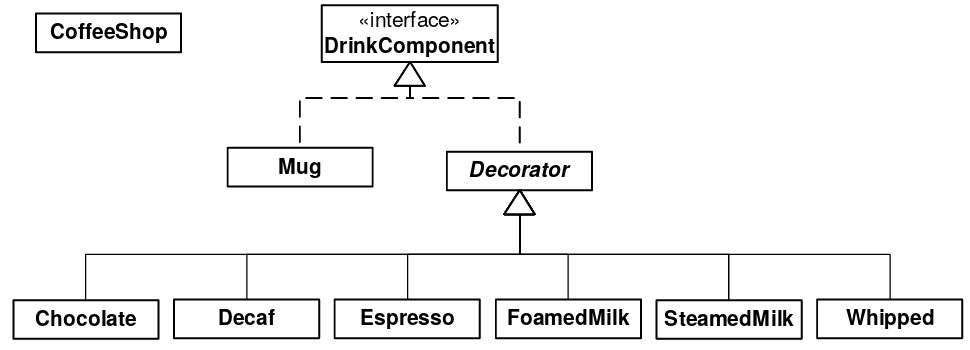
\includegraphics[width=\textwidth]{Pag77}

Métodos invocados en el Decorador a su vez pueden invocar métodos en el componente, y puede realizar, por supuesto, el procesamiento antes o después de la invocación.   \newline

Así que si añadimos los métodos \textbf{getTotalCost()} y \textbf{getDescription()} a la interfaz \textbf{DrinkComponent}, un Espresso se ve así:     \newline

\begin{lstlisting} 
class Espresso(Decorator): 
  cost = 0.75f 
  description = " espresso" 
  public Espresso(DrinkComponent): 
    Decorator.__init__(self, component) 
    
  def getTotalCost(self): 
    return self.component.getTotalCost() + cost 
    
  def getDescription(self): 
    return self.component.getDescription() + 
      description 
\end{lstlisting}

Usted combina los componentes para crear una bebida de la siguiente manera, como se muestra en el siguiente código:     \newline

\begin{lstlisting} 
#: cX:decorator:alldecorators:CoffeeShop.py 
# Coffee example using decorators

class DrinkComponent: 
  def getDescription(self): 
    return self.__class__.__name__ 
  def getTotalCost(self): 
    return self.__class__.cost 
    
class Mug(DrinkComponent): 
  cost = 0.0 
  
class Decorator(DrinkComponent): 
  def __init__(self, drinkComponent): 
    self.component = drinkComponent 
  def getTotalCost(self): 
    return self.component.getTotalCost() + \ 
      DrinkComponent.getTotalCost(self) 
  def getDescription(self): 
    return self.component.getDescription() + \ 
      ' ' + DrinkComponent.getDescription(self) 
      
class Espresso(Decorator): 
  cost = 0.75 
  def __init__(self, drinkComponent): 
    Decorator.__init__(self, drinkComponent) 
    
class Decaf(Decorator): 
  cost = 0.0 
  def __init__(self, drinkComponent): 
    Decorator.__init__(self, drinkComponent) 
    
class FoamedMilk(Decorator): 
  cost = 0.25 
  def __init__(self, drinkComponent): 
    Decorator.__init__(self, drinkComponent) 
    
class SteamedMilk(Decorator): 
  cost = 0.25 
    def __init__(self, drinkComponent): 
    Decorator.__init__(self, drinkComponent) 
class Whipped(Decorator): 
  cost = 0.25 
  def __init__(self, drinkComponent): 
    Decorator.__init__(self, drinkComponent) 
class Chocolate(Decorator): 
  cost = 0.25 
  def __init__(self, drinkComponent): 
    Decorator.__init__(self, drinkComponent) 
cappuccino = Espresso(FoamedMilk(Mug())) 
print cappuccino.getDescription().strip() + \ 
  ": \$" + `cappuccino.getTotalCost()`
  
cafeMocha = Espresso(SteamedMilk(Chocolate( 
  Whipped(Decaf(Mug()))))) 
  
print cafeMocha.getDescription().strip() + \ 
  ": \$" + `cafeMocha.getTotalCost()` 
#:~ 
\end{lstlisting}

Este enfoque, sin duda, proporciona la mayor flexibilidad y el menú más pequeño. Usted tiene un pequeño número de componentes para elegir,  pero el montaje de la descripción del café entonces se vuelve bastante arduo.   \newline

Si quiere describir un capuchino sencillo, se crea con \newline

\begin{lstlisting} 
plainCap = Espresso(FoamedMilk(Mug()))
\end{lstlisting}

Creando un Café Mocha descafeinado con crema batida requiere una descripción aún más larga. \newline


\subsection*{Compromiso}
\label{subsec:c}
\addcontentsline{toc}{subsection}{\nameref{subsec:c}}

El enfoque anterior toma demasiado tiempo para describir un café. También habrá ciertas combinaciones que se irán describiendo de manera regular, y sería conveniente tener una forma rápida de describirlos.     \newline

El tercer enfoque es una mezcla de los 2 primeros enfoques, y combina flexibilidad con la facilidad de uso. Este compromiso se logra mediante la creación de un menú de tamaño razonable de opciones básicas, que a menudo funcionan exactamente como son, pero si quería decorarlos (crema batida, descafeinado etc), entonces usted usaría decoradores para hacer las modificaciones. Este es el tipo de menú que se le presenta en la mayoría de tiendas de café.    \newline

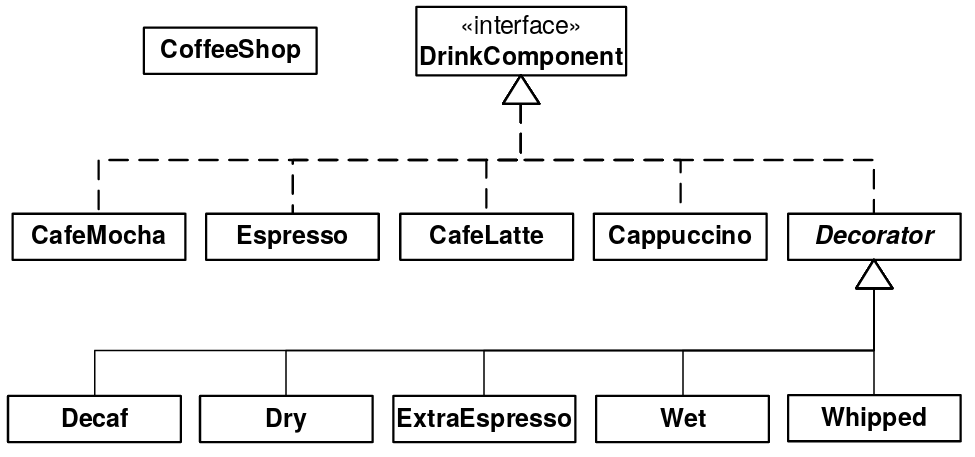
\includegraphics[width=\textwidth]{Pag80}

Se muestra cómo crear una selección básica, así como una selección decorada:     \newline

\begin{lstlisting} 
#: cX:decorator:compromise:CoffeeShop.py 
# Coffee example with a compromise of basic 
# combinations and decorators 

class DrinkComponent: 
  def getDescription(self): 
    return self.__class__.__name__ 
  def getTotalCost(self): 
    return self.__class__.cost 
    
class Espresso(DrinkComponent): 
  cost = 0.75 
  
class EspressoConPanna(DrinkComponent): 
  cost = 1.0 
  
class Cappuccino(DrinkComponent): 
  cost = 1.0 
  
class CafeLatte(DrinkComponent): 
  cost = 1.0 
  
class CafeMocha(DrinkComponent): 
  cost = 1.25 
  
class Decorator(DrinkComponent): 
  def __init__(self, drinkComponent): 
    self.component = drinkComponent 
  def getTotalCost(self): 
      return self.component.getTotalCost() + \ 
      DrinkComponent.getTotalCost(self) 
  def getDescription(self): 
    return self.component.getDescription() + \ 
      ' ' + DrinkComponent.getDescription(self) 
      
class ExtraEspresso(Decorator): 
  cost = 0.75 
  def __init__(self, drinkComponent): 
    Decorator.__init__(self, drinkComponent) 
    
class Whipped(Decorator): 
  cost = 0.50 
  def __init__(self, drinkComponent): 
    Decorator.__init__(self, drinkComponent) 
    
class Decaf(Decorator): 
  cost = 0.0 
  def __init__(self, drinkComponent): 
    Decorator.__init__(self, drinkComponent) 
    
class Dry(Decorator): 
      cost = 0.0 
  def __init__(self, drinkComponent): 
    Decorator.__init__(self, drinkComponent) 
    
class Wet(Decorator): 
  cost = 0.0 
  def __init__(self, drinkComponent): 
    Decorator.__init__(self, drinkComponent) 
    
cappuccino = Cappuccino() 
print cappuccino.getDescription() + ": \$" + \ 
  `cappuccino.getTotalCost()` 
  
cafeMocha = Whipped(Decaf(CafeMocha())) 
print cafeMocha.getDescription() + ": \$" + \ 
  `cafeMocha.getTotalCost()` 
#:~ 
\end{lstlisting}

Usted puede ver que creando una selección básica es rápido y fácil, lo cual tiene sentido ya que serán descritos con regularidad. Describiendo una bebida decorada hay más trabajo que cuando se utiliza una clase por combinación, pero claramente menos trabajo que cuando se usan solo los decoradores.    \newline

El resultado final no es demasiadas clases, ni tampoco demasiados decoradores. La mayoría de las veces es posible alejarse sin utilizar ningún decorador en absoluto, así tenemos los beneficios de ambos enfoques.     \newline


\subsection*{Otras consideraciones}
\label{subsec:oc}
\addcontentsline{toc}{subsection}{\nameref{subsec:oc}}


¿Qué sucede si decidimos cambiar el menú en una etapa posterior, tal como mediante la adición de un nuevo tipo de bebida? Si hubiéramos utilizado la clase por enfoque de combinación, el efecto de la adición de un ejemplo adicional como Syrup sería un crecimiento exponencial en el número de clases. Sin embargo, las implicaciones para todos los enfoques decorador o de compromiso son los mismos \- , se crea una clase extra.    \newline

¿Qué tal el efecto de cambiar el costo de la leche al vapor y espuma de leche, cuando el precio de la leche sube? Teniendo una clase para cada combinación significa que usted necesita cambiar un método en cada clase, y así mantener muchas clases. Mediante el uso de decoradores, el mantenimiento se reduce mediante la definición de la lógica en un solo lugar.  \newline

\subsection*{Ejercicios}
\label{subsec:ejer}
\addcontentsline{toc}{subsection}{\nameref{subsec:ejer}}

\begin{enumerate}[1.]
    \item Añadir una clase Syrup al enfoque decorador descrito anteriormente. A continuación, cree un Café Latte (usted necesitará usar la leche al vapor con un expreso) con Syrup.
    \item Repita el ejercicio 1 para el enfoque de compromiso.
    \item Implementar el patrón decorador para crear un restaurante de Pizza, el cual tenga un menú de opciones, así como la opción de diseñar su propia pizza. Siga el enfoque de compromiso para crear un menú que consiste en una margherita, hawaianas, regina, y pizzas vegetarianas, con relleno (decoradores) de ajo, aceitunas, espinacas, aguacate, queso feta y Pepperdews. Crear una pizza hawaiana, así como un Margherita decorado con espinacas, queso feta, Pepperdews y aceitunas.
\end{enumerate}

\newpage
       % X: Decoradores: Selección Tipo dinámico

\section*{\texorpdfstring{Y: Iteradores: \newline  Algoritmos de desacoplamiento de contenedores}{Y: Iteradores: Algoritmos de desacoplamiento de contenedores}}
\label{sec:yiadddc}
\addcontentsline{toc}{section}{\nameref{sec:yiadddc}}


\textit{Alexander Stepanov pensó durante años sobre el problema de las técnicas de programación genéricas antes de crear el STL (Standard Template Library) (junto con Dave Musser). Llegó a la conclusión de que todos los algoritmos están definidos en las estructuras algebraicas – lo que llamaríamos contenedores.}

En el proceso, Alexander Stepanov se dio cuenta que los iteradores son fundamentales para el uso de algoritmos, porque desacoplan los algoritmos del tipo especifico de contenedor con que el algoritmo actualmente podría estar trabajando. Esto significa que usted puede describir el algoritmo sin preocuparse de la secuencia particular en la cual está operando. En general, \textit{cualquier} código que usted escribe utilizando iteradores es desacoplado de la estructura de datos que el código está manipulando, y por lo tanto su código es más general y reutilizable. \newline

El uso de iteradores también amplía su código en el campo de \textit{programación funcional}, cuyo objetivo es describir lo que un programa está haciendo a cada paso en lugar de cómo lo está haciendo. Es decir, usted dice "el tipo" en lugar de describir el tipo. El objetivo del STL de C ++ era proporcionar este enfoque a la programación genérica de C ++ (cómo el éxito de este enfoque será en la realidad, aún está por verse). \newline

Si ha utilizado contenedores en Java (y es difícil escribir código sin usarlos), ha utilizado iteradores – en forma del \textbf{Enumeration} en Java 1.0/1.1 y de \textbf{Iterator} en Java 2.0. Así que usted ya debe estar familiarizado con su uso general.\footnote{Si no, consulte el Capítulo 9, \textit{Holding Your Objects  (Manteniendo Sus objetos)}, en \textit{Iterators in Thinking in Java} segunda edición (descargable gratuitamente desde \url{www.bruceeckel.com/}).} \newline

Debido a que en Java 2.0 los contenedores dependen en gran medida de los iteradores, se convierten en excelentes candidatos para las técnicas de programación genéricas / funcionales. Este capítulo explorará estas técnicas mediante la conversión de los algoritmos de STL para Java, para su uso con la librería de contenedor Java 2.  \newline


\subsection*{Iteradores Type-safe}
\label{subsec:icsdt}
\addcontentsline{toc}{subsection}{\nameref{subsec:icsdt}}


En \textit{Thinking in Java, segunda edición}, muestro la creación de un contenedor Type-safe que sólo aceptará un tipo particular de objeto. Un lector, Linda Pazzaglia, preguntó por el otro componente obvio type-safe, un iterador que trabajaría con los contenedores básicos \textbf{java.util}, pero imponer la restricción de que el tipo de objetos sobre los que itera sea de un tipo particular. \newline

Si Java siempre incluye un mecanismo de plantilla, este tipo de iterador tendrá la ventaja añadida de ser capaz de devolver un tipo específico de objeto, pero sin las plantillas se ve obligado a retornar \textbf{Objects} genéricos, o requerir un poco de codificación manual para cada tipo que desea iterar. Tomaré el enfoque anterior.     \newline

Una segunda decisión de diseño involucra el tiempo en que se determina el tipo de objeto. Un enfoque consiste en tomar el tipo del primer objeto que el iterador encuentra, pero esto es problemático debido a que los contenedores pueden arreglar de nuevo los objetos de acuerdo con un mecanismo de ordenamiento interno (tal como una tabla hash) y por lo tanto es posible obtener diferentes resultados de una iteración a la siguiente. El enfoque seguro es exigir al usuario establecer el tipo durante la construcción del iterador.     \newline

Por último, ¿cómo construir el iterador? No podemos reescribir las librerías de clases Java existentes que ya producen \textbf{Enumerations} e \textbf{Iterators}.  Sin embargo, podemos utilizar el patrón de diseño \textit{Decorator}, y crear una clase que simplemente envuelve el \textbf{Enumeration} o \textbf{Iterator} que se produce, generando un nuevo objeto que tiene el comportamiento de iteración que queremos (que es, en este caso, lanzar un \textbf{RuntimeException} si se encuentra un tipo incorrecto) pero con la misma interfaz que el \textbf{Enumeration} original o \textbf{Iterator}, de modo que se puede utilizar en los mismos lugares (puede argumentar que esto es en realidad un patrón \textit{Proxy}, pero es más probable \textit{Decorator} debido a su intención). Aquí está el código: \newline

\begin{lstlisting} 
# util:TypedIterator.py 

class TypedIterator(Iterator): 
  private Iterator imp 
  private Class type 
  def __init__(self, Iterator it, Class type): 
    imp = it 
    self.type = type 
    
  def hasNext(self):  
    return imp.hasNext()  
    
  def remove(self): imp.remove()  
  def next(self): 
    Object obj = imp.next() 
    if(!type.isInstance(obj)) 
      throw ClassCastException( 
        "TypedIterator for type " + type + 
        " encountered type: " + obj.getClass()) 
    return obj 
# :~ 
\end{lstlisting}
      % Y: Iteradores: Algoritmos de desacoplamiento de contenedores

\section*{\texorpdfstring{5: Fábricas: \newline  encapsular \newline la creación de objetos}{5: Fábricas: encapsular la creación de objetos}}
\label{sec:felcdo}
\addcontentsline{toc}{section}{\nameref{sec:felcdo}}

%\section{5: Fábricas: \newline  encapsular \newline la creación de objetos}

Cuando descubre que es necesario agregar nuevos tipos a un sistema, el primer paso más sensato es utilizar el polimorfismo para crear una interfaz común a esos nuevos tipos. Esto separa el resto del código en el sistema desde el conocimiento de los tipos específicos que está agregando. Nuevos tipos pueden añadirse sin molestar código existente ... o al menos eso parece. Al principio parecería que el único lugar que necesita cambiar el código en tal diseño es el lugar donde usted hereda un nuevo tipo, pero esto no es del todo cierto. Usted todavía debe crear un objeto de su nuevo tipo, y en el punto de la creación debe especificar el constructor exacto a utilizar. Así, si el código que crea objetos se distribuye a través de su aplicación, usted tiene el mismo problema cuando añade nuevos tipos — usted todavía debe perseguir todos los puntos de su código en asuntos de tipos. Esto sucede para ser la \textit{creation : creación} del tipo que importa en este caso en lugar del \textit{use : uso} del tipo (que es atendido por el polimorfismo), pero el efecto es el mismo : la adición de un nuevo tipo puede causar problemas. \newline

La solución es forzar la creación de objetos que se produzca a través de una \textit{factory : fábrica} común antes que permitir que el código creacional que se extendió por todo el sistema. Si todo el código en su programa debe ir a través de esta fábrica cada vez que necesita crear uno de sus objetos, entonces todo lo que debe hacer cuando añada un nuevo objeto es modificar la fábrica.   \newline

Ya que cada programa orientado a objetos crea objetos, y puesto que es muy probable que se extienda su programa mediante la adición de nuevos tipos, sospecho que las fábricas pueden ser los tipos más universalmente útiles de los patrones de diseño.  \newline

\subsection*{Simple método de fábrica}
\label{subsec:felcdo}
\addcontentsline{toc}{subsection}{\nameref{subsec:felcdo}}

Como ejemplo, vamos a revisar el sistema \textbf{Shape}. 
Un enfoque es hacer la fábrica de un método \textbf{static} de la clase base:   \newline

\begin{lstlisting} 
#: c05:shapefact1:ShapeFactory1.py 
# A simple static factory method. 
from __future__ import generators 
import random 

class Shape(object): 
  # Create based on class name: 
  def factory(type): 
    #return eval(type + "()") 
    if type == "Circle": return Circle() 
    if type == "Square": return Square() 
    assert 1, "Bad shape creation: " + type 
  factory = staticmethod(factory) 
  
class Circle(Shape): 
  def draw(self): print "Circle.draw"  
  def erase(self): print "Circle.erase"  
  
class Square(Shape): 
  def draw(self): print "Square.draw"  
  def erase(self): print "Square.erase"  
  
# Generate shape name strings: 
def shapeNameGen(n): 
  types = Shape.__subclasses__() 
  for i in range(n): 
    yield random.choice(types).__name__ 
    
shapes = \ 
  [ Shape.factory(i) for i in shapeNameGen(7)] 
  
for shape in shapes: 
  shape.draw() 
  shape.erase() 
#:~   
\end{lstlisting}

\textbf{factory( )} toma un argumento que le permite determinar qué tipo de \textbf{Shape} para crear; que pasa a ser un \textbf{String} en este caso, pero podría ser cualquier conjunto de datos.  \textbf{factory( )} es ahora el único otro código en el sistema que necesita ser cambiado cuando untipo nuevo de \textbf{Shape} es agregado (los datos de inicialización de los objetos presumiblemente vendrán de alguna parte fuera del sistema, y no son una matriz de codificación fija como en el ejemplo anterior).    \newline

Tenga en cuenta que este ejemplo también muestra el nuevo Python 2.2 \textbf{staticmethod( )} técnica para crear métodos estáticos en una clase.     \newline

También he utilizado una herramienta que es nueva en Python 2.2 llamada un \textit{generator : generador}. Un generador es un caso especial de una fábrica: es una fábrica que no toma ningún argumento con el fin de crear un nuevo objeto. Normalmente usted entrega alguna información a una fábrica con el fin de decirle qué tipo de objeto para crear y cómo crearlo,pero generador tiene algún tipo de algoritmo interno que le dice qué y cómo construir. Esto "genera de la nada" en vez de estar diciendo qué crear. \newline

Ahora, esto puede no parecer consistente con el código que usted ve arriba:     \newline

\begin{lstlisting} 
for i in shapeNameGen(7)
\end{lstlisting}

parece que hay una inicialización teniendo lugar. Aquí es donde un generador es un poco extraño – cuando llama una función que contiene una declaración \textbf{yield} (\textbf{yield} es una nueva palabra clave que determina que una función es un generador), esa función en realidad devuelve un objeto generador que tiene un iterador. Este iterador se utiliza implícitamente en la sentencia \textbf{for} anterior, por lo que parece que se está iterando a través de la función generador, no lo que devuelve. Esto se hizo para la conveniencia de uso.    \newline

Por lo tanto, el código que usted escribe es en realidad una especie de fábrica, que crea los objetos generadores que hacen la generación real. Usted puede utilizar el generador de forma explícita si quiere, por ejemplo:    \newline

\begin{lstlisting} 
gen = shapeNameGen(7) 
print gen.next() 
\end{lstlisting}

Así que \textbf{next()} es el método iterador que es realmente llamado a generar el siguiente objeto, y que no toma ningún argumento. \textbf{shapeNameGen( )} es la fábrica, y \textbf{gen} es el generador.     \newline

En el interior del generador de fábrica, se puede ver la llamada a \textbf{\_\_subclasses\_\_( )}, que produce una lista de referencias a cada una de las subclases de \textbf{Shape} (que debe ser heredado de \textbf{object} para que esto funcione). Debe tener en cuenta, sin embargo, que esto sólo funciona para el primer nivel de herencia de \textbf{Item}, así que si usted fuera a heredar una nueva clase de \textbf{Circle}, no aparecería en la lista generada por \textbf{\_\_subclasses\_\_( )}. Si necesita crear una jerarquía más profunda de esta manera, debe recurse\footnote{utilizar la recursión en la programación, usar funciones recursivas (que se repiten) en la creación de un programa} la lista \textbf{\_\_subclasses\_\_( )}.   \newline

También tenga en cuenta que, en \textbf{shapeNameGen( )} la declaración   \newline

\begin{lstlisting}
types = Shape.__subclasses__()
\end{lstlisting}

Sólo se ejecuta cuando se produce el objeto generador; cada vez que se llama al método \textbf{next( )} de este objeto generador (que, como se señaló anteriormente, puede suceder de manera implícita), sólo se ejecuta el código en el bucle \textbf{for}, por lo que no tiene ejecución derrochadora (como lo haría si esto fuera una función ordinaria).  \newline

\subsection*{Fábricas polimórficas}
\label{subsec:fp}
\addcontentsline{toc}{subsection}{\nameref{subsec:fp}}

El método estatico \textbf{ factory( )} en el ejemplo anterior obliga a todas las operaciones de creación que se centran en un solo lugar, así que es el único lugar que necesita cambiar el código. Esto es ciertamente una solución razonable, ya que arroja un cuadro alrededor del proceso de creación de objetos. Sin embargo, el libro \textit{Design Patterns} enfatiza en que la razón para el patrón de \textit{Factory Method} es para que diferentes tipos de fábricas pueden ser subclases de la fábrica básica (el diseño anterior se menciona como un caso especial). Sin embargo, el libro no proporciona un ejemplo, pero en su lugar justamente repite el ejemplo utilizado para el \textit{Abstract Factory} (usted verá un ejemplo de esto en la siguiente sección). Aquí \textbf{ShapeFactory1.py} está modificado por lo que los métodos de fábrica están en una clase separada como funciones virtuales. Observe también que las clases específicas de \textbf{Shape} se cargan dinámicamente en la demanda:    \newline

\begin{lstlisting} 
#: c05:shapefact2:ShapeFactory2.py 
# Polymorphic factory methods. 
from __future__ import generators 
import random 

class ShapeFactory: 
  factories = {} 
  def addFactory(id, shapeFactory): 
    ShapeFactory.factories.put[id] = shapeFactory 
  addFactory = staticmethod(addFactory) 
  # A Template Method: 
  def createShape(id): 
    if not ShapeFactory.factories.has_key(id): 
      ShapeFactory.factories[id] = \ 
        eval(id + '.Factory()') 
    return ShapeFactory.factories[id].create() 
  createShape = staticmethod(createShape) 
  
class Shape(object): pass 

class Circle(Shape): 
  def draw(self): print "Circle.draw"  
  def erase(self): print "Circle.erase" 
  class Factory: 
    def create(self): return Circle()  
    
class Square(Shape): 
  def draw(self):  
    print "Square.draw"  
  def erase(self):  
    print "Square.erase"  
  class Factory: 
    def create(self): return Square() 
    
def shapeNameGen(n): 
  types = Shape.__subclasses__() 
  for i in range(n): 
    yield random.choice(types).__name__ 
    
shapes = [ ShapeFactory.createShape(i)  
           for i in shapeNameGen(7)] 
           
for shape in shapes: 
  shape.draw() 
    shape.erase() 
#:~ 
\end{lstlisting}
Ahora el método de fábrica aparece en su propia clase, \textbf{ShapeFactory}, como el método \textbf{create( )}. Los diferentes tipos de formas deben crear cada uno su propia fábrica con un método \textbf{create( )} para crear un objeto de su propio tipo. La creación real de formas se realiza llamando \textbf{ShapeFactory.createShape( )}, que es un método estático que utiliza el diccionario en \textbf{ShapeFactory} para encontrar el objeto de fábrica apropiado basado en un identificador que se le pasa. La fábrica se utiliza de inmediato para crear el objeto \textit{shape : forma}, pero se puede imaginar un problema más complejo donde se devuelve el objeto de fábrica apropiado y luego utilizado por la persona que llama para crear un objeto de una manera más sofisticada. Ahora bien, parece que la mayor parte del tiempo usted no necesita la complejidad del método de fábrica polimórfico, y un solo método estático en la clase base (como se muestra en \textbf{ShapeFactory1.py}) funcionará bien. Observe que \textbf{ShapeFactory} debe ser inicializado por la carga de su diccionario con objetos de fábrica, que tiene lugar en la cláusula de inicialización estática de cada una de las implementaciones de forma.   \newline

\subsection*{Fábricas abstractas}
\label{subsec:fa}
\addcontentsline{toc}{subsection}{\nameref{subsec:fa}}


El patrón \textit{Abstract Factory : Fábrica abstracta} se parece a los objetos de fábrica que hemos visto anteriormente, con no uno, sino varios métodos de fábrica. Cada uno de los métodos de fábrica crea un tipo diferente de objeto. La idea es que en el punto de la creación del objeto de fábrica, usted decide cómo se usarán todos los objetos creados por esa fábrica. El ejemplo dado en \textit{Design Patterns} implementa portabilidad a través de diferentes interfaces gráficas de usuario (GUI): crea un objeto de fábrica apropiada a la interfaz gráfica de usuario que se está trabajando, ya partir de entonces cuando se pregunta por un menú, botón, control deslizante, etc. se creará automáticamente la versión adecuada de ese tema para la interfaz gráfica de usuario. De esta manera usted es capaz de aislar, en un solo lugar, el efecto de cambiar de una interfaz gráfica de usuario a otra.     \newline

Como otro ejemplo, supongamos que usted está creando un entorno de juego de uso general y usted quiere ser capaz de soportar diferentes tipos de juegos. Así es cómo puede parecer utilizando una fábrica abstracta:     \newline

\begin{lstlisting} 
#: c05:Games.py 
# An example of the Abstract Factory pattern. 

class Obstacle: 
  def action(self): pass 
  
class Player: 
  def interactWith(self, obstacle): pass 
  
class Kitty(Player): 
  def interactWith(self, obstacle): 
    print "Kitty has encountered a", 
    obstacle.action() 
    
class KungFuGuy(Player): 
  def interactWith(self, obstacle): 
    print "KungFuGuy now battles a", 
    obstacle.action() 
    
class Puzzle(Obstacle): 
  def action(self):  
    print "Puzzle"  
    
class NastyWeapon(Obstacle): 
  def action(self):  
    print "NastyWeapon"  
    
# The Abstract Factory: 
class GameElementFactory: 
  def makePlayer(self): pass 
  def makeObstacle(self): pass 
  
# Concrete factories: 
class KittiesAndPuzzles(GameElementFactory): 
  def makePlayer(self): return Kitty() 
  def makeObstacle(self): return Puzzle()   
  
class KillAndDismember(GameElementFactory): 
  def makePlayer(self): return KungFuGuy() 
  def makeObstacle(self): return NastyWeapon()
  
class GameEnvironment: 
  def __init__(self, factory): 
    self.factory = factory 
    self.p = factory.makePlayer()  
    self.ob = factory.makeObstacle() 
  def play(self):  
    self.p.interactWith(self.ob)  
    
g1 = GameEnvironment(KittiesAndPuzzles()) 
g2 = GameEnvironment(KillAndDismember()) 
g1.play()  
g2.play()  
#:~     
\end{lstlisting}

En este entorno, los objetos \textbf{Player} interactúan con los objetos \textbf{Obstacle} pero hay diferentes tipos de jugadores y obstáculos, dependiendo de qué tipo de juego está jugando. Usted determina el tipo de juego al elegir un determinado \textbf{GameElementFactory}, y luego el \textbf{GameEnvironment} controla la configuración y el desarrollo del juego. En este ejemplo, la configuración y el juego es muy simple, pero esas actividades (las \textit{initial conditions : condiciones iniciales} y el \textit{state change : cambio de estado}) pueden determinar gran parte el resultado del juego. Aquí, \textbf{GameEnvironment} no está diseñado para ser heredado, aunque podría muy posiblemente tener sentido hacer eso.      \newline

Esto también contiene ejemplos de \textit{Double Dispatching : Despacho doble} y el \textit{Factory Method : Método de fábrica}, ambos de los cuales se explicarán más adelante.  \newline

Claro, la plataforma anterior de\textbf{Obstacle}, \textbf{Player} y \textbf{GameElementFactory} (que fue traducido de la versión Java de este ejemplo) es innecesaria – que sólo es requerido para lenguajess que tienen comprobación de tipos estáticos. Siempre y cuando las clases de Python concretas siguen la forma de las clases obligatorias, no necesitamos ninguna clase de base:  \newline

\begin{lstlisting}  
#: c05:Games2.py 
# Simplified Abstract Factory. 

class Kitty: 
  def interactWith(self, obstacle): 
    print "Kitty has encountered a", 
    obstacle.action() 
    
class KungFuGuy: 
  def interactWith(self, obstacle): 
    print "KungFuGuy now battles a", 
    obstacle.action() 
    
class Puzzle: 
  def action(self): print "Puzzle"  
  
class NastyWeapon: 
  def action(self): print "NastyWeapon"  
  
# Concrete factories:
class KittiesAndPuzzles: 
  def makePlayer(self): return Kitty() 
  def makeObstacle(self): return Puzzle() 
  
class KillAndDismember: 
  def makePlayer(self): return KungFuGuy() 
  def makeObstacle(self): return NastyWeapon() 
  
class GameEnvironment: 
  def __init__(self, factory): 
    self.factory = factory 
    self.p = factory.makePlayer()  
    self.ob = factory.makeObstacle() 
  def play(self):  
    self.p.interactWith(self.ob)  
    
g1 = GameEnvironment(KittiesAndPuzzles()) 
g2 = GameEnvironment(KillAndDismember()) 
g1.play()  
g2.play()  
#:~ 
\end{lstlisting}

Otra manera de poner esto es que toda la herencia en Python es la herencia de implementación; ya que Python hace su la comprobación de tipo en tiempo de ejecución, no hay necesidad de utilizar la herencia de interfaces para que pueda upcast al tipo base.  \newline

Es posible que desee estudiar los dos ejemplos de comparación, sin embargo. ¿La primera de ellas agrega suficiente información útil sobre el patrón que vale la pena mantener algún aspecto de la misma? Tal vez todo lo que necesita es "clases de etiquetado" como esta:    \newline

\begin{lstlisting} 
class Obstacle: pass 
class Player: pass 
class GameElementFactory: pass 
\end{lstlisting}

A continuación, la herencia sólo sirve  para indicar el tipo de las clases derivadas.   \newline


\subsection*{Ejercicios}
\label{subsec:eje}
\addcontentsline{toc}{subsection}{\nameref{subsec:eje}}


1. Agregar la clase \textbf{Triangle} a \textbf{ShapeFactory1.py} \newline
2. Agregar la clase \textbf{Triangle} a \textbf{ShapeFactory2.py} \newline
3. Agregar un nuevo tipo de \textbf{GameEnvironment} llamado \textbf{GnomesAndFairies} a \textbf{GameEnvironment.py}\newline
4. Modificar \textbf{ShapeFactory2.py} para que utilice una \textit{Abstract Factory} para crear diferentes conjuntos de formas (por ejemplo, un tipo particular de objeto de fábrica crea "formas gruesas," otra crea "formas delgadas," pero cada objeto fábrica puede crear todas las formas: círculos, cuadrados, triángulos, etc.).     \newline       % 5: Fábricas: encapsular la creación de objetos

\section*{6 : Función de los objetos}
\label{sec:fdlo}
\addcontentsline{toc}{section}{\nameref{sec:fdlo}}


Jim Coplien acuña\footnote{en \textit{Advanced C++:Programming Styles And Idioms (Addison-Wesley, 1992)}} el término \textit{functor} que es un objeto cuyo único propósito es encapsular una función (ya que "Functor" tiene un significado en matemáticas, Voy a utilizar el término más explícito  \textit{function object}). El punto es desacoplar la elección de la función que se llamará desde el sitio en que esa función se llama.   \newline

Este término se menciona pero no se utiliza en \textit{Design Patterns}. Sin embargo, el tema del objeto de función se repite en una serie de patrones en ese libro.    \newline

\subsection*{Command: la elección de la operación en tiempo de ejecución}
\label{subsec:cledloetde}
\addcontentsline{toc}{subsection}{\nameref{subsec:cledloetde}}


Esta es la función del objeto en su sentido más puro: un objeto que es un método \footnote{En el lenguaje Python, todas las funciones son ya objetos y así el patrón \textit{Command} suele ser redundante.}. Al envolver un método en un objeto, usted puede pasarlo a otros métodos u objetos como un parámetro, para decirle que realice ésta operación en particular durante en el proceso y que se cumpla la petición.     \newline

\begin{lstlisting}
#: c06:CommandPattern.py 

class Command: 
  def execute(self): pass 
  
class Loony(Command): 
  def execute(self): 
    print "You're a loony." 
    
class NewBrain(Command): 
  def execute(self): 
    print "You might even need a new brain." 
    
class Afford(Command): 
  def execute(self): 
    print "I couldn't afford a whole new brain."
    
# An object that holds commands: 
class Macro: 
  def __init__(self): 
    self.commands = [] 
  def add(self, command):  
    self.commands.append(command)  
  def run(self): 
    for c in self.commands: 
      c.execute() 
      
macro = Macro() 
macro.add(Loony()) 
macro.add(NewBrain()) 
macro.add(Afford()) 
macro.run() 
#:~       
\end{lstlisting}

El punto principal de \textit{Command} es para que pueda entregar una acción deseada a un método u objeto. En el ejemplo anterior, esto proporciona una manera de hacer cola en un conjunto de acciones a realizar colectivamente. En este caso, ello le permite crear dinámicamente un nuevo comportamiento, algo que sólo se puede hacer normalmente escribiendo un nuevo código, pero en el ejemplo anterior se podría hacer mediante la interpretación de un script (ver el patrón \textit{Interpreter} si lo que necesita hacer es un proceso muy complejo). \newline

\textit{Design Patterns} dice que “Los comandos son un reemplazo orientado a objetos para el retorno de llamados\footnote{Página 235}." Sin embargo, creo que la palabra “back" es una parte esencial del concepto de retorno de llamados. Es decir, creo que un retorno de llamado en realidad se remonta al creador del retorno de llamados. Por otro lado, con un objeto \textit{Command} normalmente se acaba de crear y entregar a algún método o a un objeto,  y no está conectado de otra forma en el transcurso del tiempo con el objeto Command. Esa es mi opinión al respecto, de todos modos. Más adelante en este libro, combino un grupo de patrones de diseño bajo el título de “devoluciones de llamada."  \newline

\subsection*{Strategy: elegir el algoritmo en tiempo de ejecución}
\label{subsec:eeeaetde}
\addcontentsline{toc}{subsection}{\nameref{subsec:eeeaetde}}


\textit{Strategy} parece ser una familia de clases \textit{Command}, todo heredado de la misma base. Pero si nos fijamos en \textit{Command}, verá que tiene la misma estructura: una jerarquía de objetos de función. La diferencia está en la forma en que se utiliza esta jerarquía. Como se ve en \textbf{c12:DirList.py}, usted utiliza \textit{Command} para resolver un problema particular — en este caso, seleccionando los archivos de una lista. La "cosa que permanece igual" es el cuerpo del método que está siendo llamado, y la parte que varía es aislado en el objeto función. Me atrevería a decir que \textit{Command} proporciona flexibilidad. mientras usted está escribiendo el programa, visto que la flexibilidad de \textit{Strategy} está en tiempo de ejecución. 

\textit{Strategy} también agrega un "Contexto" que puede ser una clase sustituta que controla la selección y uso de la estrategia de objeto particular — al igual que \textit{State!} Esto es lo que parece:   \newpage

\begin{lstlisting} 
#: c06:StrategyPattern.py 

# The strategy interface: 
class FindMinima: 
  # Line is a sequence of points: 
  def algorithm(self, line) : pass 
  
# The various strategies: 
class LeastSquares(FindMinima): 
  def algorithm(self, line): 
    return [ 1.1, 2.2 ] # Dummy 
    
class NewtonsMethod(FindMinima): 
  def algorithm(self, line): 
    return [ 3.3, 4.4 ]  # Dummy 
    
class Bisection(FindMinima): 
  def algorithm(self, line): 
      return [ 5.5, 6.6 ] # Dummy 
class ConjugateGradient(FindMinima): 
  def algorithm(self, line): 
    return [ 3.3, 4.4 ] # Dummy 
# The "Context" controls the strategy: 
class MinimaSolver: 
  def __init__(self, strategy): 
    self.strategy = strategy 
  def minima(self, line): 
    return self.strategy.algorithm(line) 
    
  def changeAlgorithm(self, newAlgorithm): 
    self.strategy = newAlgorithm 
solver = MinimaSolver(LeastSquares()) 
line = [ 
    1.0, 2.0, 1.0, 2.0, -1.0, 3.0, 4.0, 5.0, 4.0  
  ] 
print solver.minima(line) 
solver.changeAlgorithm(Bisection()) 
print solver.minima(line) 
#:~ 
\end{lstlisting}

Observe similitud con el método de plantilla  – TM afirma distinción que este tiene más de un método para llamar, hace las cosas por partes. Ahora bien, no es probable que la estrategia de objeto tendría más de un llamado al método; considere el sistema de cumplimiento de pedidos de Shalloway con información de los países en cada estrategia.  \newline

Ejemplo de \textit{Strategy} de Python estándar: \textbf{sort( )} toma un segundo argumento opcional que actúa como un objeto de comparación; esta es una estrategia.    \newpage


\subsection*{Chain of Responsibility (Cadena de responsabilidad)}
\label{subsec:cdr}
\addcontentsline{toc}{subsection}{\nameref{subsec:cdr}}

Chain of Responsibility (Cadena de responsabilidad) podría ser pensado como una generalización dinámica de recursividad utilizando objetos \textit{Strategy}. Usted hace un llamado, y cada \textit{Strategy} es un intento de enlace de secuencia para satisfacer el llamado. El proceso termina cuando una de las estrategias es exitosa o termina la cadena. En la recursividad, un método se llama a sí mismo una y otra vez hasta que se alcance una condición de terminación; con \textbf{Chain of Responsibility}, un método se llama a sí mismo, que (moviendo por la cadena de \textit{Strategies}) llama una implementación diferente del método, etc., hasta que se alcanza una condición de terminación. La condición de terminación es o bien que se alcanza la parte inferior de la cadena (en cuyo caso se devuelve un objeto por defecto; usted puede o no puede ser capaz de proporcionar un resultado por defecto así que usted debe ser capaz de determinar el éxito o el fracaso de la cadena) o una de las \textit{Strategies} tiene éxito.      \newline

En lugar de llamar a un solo método para satisfacer una solicitud, múltiples métodos de la cadena tienen la oportunidad de satisfacer la solicitud, por lo que tiene el sabor de un sistema experto. Dado que la cadena es efectivamente una lista enlazada, puede ser creada dinámicamente, por lo que también podría pensar en ello como una más general, declaración \textbf{switch} dinámicamente construida.   \newline

En el GoF, hay una buena cantidad de discusión sobre cómo crear la cadena de responsabilidad como una lista enlazada. Ahora bien, cuando nos fijamos en el patrón realmente no debería importar cómo se mantiene la cadena; eso es un detalle de implementación. Ya que GoF fue escrito antes de la Librería de plantillas estándar STL (Standard Template Library ) fue incorporado en la mayoría de los compiladores de C ++, la razón más probable de esto: (1) no había ninguna lista y por lo tanto tuvieron que crear una y (2) las estructuras de datos a menudo se enseñan como una habilidad fundamental en el mundo académico, y la idea de que las estructuras de datos deben ser herramientas estándar disponibles con el lenguaje de programación que pudo o no habérsele ocurrido a los autores GoF. Yo sostengo que la implementación de \textit{Chain of Responsibility} como una cadena  (específicamente, una lista enlazada) no añade nada a la solución y puede fácilmente ser implementado utilizando una lista estándar de Python, como se muestra más abajo. Además, usted verá que he ido haciendo esfuerzos para separar las partes de gestión de la cadena de la implementación de las distintas \textit{Strategies}, de modo que el código puede ser más fácilmente reutilizado.    \newline

% Además==Furthermore

En \textbf{StrategyPattern.py} anterior, lo que probablemente se quiere es encontrar automáticamente una solución. \textit{Chain of Responsibility} proporciona una manera de hacer esto por el encadenamiento de los objetos \textit{Strategy} juntos y proporcionando un mecanismo automático de recursividad a través de cada uno en la cadena:     \newline

\begin{lstlisting} 
#: c06:ChainOfResponsibility.py 

# Carry the information into the strategy: 
class Messenger: pass 

# The Result object carries the result data and 
# whether the strategy was successful: 
class Result: 
  def __init__(self): 
    self.succeeded = 0 
  def isSuccessful(self):  
    return self.succeeded  
  def setSuccessful(self, succeeded):  
    self.succeeded = succeeded 
    
class Strategy: 
  def __call__(messenger): pass 
  def __str__(self):  
    return "Trying " + self.__class__.__name__ \ 
      + " algorithm" 
      
# Manage the movement through the chain and 
# find a successful result: 
class ChainLink: 
  def __init__(self, chain, strategy): 
    self.strategy = strategy 
    self.chain = chain 
    self.chain.append(self) 
    
  def next(self): 
    # Where this link is in the chain: 
    location = self.chain.index(self) 
    if not self.end(): 
      return self.chain[location + 1] 
      
  def end(self): 
    return (self.chain.index(self) + 1 >=  
            len(self.chain)) 
  def __call__(self, messenger): 
    r = self.strategy(messenger) 
    if r.isSuccessful() or self.end(): return r 
    return self.next()(messenger) 
    
# For this example, the Messenger 
# and Result can be the same type: 
class LineData(Result, Messenger): 
  def __init__(self, data): 
    self.data = data 
  def __str__(self): return `self.data` 
  
class LeastSquares(Strategy):   
  def __call__(self, messenger): 
    print self 
    linedata = messenger 
    # [ Actual test/calculation here ] 
    result = LineData([1.1, 2.2]) # Dummy data 
    result.setSuccessful(0) 
    return result 
    
class NewtonsMethod(Strategy): 
  def __call__(self, messenger): 
    print self 
    linedata = messenger 
    # [ Actual test/calculation here ] 
    result = LineData([3.3, 4.4]) # Dummy data 
    result.setSuccessful(0) 
    return result 
    
class Bisection(Strategy): 
  def __call__(self, messenger): 
    print self 
    linedata = messenger 
    # [ Actual test/calculation here ] 
    result = LineData([5.5, 6.6]) # Dummy data 
    result.setSuccessful(1) 
    return result 
    
class ConjugateGradient(Strategy): 
  def __call__(self, messenger): 
    print self 
    linedata = messenger 
    # [ Actual test/calculation here ] 
    result = LineData([7.7, 8.8]) # Dummy data 
    result.setSuccessful(1) 
    return result 
    
solutions = [] 
solutions = [ 
  ChainLink(solutions, LeastSquares()), 
  ChainLink(solutions, NewtonsMethod()), 
  ChainLink(solutions, Bisection()), 
  ChainLink(solutions, ConjugateGradient()) 
] 

line = LineData([  
      1.0, 2.0, 1.0, 2.0, -1.0,  
  3.0, 4.0, 5.0, 4.0  
]) 
print solutions[0](line) 
#:~ 
\end{lstlisting}


\subsection*{Ejercicios}
\label{subsec:Ejercicios09}
\addcontentsline{toc}{subsection}{\nameref{subsec:Ejercicios09}}

1. Usar \textit{Command} en el capitulo 3, ejercicio 1.     \newline

2. Implementar \textit{Chain of Responsibility} (cadena de responsabilidad) para crear un “sistema experto" que resuelva problemas, por intentos sucesivos para una solución, luego otra, hasta que alguna coincida. Usted debe ser capaz de añadir dinámicamente soluciones para el sistema experto. La prueba para la solución simplemente debe ser un emparejamiento de strings, pero cuando una solución se ajusta, el sistema experto debe devolver el tipo apropiado de objeto \textbf{ProblemSolver}.     \newline         % 6 : Función de los objetos

\section*{7: Cambiando la interfaz.}
\label{sec:cli}
\addcontentsline{toc}{section}{\nameref{sec:cli}}

A veces el problema que usted está resolviendo es tan simple como: “Yo no tengo la interfaz que quiero." Dos de los patrones en \textit{Design Patterns} resuelven este problema: Adapter\textit{(Adaptador)} toma un tipo y produce una interfaz a algún otro tipo. Façade \textit{(Fachada)} crea una interfaz para un conjunto de clases, simplemente para proporcionar una manera más cómoda para hacer frente a una biblioteca o un paquete de recursos.


\subsection*{Adapter (Adaptador)}
\label{subsec:Adapter}
\addcontentsline{toc}{subsection}{\nameref{subsec:Adapter}}


Cuando tienes \textit{this}, y usted necesita \textit{that}, Adapter \textit{(Adaptador)} resuelve el problema. El único requisito es producir un \textit{that}, y hay un número de maneras para que usted pueda lograr esta adaptación.

\begin{lstlisting} 
#: c07:Adapter.py 
# Variations on the Adapter pattern.

class WhatIHave: 
  def g(self): pass 
  def h(self): pass 
  
class WhatIWant: 
  def f(self): pass 
  
class ProxyAdapter(WhatIWant): 
  def __init__(self, whatIHave): 
    self.whatIHave = whatIHave 
    
  def f(self): 
    # Implement behavior using  
    # methods in WhatIHave: 
    self.whatIHave.g() 
    self.whatIHave.h() 
    
class WhatIUse: 
  def op(self, whatIWant): 
    whatIWant.f() 
    
# Approach 2: build adapter use into op(): 
class WhatIUse2(WhatIUse): 
  def op(self, whatIHave): 
    ProxyAdapter(whatIHave).f() 
    
# Approach 3: build adapter into WhatIHave: 
class WhatIHave2(WhatIHave, WhatIWant): 
  def f(self): 
    self.g() 
    self.h() 
    
# Approach 4: use an inner class: 
class WhatIHave3(WhatIHave): 
  class InnerAdapter(WhatIWant): 
    def __init__(self, outer): 
      self.outer = outer 
    def f(self): 
      self.outer.g() 
      self.outer.h() 
      
        def whatIWant(self):  
    return WhatIHave3.InnerAdapter(self) 
    
whatIUse = WhatIUse() 
whatIHave = WhatIHave() 
adapt= ProxyAdapter(whatIHave) 
whatIUse2 = WhatIUse2() 
whatIHave2 = WhatIHave2() 
whatIHave3 = WhatIHave3() 
whatIUse.op(adapt) 
# Approach 2: 
whatIUse2.op(whatIHave) 
# Approach 3: 
whatIUse.op(whatIHave2) 
# Approach 4: 
whatIUse.op(whatIHave3.whatIWant()) 
#:~ 
\end{lstlisting}

Estoy tomando libertades con el término “proxy" aquí, porque en \textit{Design Patterns} afirman que un proxy debe tener una interfaz idéntica con el objeto que es para un sustituto \textit{(surrogate)}. Sin embargo, si tiene las dos palabras juntas: “proxy adapter" tal vez sea más razonable.  \newline

\subsection*{Façade (Fachada)}
\label{subsec:Fachada}
\addcontentsline{toc}{subsection}{\nameref{subsec:Fachada}}

Un principio general que aplico cuando estoy tratando de moldear los requisitos primarios de un objeto es "Si algo es feo, esconderlo dentro de un objeto." Esto es básicamente lo que logra \textit{Façade}. Si usted tiene una colección bastante confusa de las clases y las interacciones que el programador cliente no tiene realmente necesidad de ver, entonces usted puede crear una interfaz que es útil para el programador cliente y que sólo presenta lo que sea necesario.

\textit{Façade} se suele implementar como fábrica abstracta \textit{Singleton}. Claro, usted puede conseguir fácilmente este efecto mediante la creación de una clase que contiene métodos de fábrica \textbf{static}:  \newline

\begin{lstlisting} 
# c07:Facade.py 
class A: 
  def __init__(self, x): pass 
class B: 
  def __init__(self, x): pass 
class C: 
  def __init__(self, x): pass 
  
# Other classes that aren't exposed by the 
# facade go here ... 
class Facade: 
  def makeA(x): return A(x) 
  makeA = staticmethod(makeA) 
  def makeB(x): return B(x) 
  makeB = staticmethod(makeB) 
  def makeC(x): return C(x) 
  makeC = staticmethod(makeC) 
# The client programmer gets the objects 
# by calling the static methods: 
a = Facade.makeA(1); 
b = Facade.makeB(1); 
c = Facade.makeC(1.0); 
# :~ 
\end{lstlisting}
[reescribir esta sección utilizando la investigación del libro de Larman]   \newline

\subsection*{Ejercicios}
\label{subsec:Ejercicios10}
\addcontentsline{toc}{subsection}{\nameref{subsec:Ejercicios10}}


1. Crear una clase adaptador que carga automáticamente una matriz bidimensional de objetos en un diccionario como pares clave-valor.

\newpage          %  7: Cambiando la interfaz

\section*{\texorpdfstring{8: Código de la tabla dirigido: \newline flexibilidad de configuración}{8: Código Tabla impulsada: flexibilidad de configuración}}
\label{sec:ctifdc}
\addcontentsline{toc}{section}{\nameref{sec:ctifdc}}


%\section{Código Tabla impulsada: \newline flexibilidad de configuración}

\subsection*{Código de la tabla dirigido por el uso de clases internas anónimas}
\label{subsec:cdltdpeudcia}
\addcontentsline{toc}{subsection}{\nameref{subsec:cdltdpeudcia}}

Véase el ejemplo \textit{ListPerformance} en TIJ del Capítulo 9.   \newline

También \textbf{GreenHouse.py}

\newpage
       %  Código Tabla impulsada: flexibilidad de configuración


\section*{10: Devoluciones de Llamada}
\label{sec:ddl}
\addcontentsline{toc}{section}{\nameref{sec:ddl}}

Desacoplamiento comportamiento código.  \newline

\textit{Observer} y una categoría de devoluciones de llamada llamada "Despacho múltiple (no en \textit{Design Patterns} )” incluyendo el \textit{Visitor} de \textit{Design Patterns}.   \newline

\subsection*{Observer : Observador}
\label{subsec:Observer}
\addcontentsline{toc}{subsection}{\nameref{subsec:Observer}}

Al igual que las otras formas de devolución de llamada, este contiene un punto de gancho donde se puede cambiar el código. La diferencia es de naturaleza completamente dinámica del observador. A menudo se utiliza para el caso específico de los cambios basados en el cambio de otro objeto de estado, pero es también la base de la gestión de eventos. Cada vez que desee desacoplar la fuente de la llamada desde el código de llamada de forma totalmente dinámica.     \newline

El patrón observador resuelve un problema bastante común: ¿Qué pasa si un grupo de objetos necesita actualizar a sí mismos cuando algún objeto cambia de estado? Esto se puede ver en el "modelo-vista" aspecto de MVC (modelo-vista-controlador) de Smalltalk, o el "Documento - Ver Arquitectura" casi equivalente. Supongamos que usted tiene algúnos datos (el "documento") y más de una vista, decir una parcela y una vista textual. Al cambiar los datos, los dos puntos de vista deben saber actualizarse a sí mismos,y eso es lo que facilita el observador. Es un problema bastante común que su solución se ha hecho una parte de la libreria  estándar \textit{java.util}. \newline

Hay dos tipos de objetos que se utilizan para implementar el patrón de observador en Python. La clase \textbf{Observable} lleva un registro de todos los que quieran ser informados cuando un cambio ocurre, si el "Estado" ha cambiado o no. Cuando alguien dice "Está bien, todo el mundo debe revisar y, potencialmente, actualizarse," La clase \textbf{Observable} realiza esta tarea mediante una llamada al método \textbf{notifyObservers( )} para cada uno en la lista. El método \textbf{notifyObservers( )} es parte de la clase base \textbf{Observable}.   \newline

En realidad, hay dos "cosas que cambian" en el patrón observador: la cantidad de objetos de observación y la forma se produce una actualización. Es decir, el patrón observador permite modificar ambos sin afectar el código circundante.


\-\-\-\-\-\-\-\-\-\-\-\-\-  \newline

\textbf{Observer} es una clase "interfaz" que solo tiene una función miembro, \textbf{update( )}. Esta función es llamada por el objeto que está siendo observado, cuando ese objeto decide que es hora de actualizar todos sus observadores. Los argumentos son opcionales; usted podría tener un \textbf{update( )} sin argumentos y eso todavía encajaría en el patrón observador; sin embargo, esto es más general — permite al objeto observado pasar el objeto que causó la actualización (ya que un \textbf{Observer} puede ser registrado con más de un objeto observado) y cualquier información adicional si eso es útil, en lugar de forzar el objeto \textbf{Observer} que busca alrededor para ver quién está actualizando y para ir a buscar cualquier otra información que necesita.    \newline

El "objeto observado" que decide cuándo y cómo hacer la actualización será llamado \textbf{Observable}.   \newline

\textbf{Observable} tiene una bandera para indicar si se ha cambiado. En un diseño más simple, no habría ninguna bandera; si algo pasó, cad uno sería notificado. La bandera le permite esperar, y sólo notificar al \textbf{Observer}s cuando usted decide sea el momento adecuado. Nótese, sin embargo, que el control del estado de la bandera es \textbf{protected}, de modo que sólo un heredero puede decidir lo que constituye un cambio, y no el usuario final de la clase \textbf{Observer} derivada resultante.  \newline

La mayor parte del trabajo se hace en \textbf{notifyObservers( )}. Si la bandera \textbf{changed} no se ha establecido, esto no hace nada. De otra manera, ello primero despeja la bandera \textbf{changed} así repitió las llamadas a \textbf{notifyObservers( )} para no perder el tiempo. Esto se hace antes de notificar a los observadores en el caso de las llamadas a \textbf{update( )} hacer cualquier cosa que causa un cambio de nuevo a este objeto \textbf{Observable}. Entonces se mueve a través del \textbf{set} y vuelve a llamar a la función miembro \textbf{update( )} de cada \textbf{Observer}.   \newline

Al principio puede parecer que usted puede utilizar un objeto ordinario \textbf{Observable} para administrar las actualizaciones. Pero esto no funciona; para obtener un efecto, usted \textit{debe} heredar de
\textbf{Observable} y en algún lugar en el código de la clase derivada llamar \textbf{setChanged( )}. Esta es la función miembro que establece la bandera "cambiado", lo que significa que cuando se llama \textbf{notifyObservers( )} todos los observadores serán, de hecho, serán notificados. \textit{Cuando} usted llama \textbf{setChanged( )} depende de la lógica de su programa.
 
\newpage

\subsubsection*{Observando Flores}
\label{subsubsec:of}
\addcontentsline{toc}{subsubsection}{\nameref{subsubsec:of}} 
 

Dado que Python  no tiene componentes de la  librería estándar para apoyar el patrón observador (como hace Java), primero tenemos que crear una. Lo más sencillo de hacer es traducir la librería estándar de Java \textbf{Observer} y clases \textbf{Observable} . Esto también proporciona la traducción más fácil a partir de código Java que utiliza estas librerías.    \newline

Al tratar de hacer esto, nos encontramos con un obstáculo menor, que es el hecho de que Java tiene una palabra clave \textbf{synchronized} que proporciona soporte integrado para la sincronización hilo. Ciertamente se podría lograr lo mismo a mano utilizando código como el siguiente:\newline

\begin{lstlisting} 
import threading  
class ToSynch: 
  def __init__(self): 
    self.mutex = threading.RLock() 
    self.val = 1 
  def aSynchronizedMethod(self): 
    self.mutex.acquire() 
    try: 
      self.val += 1 
      return self.val 
    finally: 
      self.mutex.release() 
\end{lstlisting}

 Pero esto se convierte rápidamente tedioso de escribir y de leer.  Peter Norvig me proporcionó una solución mucho más agradable:     \newline
 
\begin{lstlisting}    
#: util:Synchronization.py 
'''Simple emulation of Java's 'synchronized' 
keyword, from Peter Norvig.''' 
import threading 

def synchronized(method): 
  def f(*args): 
    self = args[0] 
    self.mutex.acquire();   
    # print method.__name__, 'acquired' 
    try: 
      return apply(method, args) 
    finally: 
      self.mutex.release();   
      # print method.__name__, 'released' 
  return f 
  
 def synchronize(klass, names=None): 
  """Synchronize methods in the given class.   
  Only synchronize the methods whose names are  
  given, or all methods if names=None.""" 
  if type(names)==type(''): names = names.split() 
  for (name, val) in klass.__dict__.items(): 
    if callable(val) and name != '__init__' and \ 
      (names == None or name in names): 
        # print "synchronizing", name 
        klass.__dict__[name] = synchronized(val) 
        
# You can create your own self.mutex, or inherit 
# from this class: 
class Synchronization: 
  def __init__(self): 
    self.mutex = threading.RLock() 
#:~  
\end{lstlisting}

La función \textbf{synchronized( )} toma un método y lo envuelve en una función que añade la funcionalidad mutex. El método es llamado dentro de esta función:     \newline

\begin{lstlisting} 
return apply(method, args)
\end{lstlisting}

y como la sentencia \textit{return } pasa a través de la cláusula \textbf{finally}, el mutex es liberado. \newline

Esto es de alguna manera el patrón de diseño \textit{decorador}, pero mucho más fácil de crear y utilizar. Todo lo que tienes que decir es:  \newline

\begin{lstlisting} 
myMethod = synchronized(myMethod)
\end{lstlisting}

Para rodear su método con un mutex. \newline

\textbf{synchronized( )} es una función de conveniencia que aplica \textbf{synchronized( )} para una clase entera, o bien todos los métodos de la clase (por defecto) o métodos seleccionados que son nombrados en un string : cadena como segundo argumento. \newline

Finalmente, para \textbf{synchronized( )} funcione debe haber un \textbf{self.mutex} creado en cada clase que utiliza \textbf{synchronized( )}. Este puede ser creado a mano por el autor de clases, pero es más consistente para utilizar la herencia, por tanto la clase base \textbf{Synchronization} es proporcionada.  \newline

He aquí una prueba sencilla del módulo de \textbf{Synchronization}. \newline

\begin{lstlisting} 
#: util:TestSynchronization.py 
from Synchronization import *  

# To use for a method: 
class C(Synchronization): 
  def __init__(self): 
    Synchronization.__init__(self) 
    self.data = 1 
  def m(self): 
    self.data += 1 
    return self.data 
  m = synchronized(m) 
  def f(self): return 47 
  def g(self): return 'spam'
  
# So m is synchronized, f and g are not. 
c = C() 

# On the class level: 
class D(C): 
  def __init__(self): 
    C.__init__(self) 
  # You must override an un-synchronized method 
  # in order to synchronize it (just like Java): 
  def f(self): C.f(self) 
  
 # Synchronize every (defined) method in the class: 
synchronize(D) 
d = D() 
d.f() # Synchronized 
d.g() # Not synchronized 
d.m() # Synchronized (in the base class) 

class E(C): 
  def __init__(self): 
    C.__init__(self) 
  def m(self): C.m(self) 
  def g(self): C.g(self) 
  def f(self): C.f(self) 
# Only synchronizes m and g. Note that m ends up 
# being doubly-wrapped in synchronization, which 
# doesn't hurt anything but is inefficient: 
synchronize(E, 'm g') 
e = E() 
e.f() 
e.g() 
e.m() 
#:~
\end{lstlisting}

Usted debe llamar al constructor de la clase base para \textbf{Synchronization}, pero esto es todo. En la clase \textbf{C} puede ver el uso de \textbf{Synchronized()} para \textbf{m}, dejando \textbf{f} y \textbf{g} solos. Clase \textbf{D} tiene todos sus métodos sincronizados en masa, y la clase \textbf{E} utiliza la función de conveniencia para sincronizar \textbf{m} y \textbf{g}. Tenga en cuenta que dado que \textbf{m} termina siendo sincronizado en dos ocasiones, ello se entró y salió dos veces para cada llamada, que no es muy deseable [puede haber una corrección para este].     \newline
      
\begin{lstlisting} 
#: util:Observer.py 
# Class support for "observer" pattern. 
from Synchronization import * 

class Observer: 
  def update(observable, arg): 
    '''Called when the observed object is  
    modified. You call an Observable object's  
    notifyObservers method to notify all the  
    object's observers of the change.''' 
    pass 
    
class Observable(Synchronization): 
  def __init__(self): 
    self.obs = [] 
    self.changed = 0 
    Synchronization.__init__(self) 
    
  def addObserver(self, observer): 
    if observer not in self.obs: 
      self.obs.append(observer) 
      
  def deleteObserver(self, observer): 
    self.obs.remove(observer) 
    
  def notifyObservers(self, arg = None): 
    '''If 'changed' indicates that this object  
    has changed, notify all its observers, then  
    call clearChanged(). Each observer has its  
    update() called with two arguments: this  
    observable object and the generic 'arg'.''' 
    
        self.mutex.acquire() 
    try: 
      if not self.changed: return
            # Make a local copy in case of synchronous 
      # additions of observers: 
      localArray = self.obs[:] 
      self.clearChanged() 
    finally: 
      self.mutex.release() 
    # Updating is not required to be synchronized: 
    for observer in localArray: 
      observer.update(self, arg) 
      
  def deleteObservers(self): self.obs = [] 
  def setChanged(self): self.changed = 1 
  def clearChanged(self): self.changed = 0 
  def hasChanged(self): return self.changed 
  def countObservers(self): return len(self.obs) 
  
synchronize(Observable,  
  "addObserver deleteObserver deleteObservers " + 
  "setChanged clearChanged hasChanged " + 
  "countObservers") 
#:~ 
\end{lstlisting}

Usando esta librería, aquí esta un ejemplo de el patrón  observador:\newline

\begin{lstlisting} 
#: c10:ObservedFlower.py 
# Demonstration of "observer" pattern. 
import sys 
sys.path += ['../util'] 
from Observer import Observer, Observable 

class Flower: 
  def __init__(self):  
    self.isOpen = 0 
    self.openNotifier = Flower.OpenNotifier(self) 
    self.closeNotifier= Flower.CloseNotifier(self) 
  def open(self): # Opens its petals 
    self.isOpen = 1 
    self.openNotifier.notifyObservers() 
    self.closeNotifier.open() 
  def close(self): # Closes its petals 
    self.isOpen = 0 
    self.closeNotifier.notifyObservers() 
    self.openNotifier.close() 
  def closing(self): return self.closeNotifier 
    class OpenNotifier(Observable): 
    def __init__(self, outer): 
      Observable.__init__(self) 
      self.outer = outer 
      self.alreadyOpen = 0 
    def notifyObservers(self): 
      if self.outer.isOpen and \ 
      not self.alreadyOpen: 
        self.setChanged() 
        Observable.notifyObservers(self) 
        self.alreadyOpen = 1 
    def close(self):  
      self.alreadyOpen = 0  
      
  class CloseNotifier(Observable): 
    def __init__(self, outer): 
      Observable.__init__(self) 
      self.outer = outer 
      self.alreadyClosed = 0 
    def notifyObservers(self): 
      if not self.outer.isOpen and \ 
      not self.alreadyClosed: 
        self.setChanged() 
        Observable.notifyObservers(self) 
        self.alreadyClosed = 1 
    def open(self):  
      alreadyClosed = 0  
      
      class Bee: 
  def __init__(self, name): 
    self.name = name 
    self.openObserver = Bee.OpenObserver(self) 
    self.closeObserver = Bee.CloseObserver(self) 
    
  # An inner class for observing openings: 
  class OpenObserver(Observer): 
    def __init__(self, outer): 
      self.outer = outer 
    def update(self, observable, arg): 
      print "Bee " + self.outer.name + \ 
        "'s breakfast time!" 
  # Another inner class for closings: 
  class CloseObserver(Observer): 
    def __init__(self, outer): 
      self.outer = outer 
      
          def update(self, observable, arg): 
      print "Bee " + self.outer.name + \ 
        "'s bed time!" 
        
class Hummingbird: 
  def __init__(self, name):  
    self.name = name 
    self.openObserver = \ 
      Hummingbird.OpenObserver(self) 
    self.closeObserver = \ 
      Hummingbird.CloseObserver(self) 
  class OpenObserver(Observer): 
    def __init__(self, outer): 
      self.outer = outer 
    def update(self, observable, arg): 
      print "Hummingbird " + self.outer.name + \ 
        "'s breakfast time!" 
  class CloseObserver(Observer): 
    def __init__(self, outer): 
      self.outer = outer 
    def update(self, observable, arg): 
      print "Hummingbird " + self.outer.name + \ 
        "'s bed time!" 
        
        f = Flower() 
ba = Bee("Eric") 
bb = Bee("Eric 0.5") 
ha = Hummingbird("A") 
hb = Hummingbird("B") 
f.openNotifier.addObserver(ha.openObserver) 
f.openNotifier.addObserver(hb.openObserver) 
f.openNotifier.addObserver(ba.openObserver) 
f.openNotifier.addObserver(bb.openObserver) 
f.closeNotifier.addObserver(ha.closeObserver) 
f.closeNotifier.addObserver(hb.closeObserver) 
f.closeNotifier.addObserver(ba.closeObserver) 
f.closeNotifier.addObserver(bb.closeObserver) 
# Hummingbird 2 decides to sleep in: 
f.openNotifier.deleteObserver(hb.openObserver) 
# A change that interests observers: 
f.open() 
f.open() # It's already open, no change. 
# Bee 1 doesn't want to go to bed: 
f.closeNotifier.deleteObserver(ba.closeObserver) f.close() 
f.close() # It's already closed; no change 
f.openNotifier.deleteObservers() 
f.open() 
f.close() 
#:~ 
\end{lstlisting}

Los acontecimientos de interés incluyen que una \textbf{Flower} puede abrir o cerrar. Debido al uso del idioma de la clase interna, estos dos eventos pueden ser fenómenos observables por separado. \textbf{OpenNotifier} y \textbf{CloseNotifier} ambos heredan de \textbf{Observable}, así que tienen acceso a \textbf{setChanged( )} y pueden ser entregados a todo lo que necesita un \textbf{Observable}. \newline

El lenguaje de la clase interna también es muy útil para definir más de un tipo de \textbf{Observer}, en \textbf{Bee} y \textbf{Hummingbird}, ya que tanto las clases pueden querer observar independientemente aberturas \textbf{Flower} y cierres. Observe cómo el lenguaje de la clase interna ofrece algo que tiene la mayor parte de los beneficios de la herencia (la capacidad de acceder a los datos de \textbf{private} en la clase externa, por ejemplo) sin las mismas restricciones.  \newline

En \textbf{main( )}, se puede ver uno de los beneficios principales de del patrón observador: la capacidad de cambiar el comportamiento en tiempo de ejecución mediante el registro de forma dinámica y anular el registro \textbf{Observer}s con \textbf{Observable}s.    \newline

Si usted estudia el código de arriba verás que \textbf{OpenNotifier} y \textbf{CloseNotifier} utiliza la interfaz \textbf{Observable} básica. Esto significa que usted podría heredar otras clases \textbf{Observable} completamente diferentes; la única conexión de \textbf{Observable} que tiene con \textbf{Flower}, es la interfaz \textbf{Observable}.    \newline

\subsection*{Un ejemplo visual de Observadores}
\label{subsec:uevdo}
\addcontentsline{toc}{subsection}{\nameref{subsec:uevdo}}

El siguiente ejemplo es similar al ejemplo \textbf{ColorBoxes}  del Capítulo 14 en \textit{Thinking in Java, 2nd Edición}. Las cajas se colocan en una cuadrícula en la pantalla y cada uno se inicializa a un color aleatorio. En adición, cada caja \textbf{implements} la interfaz \textbf{Observer} y es registrado con un objeto \textbf{Observable}.Al hacer clic en una caja, todas las otras cajas son notificados de que un cambio se ha hecho porque el objeto \textbf{Observable} llama automáticamente método \textbf{update( )} de cada objeto \textbf{Observer}.  Dentro de este método, las comprobaciones de caja para ver si es adyacente a la que se ha hecho clic, y si de modo que cambia de color para que coincida con el cuadro se hace clic.  \newline

[[NOTA: este ejemplo no se ha convertido. Véase más adelante una versión que tiene la interfaz gráfica de usuario, pero no los observadores, en PythonCard. ]]  \newline

\begin{lstlisting} 
#  c10:BoxObserver.py 
# Demonstration of Observer pattern using 
# Java's built-in observer classes. 

# You must inherit a type of Observable: 
class BoxObservable(Observable): 
  def notifyObservers(self, Object b): 
    # Otherwise it won't propagate changes: 
    setChanged() 
    super.notifyObservers(b) 
    
    class BoxObserver(JFrame): 
  Observable notifier = BoxObservable() 
  def __init__(self, int grid): 
    setTitle("Demonstrates Observer pattern") 
    Container cp = getContentPane() 
    cp.setLayout(GridLayout(grid, grid)) 
    for(int x = 0 x < grid x++) 
      for(int y = 0 y < grid y++) 
        cp.add(OCBox(x, y, notifier)) 
        
  def main(self, String[] args): 
    int grid = 8 
    if(args.length > 0) 
      grid = Integer.parseInt(args[0]) 
    JFrame f = BoxObserver(grid) 
    f.setSize(500, 400) 
    f.setVisible(1) 
    # JDK 1.3: 
    f.setDefaultCloseOperation(EXIT_ON_CLOSE) 
    # Add a WindowAdapter if you have JDK 1.2 
    
    class OCBox(JPanel) implements Observer: 
  Observable notifier 
  int x, y # Locations in grid 
  Color cColor = newColor() 
  static final Color[] colors =:  
    Color.black, Color.blue, Color.cyan,  
    Color.darkGray, Color.gray, Color.green, 
    Color.lightGray, Color.magenta,  
    Color.orange, Color.pink, Color.red,  
    Color.white, Color.yellow 
    
      static final Color newColor(): 
    return colors[ 
      (int)(Math.random() * colors.length) 
    ] 
    
  def __init__(self, int x, int y, Observable 
notifier): 
    self.x = x 
    self.y = y 
    notifier.addObserver(self) 
    self.notifier = notifier 
    addMouseListener(ML()) 
    
  def paintComponent(self, Graphics g): 
    super.paintComponent(g) 
    g.setColor(cColor) 
    Dimension s = getSize() 
    g.fillRect(0, 0, s.width, s.height) 
    
  class ML(MouseAdapter): 
    def mousePressed(self, MouseEvent e): 
      notifier.notifyObservers(OCBox.self) 
      
     def update(self, Observable o, Object arg): 
    OCBox clicked = (OCBox)arg 
    if(nextTo(clicked)): 
      cColor = clicked.cColor 
      repaint() 
      
  private final boolean nextTo(OCBox b): 
    return Math.abs(x - b.x) <= 1 &&  
           Math.abs(y - b.y) <= 1 
# :~   
\end{lstlisting}

La primera vez que usted mira la documentación en línea para \textbf{Observable} que es un poco confuso, ya que parece que se puede utilizar un objeto ordinario \textbf{Observable}para manejar las actualizaciones. Pero esto no funciona; inténtalo \- dentro de \textbf{BoxObserver}, crea un objeto \textbf{Observable} en lugar de un objeto \textbf{BoxObserver} y observe lo que ocurre: nada. Para conseguir un efecto, \textit{debe} heredar de \textbf{Observable} y en alguna parte de su código la clase derivada llamada \textbf{setChanged( )}. Este es el método que establece la bandera "changed : cambiado", lo que significa que cuando se llama \textbf{notifyObservers( )} todos los observadores serán, de hecho, serán notificado. En el ejemplo anterior, \textbf{setChanged( )} es simplemente llamado dentro de \textbf{notifyObservers( )}, pero podría utilizar cualquier criterio que desee para decidir cuándo llamar \textbf{setChanged( )}.      \newline

\textbf{BoxObserver} contiene un solo objeto \textbf{Observable} llamado \textbf{notifier}, y cada vez que se crea un objeto \textbf{OCBox}, está vinculada a \textbf{notifier}.  En \textbf{OCBox} al hacer clic con el mouse el método \textbf{notifyObservers( )} es llamado, pasando el objeto se hace clic en un argumento para que todas las cajas que reciben el mensaje (en su método \textbf{update( ) }) de que se ha hecho clic saben y pueden decidir si cambiar sí o no. Usando una combinación de código en \textbf{notifyObservers( )} y \textbf{update( )} se puede trabajar algunos esquemas bastante complejos.     \newline

Podría parecer que la forma en que los observadores son notificados debe ser congelada en tiempo de compilación en el método \textbf{notifyObservers( )}. Ahora bien, si se mira más de cerca el código anterior usted verá que el único lugar en \textbf{BoxObserver} o \textbf{OCBox} cuando es consciente de que usted está trabajando con una \textbf{BoxObservable} está en el punto de la creación del objeto \textbf{Observable} — de ahí en adelante todo lo que utiliza la interfaz básica \textbf{Observable}. Esto significa que usted podría heredar otras clases \textbf{Observable} y intercambiarlos en tiempo de ejecución si desea cambiar el comportamiento de notificación luego.  \newline

Aquí esta una versión de lo anterior que no utiliza el patrón Observador, escrito por Kevin Altis usando PythonCard, y colocado aquí como un punto de partida para una traducción que sí incluye Observador:  \newline

\begin{lstlisting} 
#: c10:BoxObserver.py 
""" Written by Kevin Altis as a first-cut for 
converting BoxObserver to Python. The Observer 
hasn't been integrated yet. 
To run this program, you must: 
Install WxPython from 
http://www.wxpython.org/download.php 
Install PythonCard. See: 
http://pythoncard.sourceforge.net 
""" 

from PythonCardPrototype import log, model 
import random 

GRID = 8 

class ColorBoxesTest(model.Background): 
  def on_openBackground(self, target, event):
      self.document = [] 
    for row in range(GRID): 
      line = [] 
      for column in range(GRID): 
        line.append(self.createBox(row, column)) 
      self.document.append(line[:]) 
  def createBox(self, row, column): 
    colors = ['black', 'blue', 'cyan', 
    'darkGray', 'gray', 'green', 
    'lightGray', 'magenta', 
    'orange', 'pink', 'red', 
    'white', 'yellow'] 
    width, height = self.panel.GetSizeTuple() 
    boxWidth = width / GRID 
    boxHeight = height / GRID 
    log.info("width:" + str(width) + 
      " height:" + str(height)) 
    log.info("boxWidth:" + str(boxWidth) + 
      " boxHeight:" + str(boxHeight)) 
    # use an empty image, though some other 
    # widgets would work just as well 
    boxDesc = {'type':'Image', 
      'size':(boxWidth, boxHeight), 'file':''} 
    name = 'box-\%d-%d' % (row, column) 
    # There is probably a 1 off error in the 
    # calculation below since the boxes should 
    # probably have a slightly different offset 
    # to prevent overlaps 
    boxDesc['position'] = 
      (column * boxWidth, row * boxHeight) 
    boxDesc['name'] = name 
    boxDesc['backgroundColor'] = 
            random.choice(colors) 
    self.components[name] =  boxDesc 
    return self.components[name] 
    
  def changeNeighbors(self, row, column, color): 
  
    # This algorithm will result in changing the 
    # color of some boxes more than once, so an 
    # OOP solution where only neighbors are asked 
    # to change or boxes check to see if they are 
    # neighbors before changing would be better 
    # per the original example does the whole grid 
    # need to change its state at once like in a 
    # Life program? should the color change  
    # in the propogation of another notification 
    # event? 
    
    for r in range(max(0, row - 1),  
                   min(GRID, row + 2)): 
      for c in range(max(0, column - 1),  
                     min(GRID, column + 2)): 
        self.document[r][c].backgroundColor=color 
        
  # this is a background handler, so it isn't   
  # specific to a single widget. Image widgets  
  # don't have a mouseClick event (wxCommandEvent 
  # in wxPython) 
  def on_mouseUp(self, target, event): 
    prefix, row, column = target.name.split('-') 
    self.changeNeighbors(int(row), int(column),  
                         target.backgroundColor) 
                         
if __name__ == '__main__': 
  app = model.PythonCardApp(ColorBoxesTest) 
  app.MainLoop() 
#:~ 
\end{lstlisting}

Este es el archivo de recursos para ejecutar el programa (ver PythonCard para más detalles):  \newline

\begin{lstlisting} 
#: c10:BoxObserver.rsrc.py 
{'stack':{'type':'Stack', 
          'name':'BoxObserver', 
    'backgrounds': [ 
      { 'type':'Background', 
        'name':'bgBoxObserver', 
        'title':'Demonstrates Observer pattern', 
        'position':(5, 5), 
        'size':(500, 400), 
        'components': [ 
        
] # end components 
} # end background 
] # end backgrounds 
} } 
#:~ 
\end{lstlisting}


\subsection*{Ejercicios}
\label{subsec:Ejercicios12}
\addcontentsline{toc}{subsection}{\nameref{subsec:Ejercicios12}}


1. Utilizando el enfoque en  \textbf{Synchronization.py}, crear una herramienta que ajuste automáticamente todos los métodos en una clase para proporcionar una rastreo de ejecución, de manera que se puede ver el nombre del método y cuando entró y salió. \newline

2. Crear un diseño minimalista Observador-observable en dos clases. Basta con crear el mínimo en las dos clases, luego demostrar su diseño mediante la creación de un \textbf{Observable} y muchos \textbf{Observer}s, y hacer que el \textbf{Observable} para actualizar los \textbf{Observer}s.   \newline

3. Modifica \textbf{BoxObserver.py} para convertirlo en un juego sencillo. Si alguno de los cuadrados que rodean el que usted hizo clic es parte de un parche contiguo del mismo color, entonces todas los cuadros en ese parche se cambian al color que ha hecho clic. Puede configurar el juego para la competencia entre los jugadores o para no perder de vista el número de clics que un solo jugador utiliza para convertir el campo en un solo color. También puede restringir el color de un jugador a la primera que fue elegido. \newline          %  Devoluciones de Llamada

\section*{11 : Despacho Múltiple}
\label{sec:dm}
\addcontentsline{toc}{section}{\nameref{sec:dm}}

Cuando se trata de múltiples tipos que están interactuando, un programa puede tener desordenes particulares. Por ejemplo, considere un sistema que analiza y ejecuta expresiones matemáticas. Usted requiere ser capaz de decir \textbf{Number + Number}, \textbf{Number * Number}, etc., donde \textbf{Number} es la clase base para una familia de objetos numéricos. Pero cuando usted dice \textbf{a + b}, y no conoce el tipo exacto de alguno de ellos, así que ¿cómo se puede conseguir que interactúen correctamente?  \newline

La respuesta comienza con algo que probablemente no piensas: Python sólo realiza despacho individual. Es decir, si está realizando una operación en más de un objeto cuyo tipo es desconocido, Python puede invocar el mecanismo de enlace dinámico a uno sólo de esos tipos. Esto no resuelve el problema, por lo que termina detectando algunos tipos manualmente y produciendo con eficacia su propio comportamiento de enlace dinámico.   \newline

La solución es llamada despacho múltiple \textit{(multiple dispatching)}. Recuerde que el polimorfismo puede ocurrir sólo a través de llamadas a funciones miembro, así que si quiere que haya un doble envío, debe haber dos llamadas a la función miembro: la primera para determinar el primer elemento desconocido, y la segunda para determinar el segundo elemento desconocido. Con despacho múltiple, usted debe tener una llamada a un método polimórfico para determinar cada uno de los tipos. Generalmente, va a gestionar una configuración tal que una sola llamada de función miembro produce más de una llamada dinámica a la función miembro y por lo tanto determina más de un tipo en el proceso. Para obtener este efecto, usted necesita trabajar con más de una llamada a un método polimórfico: usted necesitará una llamada para cada despacho. Los métodos en el siguiente ejemplo se llaman \textbf{compete( )} y \textbf{eval( )}, y son ambos miembros del mismo tipo. (En este caso habrá sólo dos despachos, que se conocen como \textit{doble despacho}). Si está trabajando con dos jerarquías de tipos diferentes que están interactuando, entonces usted habrá de tener una llamada a un método polimórfico en cada jerarquía.  \newline

Aquí está un ejemplo de despacho múltiple: \newline

\begin{lstlisting} 
#: c11:PaperScissorsRock.py 
# Demonstration of multiple dispatching. 
from __future__ import generators 
import random 

# An enumeration type: 
class Outcome: 
  def __init__(self, value, name):  
    self.value = value 
    self.name = name 
  def __str__(self): return self.name  
  def __eq__(self, other): 
      return self.value == other.value 
      
Outcome.WIN = Outcome(0, "win") 
Outcome.LOSE = Outcome(1, "lose") 
Outcome.DRAW = Outcome(2, "draw") 

class Item(object): 
  def __str__(self):  
    return self.__class__.__name__  
    
class Paper(Item): 
  def compete(self, item): 
    # First dispatch: self was Paper 
    return item.evalPaper(self) 
  def evalPaper(self, item): 
    # Item was Paper, we're in Paper 
    return Outcome.DRAW 
  def evalScissors(self, item): 
    # Item was Scissors, we're in Paper 
    return Outcome.WIN 
  def evalRock(self, item): 
    # Item was Rock, we're in Paper 
    return Outcome.LOSE 
    
class Scissors(Item): 
  def compete(self, item):  
    # First dispatch: self was Scissors 
    return item.evalScissors(self) 
  def evalPaper(self, item): 
    # Item was Paper, we're in Scissors 
    return Outcome.LOSE 
  def evalScissors(self, item): 
    # Item was Scissors, we're in Scissors 
    return Outcome.DRAW 
  def evalRock(self, item): 
    # Item was Rock, we're in Scissors 
    return Outcome.WIN 
    
class Rock(Item): 
  def compete(self, item): 
    # First dispatch: self was Rock 
    return item.evalRock(self) 
  def evalPaper(self, item): 
    # Item was Paper, we're in Rock 
    return Outcome.WIN 
  def evalScissors(self, item): 
    # Item was Scissors, we're in Rock 
    return Outcome.LOSE 
  def evalRock(self, item): 
    # Item was Rock, we're in Rock 
    return Outcome.DRAW 
    
    def match(item1, item2): 
  print "\%s <--> \%s : \%s" \% ( 
    item1, item2, item1.compete(item2)) 
# Generate the items: 
def itemPairGen(n): 
  # Create a list of instances of all Items: 
  Items = Item.__subclasses__() 
  for i in range(n): 
    yield (random.choice(Items)(),  
           random.choice(Items)()) 
for item1, item2 in itemPairGen(20): 
  match(item1, item2) 
#:~ 
\end{lstlisting}

Esta fue una traducción bastante literal de la versión de Java, y una de las cosas que usted puede notar es que la información sobre las distintas combinaciones se codifica en cada tipo de \textbf{Item}. En realidad, termina siendo una especie de tabla excepto que se extiende a través de todas las clases. Esto no es muy fácil de mantener si alguna vez espera modificar el comportamiento o para añadir una nueva clase \textbf{Item}. En su lugar, puede ser más sensible a hacer la tabla explícita, así:  \newline

\begin{lstlisting} 
#: c11:PaperScissorsRock2.py 
# Multiple dispatching using a table 
from __future__ import generators 
import random 

class Outcome: 
  def __init__(self, value, name):  
    self.value = value 
    self.name = name 
  def __str__(self): return self.name  
  def __eq__(self, other): 
      return self.value == other.value 
      
Outcome.WIN = Outcome(0, "win") 
Outcome.LOSE = Outcome(1, "lose") 
Outcome.DRAW = Outcome(2, "draw") 

class Item(object): 
  def compete(self, item): 
    # Use a tuple for table lookup: 
        return outcome[self.__class__, item.__class__] 
  def __str__(self):  
    return self.__class__.__name__  
class Paper(Item): pass 
class Scissors(Item): pass 
class Rock(Item): pass 
outcome = { 
  (Paper, Rock): Outcome.WIN, 
  (Paper, Scissors): Outcome.LOSE, 
  (Paper, Paper): Outcome.DRAW, 
  (Scissors, Paper): Outcome.WIN, 
  (Scissors, Rock): Outcome.LOSE, 
  (Scissors, Scissors): Outcome.DRAW, 
  (Rock, Scissors): Outcome.WIN, 
  (Rock, Paper): Outcome.LOSE, 
  (Rock, Rock): Outcome.DRAW, 
} 
def match(item1, item2): 
  print "\%s <--> \%s : \%s" % ( 
    item1, item2, item1.compete(item2)) 
# Generate the items: 
def itemPairGen(n): 
  # Create a list of instances of all Items: 
  Items = Item.__subclasses__() 
  for i in range(n): 
    yield (random.choice(Items)(),  
           random.choice(Items)()) 
for item1, item2 in itemPairGen(20): 
  match(item1, item2) 
#:~ 
\end{lstlisting}

Es un tributo a la flexibilidad de los diccionarios que una tupla se puede utilizar como una clave tan fácilmente como un solo objeto. \newpage


\subsection*{Visitor, un tipo de despacho múltiple}
\label{subsec:vutddm}
\addcontentsline{toc}{subsection}{\nameref{subsec:vutddm}}


La suposición es que usted tiene una jerarquía primaria de clases que es fija; tal vez es de otro proveedor y no puede hacer cambios en esa jerarquía. Sin embargo, usted tiene como añadir nuevos métodos polimórficos a esa jerarquía, lo que significa que normalmente habrá que añadir algo a la interfaz de la clase base. Así que el dilema es que usted necesita agregar métodos a la clase base, pero no se puede tocar la clase base. ¿Cómo se obtiene esto?.     \newline

El patrón de diseño que resuelve este tipo de problemas se llama un "visitor" \textit{(visitante)} (el definitivo en el libro \textit{Design Patterns}), y se basa en el esquema de despacho doble mostrado en la última sección.    \newline

El patrón visitor le permite extender la interfaz del tipo primario mediante la creación de una jerarquía de clases por separado de tipo \textbf{Visitor} para virtualizar las operaciones realizadas en el tipo primario. Los objetos del tipo primario simplemente "aceptan" al patrón visitor, a continuación, llaman a la función miembro de \textbf{visitor} enlazado dinámicamente.   \newline

\begin{lstlisting} 
#: c11:FlowerVisitors.py 
# Demonstration of "visitor" pattern. 
from __future__ import generators 
import random 

# The Flower hierarchy cannot be changed: 
class Flower(object):   
  def accept(self, visitor): 
    visitor.visit(self) 
  def pollinate(self, pollinator): 
    print self, "pollinated by", pollinator 
  def eat(self, eater): 
    print self, "eaten by", eater 
  def __str__(self):  
    return self.__class__.__name__
    
class Gladiolus(Flower): pass 
class Runuculus(Flower): pass 
class Chrysanthemum(Flower): pass  
class Visitor: 
  def __str__(self):  
    return self.__class__.__name__ 
class Bug(Visitor): pass 
class Pollinator(Bug): pass 
class Predator(Bug): pass 

# Add the ability to do "Bee" activities: 
class Bee(Pollinator): 
  def visit(self, flower): 
      flower.pollinate(self) 
      
# Add the ability to do "Fly" activities: 
class Fly(Pollinator): 
  def visit(self, flower): 
      flower.pollinate(self) 
      
# Add the ability to do "Worm" activities: 
class Worm(Predator): 
  def visit(self, flower): 
      flower.eat(self) 
      
def flowerGen(n): 
  flwrs = Flower.__subclasses__() 
  for i in range(n): 
    yield random.choice(flwrs)() 
    
# It's almost as if I had a method to Perform 
# various "Bug" operations on all Flowers: 
bee = Bee() 
fly = Fly() 
worm = Worm() 
for flower in flowerGen(10): 
  flower.accept(bee) 
  flower.accept(fly) 
  flower.accept(worm) 
#:~ 
\end{lstlisting}



\subsection*{Ejercicios}
\label{subsec:Ejercicios13}
\addcontentsline{toc}{subsection}{\nameref{subsec:Ejercicios13}}


1. Crear un entorno empresarial de modelado con tres tipos de \textbf{Inhabitant : Dwarf} (para Ingenieros), \textbf{Elf} (para los comerciantes) y \textbf{Troll} (para los administradores). Ahora cree una clase llamada \textbf{Project} que crea los diferentes habitantes y les lleva a \textbf{interact( )} entre sí utilizando despacho múltiple.   \newline

2. Modificar el ejemplo de arriba para hacer las interacciones más detalladas. Cada \textbf{Inhabitant} puede producir al azar un \textbf{Weapon} usando \textbf{getWeapon( )}: un \textbf{Dwarf} usa \textbf{Jargon} o \textbf{Play}, un \textbf{Elf} usa \textbf{InventFeature} o \textbf{SellImaginaryProduct}, y un \textbf{Troll} usa \textbf{Edict} y \textbf{Schedule}. Usted debe decidir qué armas "ganan" y "pierden" en cada interacción (como en \textbf{PaperScissorsRock.py}). Agregar una función miembro \textbf{battle( )} a \textbf{Project} que lleva dos \textbf{Inhabitant}s y coinciden unos contra los otros. Ahora cree una función miembro \textbf{meeting( )} para \textbf{Project} que crea grupos de \textbf{Dwarf, Elf} y \textbf{Manager} y batallas contra los grupos entre sí hasta que sólo los miembros de un grupo se quedan de pie.  Estos son los "ganadores".    \newline

3. Modificar \textbf{PaperScissorsRock.py} para reemplazar el doble despacho con una búsqueda en la tabla. La forma más sencilla de hacerlo es crear un \textbf{Map} de \textbf{Map}s, con la clave de cada \textbf{Map} y la clase de cada objeto. Entonces usted puede hacer la búsqueda diciendo: \par
\textbf{((Map)map.get(o1.getClass())).get(o2.getClass())}. \newline
Observe lo fácil que es volver a configurar el sistema. ¿Cuándo esto es más apropiado al utilizar este enfoque vs. la codificación compleja de los despachos dinámicos? ¿Se puede crear un sistema que tenga la sencillez sintáctica de uso del despacho dinámico, para que utilice una búsqueda en la tabla?   \newline

4. Modificar Ejercicio 2 para utilizar la técnica de tabla de consulta descrito en el Ejercicio 3.     \newline

\newpage
           %  11 : Despacho Múltiple

\section*{12 : Patrón Refactorización}
\label{sec:pr}
\addcontentsline{toc}{section}{\nameref{sec:pr}}


En este capítulo se analizará el proceso de resolver un problema mediante la aplicación de patrones de diseño de una forma evolutiva. Es decir, un primer diseño de corte será utilizado para la solución inicial, y luego esta solución será examinada y diversos patrones de diseño se aplicarán al problema (algunos de los cuales funcionaran y otros no). La pregunta clave que siempre se preguntó en la búsqueda de soluciones mejoradas es “¿qué va a cambiar?"     \newline

Este proceso es similar a lo que Martin Fowler habla en su libro \textit{Refactoring:Improving the Design of Existing Code\footnote{Addison-Wesley, 1999.}} (a pesar de que tiende a hablar de piezas de código más de diseños a nivel de patrón). 
Se comienza con una solución, y luego cuando se descubre que no es continuo en la satisfacción de sus necesidades, lo arregla. Por supuesto, esta es una tendencia natural, pero en la programación informática que ha sido muy difícil de lograr con programas de procedimiento, y la aceptación de la idea de que \textit{podemos} refactorizar código y añadir diseño al cuerpo de prueba como la programación orientada a objetos es "una cosa buena." \newline



\subsection*{Simulando el reciclador de basura}
\label{subsec:serdb}
\addcontentsline{toc}{subsection}{\nameref{subsec:serdb}}

La naturaleza de este problema es que la basura se lanza sin clasificar en un solo compartimiento, por lo que la información de tipo específico se pierde. Pero más tarde, la información de tipo específico debe ser recuperada para ordenar adecuadamente la basura. En la solución inicial, RTTI (descrito en el capítulo 12 de \textit{Thinking in Java, Segunda edición}) es utilizado.    \newline

Esto no es un diseño trivial, ya que tiene una restricción añadida. Eso es lo que hace que sea interesante — se parece más a los problemas desordenados que es probable que encuentre en su trabajo. La restricción adicional es que la basura llega a la planta de reciclaje del vertedero sanitario. El programa debe modelar la clasificación de esa basura. Aquí es donde entra en juego RTTI : usted tiene un montón de piezas anónimas de basura, y el programa se da cuenta exactamente de qué tipo son.  \newline


\begin{lstlisting} 
# c12:recyclea:RecycleA.py  
# Recycling with RTTI. 

class Trash: 
  private double weight 
  def __init__(self, double wt): weight = wt  
  abstract double getValue() 
  double getWeight(): return weight  
  # Sums the value of Trash in a bin: 
  static void sumValue(Iterator it): 
    double val = 0.0f 
    while(it.hasNext()): 
      # One kind of RTTI: 
      # A dynamically-checked cast 
      Trash t = (Trash)it.next() 
      # Polymorphism in action: 
      val += t.getWeight() * t.getValue() 
      print ( 
        "weight of " + 
        # Using RTTI to get type 
        # information about the class: 
        t.getClass().getName() + 
        " = " + t.getWeight()) 
        
    print "Total value = " + val 
    
class Aluminum(Trash): 
  static double val  = 1.67f 
  def __init__(self, double wt): .__init__(wt)  
  double getValue(): return val  
  static void setValue(double newval): 
    val = newval 
    
class Paper(Trash): 
  static double val = 0.10f 
  def __init__(self, double wt): .__init__(wt)  
  double getValue(): return val  
  static void setValue(double newval): 
    val = newval 
    
class Glass(Trash): 
  static double val = 0.23f 
  def __init__(self, double wt): .__init__(wt)  
  double getValue(): return val  
  static void setValue(double newval): 
    val = newval 
    
class RecycleA(UnitTest): 
  Collection  
    bin = ArrayList(), 
    glassBin = ArrayList(), 
    paperBin = ArrayList(), 
    alBin = ArrayList() 
  def __init__(self): 
    # Fill up the Trash bin: 
    for(int i = 0 i < 30 i++) 
      switch((int)(Math.random() * 3)): 
        case 0 : 
          bin.add(new 
            Aluminum(Math.random() * 100)) 
          break 
        case 1 : 
          bin.add(new 
            Paper(Math.random() * 100)) 
          break 
        case 2 : 
          bin.add(new 
            Glass(Math.random() * 100)) 
            
        def test(self): 
    Iterator sorter = bin.iterator() 
    # Sort the Trash: 
    while(sorter.hasNext()): 
      Object t = sorter.next() 
      # RTTI to show class membership: 
      if(t instanceof Aluminum) 
        alBin.add(t) 
      if(t instanceof Paper) 
        paperBin.add(t) 
      if(t instanceof Glass) 
        glassBin.add(t)   
        
    Trash.sumValue(alBin.iterator()) 
    Trash.sumValue(paperBin.iterator()) 
    Trash.sumValue(glassBin.iterator()) 
    Trash.sumValue(bin.iterator()) 
    
  def main(self, String args[]): 
    RecycleA().test() 
    
# :~ 
\end{lstlisting}

En los listados de código fuente disponibles para este libro, este archivo se colocará en el subdirectorio \textbf{recyclea} que se ramifica desde el subdirectorio \textbf{c12} (para el Capítulo 12). La herramienta de desembalaje se encarga de colocarlo en el subdirectorio correcto. La razón para hacer esto es que este capítulo reescribe este ejemplo particular, un número de veces y poniendo cada versión en su propio directorio (utilizando el paquete por defecto en cada directorio para que al ser invocado, el programa sea fácil), los nombres de clase no entren en conflicto.     \newline

Varios objetos \textbf{ArrayList} se crean para mantener referencias \textbf{Trash}. Claro, \textbf{ArrayList}s en realidad tendrá \textbf{Object}s vacíos (no sostendrán nada en absoluto). La razón por la que tienen \textbf{Trash} (o algo derivado de \textbf{Trash}) es sólo porque usted ha sido cuidadoso de no poner nada, excepto \textbf{Trash}. Si usted ha puesto algo “equivocado" en el \textbf{ArrayList}, usted no conseguirá ninguna compilación — advertencias de tiempo o errores — usted descubrirá sólo a través de una excepción, el tiempo de ejecución.   \newline

Cuando las referencias \textbf{Trash} son añadidas, pierden sus identidades específicas y se vuelven simplemente \textbf{Object reference}s (son \textit{upcast}). Sin embargo, debido al polimorfismo el comportamiento apropiado se sigue produciendo cuando los métodos dinámicamente enlazados son llamados a través de la \textbf{Iterator sorter}, una vez que el \textbf{Object} resultante haya sido lanzado de nuevo a \textbf{Trash. sumValue( )} también toma un \textbf{Iterator} para realizar operaciones en cada objeto en el \textbf{ArrayList}.   \newline

Parece una tontería moldear los tipos de \textbf{Trash} en una base de contenedor tipo referencia base, y luego dar un giro y abatirlo. ¿Por qué no poner la basura en el recipiente adecuado en el primer lugar? (De hecho, se trata de todo el enigma del reciclaje). En este programa sería fácil reparar, pero a veces la estructura y la flexibilidad de un sistema pueden beneficiarse enormemente de \textbf{downcasting}.     \newline

El programa cumple con los requisitos de diseño: funciona. Esto podría estar bien, siempre y cuando se trate de una solución de primera mano. Ahora bien, un programa útil tiende a evolucionar con el tiempo, por lo que se debe preguntar: “¿Qué pasa si la situación cambia?" Por ejemplo, el cartón es ahora un valioso producto reciclable, así que cómo eso será integrado en el sistema (especialmente si el programa es grande y complicado). Desde la anterior codificación de tipo de verificación en la declaración \textbf{switch} podría estar dispersa en todo el programa, usted debe ir a buscar todo ese código cada vez que se agrega un nuevo tipo, y si se le pasa alguna, el compilador no le dará ninguna ayuda señalando un error.  \newline

La clave para el mal uso de RTTI aquí, es que \textit{cada tipo se pone a prueba}. Si usted está buscando sólo un subconjunto de tipos, porque ese subconjunto necesita un tratamiento especial, eso probablemente está muy bien. Pero si usted está buscando para cada tipo dentro de una sentencia switch, entonces usted está probablemente perdiendo un punto importante, y definitivamente hacer su código menos mantenible. En la siguiente sección vamos a ver cómo este programa ha evolucionado a lo largo de varias etapas para llegar a ser mucho más flexible. Esto debe resultar un ejemplo valioso en el diseño del programa.     \newline



\subsection*{Mejorando el diseño}
\label{subsec:med}
\addcontentsline{toc}{subsection}{\nameref{subsec:med}}



Las soluciones en \textit{Design Patterns} se organizan en torno a la pregunta “¿Qué va a cambiar a medida que evoluciona este programa?" Esta suele ser la pregunta más importante que usted puede preguntar acerca de cualquier diseño. Si usted puede construir su sistema en torno a la respuesta, los resultados serán de dos vertientes: no sólo que su sistema permite un fácil (y barato) mantenimiento, sino que también se puedan producir componentes reutilizables, de modo que los otros sistemas se puedan construir de forma más económica. Esta es la promesa de la programación orientada a objetos, pero esto no sucede automáticamente; se requiere el pensamiento y la visión de su parte. En esta sección veremos cómo este proceso puede suceder durante el refinamiento de un sistema.    \newline

%  insight == visión, perspicacia.

A la pregunta “¿Qué va a cambiar? para el sistema de reciclaje es una respuesta común: se añadirán más tipos al sistema. El objetivo del diseño, entonces, es hacer de esta adición de tipos lo menos doloroso posible. En el programa de reciclaje, nos gustaría encapsular todos los lugares donde se menciona la información de tipo específico, así (si no por otra razón) los cambios se pueden localizar a esas encapsulaciones. Resulta que este proceso también limpia el resto del código considerablemente.  \newline

\subsubsection*{“Hacer más objetos"}
\label{subsubsec:med}
\addcontentsline{toc}{subsubsection}{\nameref{subsubsec:med}}


% ludicrously == ridículamente
Esto por lo general nos lleva a los principios de la programación orientada a objetos, la cual escuché por primera vez a Grady Booch: “Si el diseño es demasiado complicado, hacer más objetos." Esto es ridículamente simple y al mismo tiempo intuitivo; sin embargo es la guía más útil que he encontrado. (Es posible observar que "hacer más objetos" a menudo es equivalente a "agregar otro nivel de indirección.") En general, si usted encuentra un lugar con código desordenado, tenga en cuenta qué tipo de clase limpiaría eso. A menudo, el efecto secundario de la limpieza del código será un sistema que tiene mejor estructura y es más flexible.    \newline

Considere primero el lugar donde se crean los objetos \textbf{Trash}, que es una sentencia \textbf{switch} dentro de \textbf{main()}:    \newline

\begin{lstlisting} 
for(int i = 0 i < 30 i++) 
  switch((int)(Math.random() * 3)): 
    case 0 : 
      bin.add(new 
        Aluminum(Math.random() * 100)) 
      break 
    case 1 : 
      bin.add(new 
        Paper(Math.random() * 100)) 
      break 
    case 2 : 
        bin.add(new 
            Glass(Math.random() * 100)) 
\end{lstlisting}

Esto es definitivamente desordenado, y también un lugar donde usted debe cambiar el código cada vez que se agrega un nuevo tipo. Si comúnmente se añaden nuevos tipos, una mejor solución es un sólo método que toma toda la información necesaria y produce una referencia a un objeto del tipo correcto, ya proyectado a un objeto de basura. En \textit{Design Patterns} esto se conoce en general como un patrón creacional (de los cuales hay varios). El patrón específico que se aplicará aquí es una variante del \textit{Factory Method} (método fábrica). Aquí, el método fábrica es un miembro \textbf{static} de \textbf{Trash}, pero más comúnmente es un método que se anula en la clase derivada.  \newline

La idea del método de fábrica es que se le pasa la información esencial que necesita saber para crear su objeto, a continuación, retroceder y esperar por la referencia (ya upcast al tipo base) para que salga como el valor de retorno.  A partir de entonces, usted trata al objeto polimórficamente. Así, usted ni siquiera necesita saber el tipo exacto de objeto que se crea. De hecho, el método de fábrica lo esconde de usted para evitar el mal uso accidental. Si desea utilizar el objeto sin polimorfismo, debe utilizar explícitamente RTTI y difusión.    \newline

Pero hay un pequeño problema, especialmente cuando se utiliza el enfoque más complicado (no se muestra aquí) de hacer que el método de fábrica en la clase base y anulando en las clases derivadas. ¿Qué pasa si la información requerida en la clase derivada requiere más o diferentes argumentos? “la creación de más objetos" resuelve este problema. Para implementar el método de fábrica, la clase \textbf{Trash} consigue un nuevo método llamado \textbf{factory}. Para ocultar los datos creacionales, hay una nueva clase llamada \textbf{Messenger} que lleva toda la información necesaria para el método \textbf{factory} para crear el objeto \textbf{Trash} apropiado (hemos empezado haciendo referencia a \textit{Messenger} como un patrón de diseño, pero es bastante simple como para que no lo pueda elevar a ese estado). Aquí esta una simple implementación de \textbf{Messenger}:     \newline

\begin{lstlisting}
class Messenger: 
  int type 
  # Must change this to add another type: 
  static final int MAX_NUM = 4 
  double data 
  def __init__(self, int typeNum, double val): 
    type = typeNum % MAX_NUM 
    data = val 
\end{lstlisting}

El único trabajo de un objeto \textbf{Messenger} es mantener la información para el método \textbf{factory( )}. Ahora, si hay una situación en la que \textbf{factory( )} necesita información más o diferente para crear un nuevo tipo de objeto \textbf{Trash}, la interfaz \textbf{factory( )} no necesita ser cambiada. La clase \textbf{Messenger} puede ser cambiada mediante la adición de nuevos datos y nuevos constructores, o en la más típica manera de las subclases en la programación orientada a objetos.   \newline

El método \textbf{factory( )} para este sencillo ejemplo se ve así:     \newline

\begin{lstlisting}
static Trash factory(Messenger i): 
    switch(i.type): 
      default: # To quiet the compiler 
      case 0: 
        return Aluminum(i.data) 
      case 1: 
        return Paper(i.data) 
      case 2: 
        return Glass(i.data) 
      # Two lines here: 
      case 3:  
        return Cardboard(i.data)
\end{lstlisting}

Aquí, la determinación del tipo exacto de objeto es simple, pero se puede imaginar un sistema más complicado en el cual \textbf{factory( )} utiliza un algoritmo elaborado. El punto es que está ahora escondido en un lugar, y usted debe saber llegar a este lugar cuando se agregan nuevos tipos.  \newline

La creación de nuevos objetos es ahora mucho más simple en \textbf{main( )}:    \newline

\begin{lstlisting} 
    for(int i = 0 i < 30 i++) 
      bin.add( 
        Trash.factory( 
          Messenger( 
            (int)(Math.random() * Messenger.MAX_NUM), 
            Math.random() * 100))) 
\end{lstlisting}

Se crea un objeto \textbf{Messenger} para pasar los datos en \textbf{factory( )},
que a su vez produce una especie de objeto \textbf{Trash} en la pila y devuelve la referencia que se agrega al \textbf{ArrayList bin}. Claro, si cambia la cantidad y tipo de argumento, esta declaración todavía necesitará ser modificada, pero que puede ser eliminada si la creación del objeto \textbf{Messenger} está automatizada. Por ejemplo, un \textbf{ArrayList} de argumentos puede ser pasado en el constructor de un objeto \textbf{Messenger} (o directamente en una llamada \textbf{factory( )}, para el caso). Esto requiere que los argumentos sean analizados y verificados en tiempo de ejecución, pero proporciona la mayor flexibilidad.    \newline

Se puede ver en el código que el problema “vector de cambio" de la fábrica es responsable de resolver: si agrega nuevos tipos al sistema (el cambio), o el único código que debe ser modificado está dentro de la fábrica, por lo que la fábrica aísla el efecto de ese cambio. \newline


\subsection*{Un patrón para la creación de prototipos}
\label{subsec:upplcdp}
\addcontentsline{toc}{subsection}{\nameref{subsec:upplcdp}}

Un problema con el diseño anterior es que aún se requiere una ubicación central donde deben ser conocidos todos los tipos de los objetos: dentro del método \textbf{factory()}. Si regularmente se agregan nuevos tipos al sistema, el método \textbf{factory( )} debe cambiarse para cada nuevo tipo. Cuando se descubre algo como esto, es útil para tratar de avanzar un paso más y mover \textit{toda} la información sobre el tipo — incluyendo su creación — en la clase que representa este tipo. De esta manera, la única cosa que necesita hacer para agregar un nuevo tipo al sistema es heredar una sola clase.   \newline

Para mover la información relativa a la creación de tipo en cada tipo específico de \textbf{Trash}, se utilizará el patrón \textit{prototype} (del libro \textit{Design Patterns}). La idea general es que se tenga una secuencia principal de los objetos, uno de cada tipo que usted está interesado en hacer. Los objetos en esta secuencia \textit{sólo} se utilizan para la fabricación de nuevos objetos, utilizando una operación que no es diferente del esquema \textbf{clone( )} incorporado en la clase raíz \textbf{Object} de Java. En este caso, vamos a nombrar el método de clonación \textbf{tClone( )}. Cuando se esté listo para hacer un nuevo objeto, presumiblemente se tiene algún tipo de información que establece el tipo de objeto que se desea crear, a continuación se mueve a través de la secuencia maestra comparando su información con cualquier información apropiada que se encuentra en los objetos de prototipo en la secuencia principal. Cuando se encuentra uno que se ajuste a sus necesidades, se clona.    \newline

En este esquema no hay información modificable para la creación. Cada objeto sabe cómo exponer la información adecuada y la forma de clonarse a sí mismo. Así, el método \textbf{factory( )} no necesita ser cambiado cuando se añade un nuevo tipo al sistema.     \newline

Un enfoque al problema del prototipado es agregar un número de métodos para apoyar la creación de nuevos objetos. Ahora bien, en Java 1.1 ya hay apoyo para la creación de nuevos objetos si tiene una referencia al objeto \textbf{Class}. Con Java 1.1 \textit{reflection (reflexión)} (introducido en el capítulo 12 de \textit{Thinking in Java}, segunda edición) puede llamar a un constructor, incluso si tiene sólo una referencia al objeto \textbf{Class}. Esta es la solución perfecta para el problema del prototipado.   \newline

La lista de los prototipos será representada indirectamente por una lista de referencias a todos los objetos de \textbf{Class} que se desea crear. En adición, si el prototipado falla, el método \textbf{factory( )} asumirá que es porque un objeto particular \textbf{Class} no estaba en la lista, y se tratará de cargarlo. Al cargar los prototipos de forma dinámica como este, la clase \textbf{Trash} no necesita saber con qué tipos está trabajando, por lo que no necesita ninguna modificación al agregar nuevos tipos. Esto permite que sea fácilmente reutilizable durante todo el resto del capítulo.     \newline

\begin{lstlisting} 
# c12:trash:Trash.py 
# Base class for Trash recycling examples. 

class Trash: 
  private double weight 
  def __init__(self, double wt): weight = wt  
  def __init__(self): 
  def getValue(self) 
  def getWeight(self): return weight  
  # Sums the value of Trash given an 
  # Iterator to any container of Trash: 
  def sumValue(self, Iterator it): 
    double val = 0.0f 
    while(it.hasNext()): 
      # One kind of RTTI: 
      # A dynamically-checked cast 
      Trash t = (Trash)it.next() 
      val += t.getWeight() * t.getValue() 
      print ( 
        "weight of " + 
        # Using RTTI to get type 
        # information about the class: 
        t.getClass().getName() + 
        " = " + t.getWeight()) 
        
    print "Total value = " + val 
    
  # Remainder of class provides  
  # support for prototyping: 
  private static List trashTypes =  
    ArrayList() 
  def factory(self, Messenger info): 
    for(int i = 0 i < len(trashTypes) i++): 
      # Somehow determine the type 
      # to create, and create one: 
      Class tc = (Class)trashTypes.get(i) 
      if (tc.getName().index(info.id) != -1): 
        try: 
          # Get the dynamic constructor method 
          # that takes a double argument: 
          Constructor ctor = tc.getConstructor( 
              Class[]{ double.class ) 
          # Call the constructor   
          # to create a object: 
          return (Trash)ctor.newInstance( 
            Object[]{Double(info.data)) 
         catch(Exception ex): 
          ex.printStackTrace(System.err) 
          throw RuntimeException( 
            "Cannot Create Trash") 
            
    # Class was not in the list. Try to load it, 
    # but it must be in your class path! 
    try: 
      print "Loading " + info.id 
      trashTypes.add(Class.forName(info.id)) 
     catch(Exception e): 
      e.printStackTrace(System.err) 
      throw RuntimeException( 
        "Prototype not found") 
        
    # Loaded successfully.  
    # Recursive call should work: 
    return factory(info) 
    
  public static class Messenger: 
    public String id 
    public double data 
    public Messenger(String name, double val): 
      id = name 
      data = val 
      
# :~ 
\end{lstlisting}

La clase básica \textbf{Trash} y \textbf{sumValue( )} permanecen como antes. El resto de la clase soporta el patrón de prototipado. Primero ve dos clases internas (que se hacen \textbf{static}, así que son las clases internas solamente para los propósitos de la organización de código) describiendo excepciones que pueden ocurrir. Esto es seguido por un  \textbf{ArrayList} llamado \textbf{trashTypes}, que se utiliza para mantener las referencias \textbf{Class}.    \newline

En \textbf{Trash.factory( )}, el \textbf{String} dentro del objeto \textbf{Messenger} \textbf{id} (una versión diferente de la clase \textbf{Messenger} que el de la discusión previa) contiene el nombre del tipo de la \textbf{Trash} a crearse; este \textbf{String} es comparado con los nombres \textbf{Class} en la lista. Si hay una coincidencia, entonces ese es el objeto a crear. Por supuesto, hay muchas formas para determinar qué objeto se desea hacer. Éste se utiliza para que la información leída desde un archivo se pueda convertir en objetos.    \newline

Una vez que se haya descubierto qué tipo de \textbf{Trash} se va a crear, a continuación, los métodos de reflexión entran en juego. El método \textbf{getConstructor( )} toma un argumento que es un array de referencias \textbf{Class}. Este array representa los argumentos, en su debido orden, para el constructor que se está buscando. Aquí, el array es creado de forma dinámica usando Java 1.1 la sintaxis para la creación de los arrays es:  \newline

\begin{lstlisting} 
Class[]:double.class
\end{lstlisting}

Este código asume que cada tipo \textbf{Trash} tiene un constructor que toma un \textbf{double} (y observe que \textbf{double.class} es distinto de \textbf{Double.class}). También es posible, por una solución más flexible, llamar \textbf{getConstructors( )}, que devuelve un array con los posibles constructores.  \newline

Lo que devuelve \textbf{getConstructor( )} es una referencia a un objeto \textbf{Constructor} (parte de \textbf{java.lang.reflect}). El constructor se llama de forma dinámica con el método \textbf{newInstance( )}, lo cual toma un array de \textbf{Object} conteniendo los argumentos reales. Este array se crea de nuevo utilizando la sintaxis de Java 1.1, así:    \newline

\begin{lstlisting} 
Object[]{Double(Messenger.data)
\end{lstlisting}

En este caso, sin embargo, el \textbf{double} debe ser colocado dentro de una clase de contenedor de modo que pueda ser parte de este array de objetos. El proceso de llamar \textbf{newInstance( )} extrae el \textbf{double}, pero se puede ver que es un poco confuso — un argumento puede ser un \textbf{double} o un \textbf{Double}, pero cuando se hace la llamada siempre se debe pasar en un \textbf{Double}. Afortunadamente, existe este problema sólo para los tipos primitivos.   \newline

Una vez se entienda cómo hacerlo, el proceso de crear un nuevo objeto dado sólo una referencia \textbf{Class} es muy simple. Reflexión también le permite llamar métodos en esta misma manera dinámica.      \newline

Por supuesto, la referencia apropiada \textbf{Class} podría no estar en la lista \textbf{trashTypes}. En este caso, el \textbf{return} en el bucle interno no se ejecuta y se retirará al final. Aquí, el programa trata de rectificar la situación mediante la carga del objeto \textbf{Class} dinámicamente y agregarlo a la lista \textbf{trashTypes}. Si aún así no se puede encontrar algo anda realmente mal, pero si la carga tiene éxito, entonces el método  \textbf{factory} se llama de forma recursiva para volver a intentarlo.    \newline

Tal como se muestra, la belleza de este diseño es que el código no necesita ser cambiado, independientemente de las diferentes situaciones en que se utilice (asumiendo que todas las subclases \textbf{Trash} contiene un constructor que toma un solo argumento \textbf{double}).     \newline


\subsection*{Subclases \textbf{Trash}}
\label{subsec:st}
\addcontentsline{toc}{subsection}{\nameref{subsec:st}}


Para encajar en el esquema de prototipado, lo único que se requiere de cada nueva subclase de \textbf{Trash} es que contiene un constructor que toma un argumento \textbf{double}. Java, reflexión se encarga de todo lo demás.    \newline

Éstos son los diferentes tipos de \textbf{Trash}, cada uno en su propio archivo, pero parte del paquete \textbf{Trash} (de nuevo, para facilitar la reutilización dentro del capítulo) es:       \newline

\begin{lstlisting} 
# c12:trash:Aluminum.py  
# The Aluminum class with prototyping. 

class Aluminum(Trash): 
  private static double val = 1.67f 
  def __init__(self, double wt): .__init__(wt)  
  def getValue(self): return val  
  def setValue(self, double newVal): 
    val = newVal 
    
# :~ 
# c12:trash:Paper.py  
# The Paper class with prototyping. 

class Paper(Trash): 
  private static double val = 0.10f 
  def __init__(self, double wt): .__init__(wt)  
  def getValue(self): return val  
  def setValue(self, double newVal): 
    val = newVal 
    
# :~ 
# c12:trash:Glass.py  
# The Glass class with prototyping.

class Glass(Trash): 
  private static double val = 0.23f 
  def __init__(self, double wt): .__init__(wt)  
  def getValue(self): return val  
  def setValue(self, double newVal): 
    val = newVal 
    
# :~ 
\end{lstlisting}

Y aquí se muestra un nuevo tipo de \textbf{Trash}(basura):

\begin{lstlisting} 
# c12:trash:Cardboard.py  
# The Cardboard class with prototyping. 

class Cardboard(Trash): 
  private static double val = 0.23f 
  def __init__(self, double wt): .__init__(wt)  
  def getValue(self): return val  
  def setValue(self, double newVal): 
    val = newVal 
    
# :~ 
\end{lstlisting}

Se puede ver que, aparte del constructor, no hay nada de especial en cualquiera de estas clases.


\subsection*{Analizar \textbf{Trash} desde un archivo externo}
\label{subsec:atduae}
\addcontentsline{toc}{subsection}{\nameref{subsec:atduae}}


La información sobre los objetos \textbf{Trash} será leído desde un archivo exterior. El archivo cuenta con toda la información necesaria sobre cada pieza de \textbf{Trash} en una sola línea en la forma de \textbf{Trash:weight}, como:     \newline

\begin{lstlisting} 
# c12:trash:Trash.dat 
c12.trash.Glass:54 
c12.trash.Paper:22 
c12.trash.Paper:11 
c12.trash.Glass:17 
c12.trash.Aluminum:89 
c12.trash.Paper:88 
c12.trash.Aluminum:76 
c12.trash.Cardboard:96 
c12.trash.Aluminum:25 
c12.trash.Aluminum:34 
c12.trash.Glass:11 
c12.trash.Glass:68 
c12.trash.Glass:43 
c12.trash.Aluminum:27 
c12.trash.Cardboard:44 
c12.trash.Aluminum:18 
c12.trash.Paper:91 
c12.trash.Glass:63 
c12.trash.Glass:50 
c12.trash.Glass:80 
c12.trash.Aluminum:81 
c12.trash.Cardboard:12 
c12.trash.Glass:12 
c12.trash.Glass:54 
c12.trash.Aluminum:36 
c12.trash.Aluminum:93 
c12.trash.Glass:93 
c12.trash.Paper:80 
c12.trash.Glass:36 
c12.trash.Glass:12 
c12.trash.Glass:60 
c12.trash.Paper:66 
c12.trash.Aluminum:36 
c12.trash.Cardboard:22 
# :~ 
\end{lstlisting}

Tenga en cuenta que la ruta de la clase debe ser incluida al dar los nombres de las clases, de lo contrario la clase no será encontrada.\newline

Este archivo se lee utilizando la herramienta \textbf{StringList} definida previamente, y cada línea se selecciona de forma independiente usando el método \textbf{String indexOf( )} para producir el índice del ‘:’. Esto se utiliza primero con el método \textbf{String substring( )} para extraer el nombre del tipo de \textbf{Trash}, y seguidamente se obtiene el valor convertido en \textbf{double} con el método \textbf{static Double.valueOf( )}. El método \textbf{trim( )}  elimina los espacios en blanco en ambos extremos de un string : cadena. \newline

El analizador sintáctico de \textbf{Trash } es colocado en un archivo separado, ya que se reutilizará en todo este capítulo: \newline

\begin{lstlisting} 
# c12:trash:ParseTrash.py  
# Parse file contents into Trash objects, 
# placing each into a Fillable holder. 

class ParseTrash: 
  def fillBin(String filename, Fillable bin): 
    for line in open(filename).readlines(): 
      String type = line.substring(0,  
        line.index(':')).strip() 
      double weight = Double.valueOf( 
        line.substring(line.index(':') + 1) 
          .strip()).doubleValue() 
      bin.addTrash( 
        Trash.factory( 
          Trash.Messenger(type, weight))) 
          
  # Special case to handle Collection: 
  def fillBin(String filename, Collection bin): 
    fillBin(filename, FillableCollection(bin)) 
    
    # :~
\end{lstlisting}

En \textbf{RecycleA.py}, un \textbf{ArrayList} se utiliza para contener los objetos \textbf{Trash}. Sin embargo, otros tipos de contenedores pueden ser utilizados también. Para permitir esto, la primera versión de \textbf{fillBin( )} hace una referencia a un \textbf{Fillable}, lo cual es simplemente una \textbf{interface} que soporta un método llamado \textbf{addTrash( )}:     \newline

\begin{lstlisting} 
# c12:trash:Fillable.py  
# Any object that can be filled with Trash.

class Fillable: 
  def addTrash(self, Trash t) 
# :~ 
\end{lstlisting}

Cualquier cosa que soporta esta interfaz se puede utilizar con \textbf{fillBin}. Claro, \textbf{Collection} no implementa \textbf{Fillable}, por lo que no va a funcionar. Dado que \textbf{Collection} se utiliza en la mayoría de los ejemplos, tiene sentido añadir un segundo método \textbf{fillBin( )} sobrecargado que toma un \textbf{Collection}. Cualquier \textbf{Collection} a continuación, se puede utilizar como un objeto \textbf{Fillable} usando una clase adaptador así:   \newline

\begin{lstlisting} 
# c12:trash:FillableCollection.py  
# Adapter that makes a Collection Fillable. 

class FillableCollection(Fillable): 
  private Collection c 
  def __init__(self, Collection cc):  
    c = cc  
    
  def addTrash(self, Trash t): 
    c.add(t) 
    
# :~ 
\end{lstlisting}

Se puede ver que el único trabajo de esta clase es conectar el método \textbf{addTrash( )} de \textbf{Fillable} a \textbf{Collection’s add( )}. Con esta clase en la mano, el método sobrecargado \textbf{fillBin( )}  se puede utilizar con un \textbf{Collection} en \textbf{ParseTrash.py}, como se muestra:   \newline

\begin{lstlisting} 
  public static void  
  fillBin(String filename, Collection bin): 
    fillBin(filename, FillableCollection(bin)) 
\end{lstlisting}

Este enfoque funciona para cualquier clase de contenedor que se utiliza con frecuencia. Alternativamente, la clase de contenedor puede proporcionar su propio adaptador que implementa \textbf{Fillable}. (Se verá esto después, en \textbf{DynaTrash.py.})     \newline



\subsection*{Reciclaje con prototipos}
\label{subsec:rcp}
\addcontentsline{toc}{subsection}{\nameref{subsec:rcp}}


Ahora se puede ver la versión revisada de \textbf{RecycleA.py} utilizando la técnica de prototipos, de tal forma que:     \newline

\begin{lstlisting} 
# c12:recycleap:RecycleAP.py  
# Recycling with RTTI and Prototypes. 

class RecycleAP(UnitTest): 
  Collection 
    bin = ArrayList(),  
    glassBin = ArrayList(), 
    paperBin = ArrayList(), 
    alBin = ArrayList() 
  def __init__(self): 
    # Fill up the Trash bin: 
    ParseTrash.fillBin( 
      "../trash/Trash.dat", bin) 
      
  def test(self): 
    Iterator sorter = bin.iterator() 
    # Sort the Trash: 
    while(sorter.hasNext()): 
      Object t = sorter.next() 
      # RTTI to show class membership: 
      if(t instanceof Aluminum) 
        alBin.add(t) 
      if(t instanceof Paper) 
        paperBin.add(t) 
      if(t instanceof Glass) 
        glassBin.add(t) 
        
    Trash.sumValue(alBin.iterator()) 
    Trash.sumValue(paperBin.iterator()) 
    Trash.sumValue(glassBin.iterator()) 
    Trash.sumValue(bin.iterator()) 
    
  def main(self, String args[]): 
    RecycleAP().test() 
    
# :~     
\end{lstlisting}

Todos los objetos \textbf{Trash}, así como las clases \textbf{ParseTrash} y de apoyo, ahora son parte del paquete de \textbf{c12.trash}, por lo que simplemente son importados.     \newline

El proceso de abrir el archivo de datos que contiene descripciones \textbf{Trash} y el análisis de ese archivo han sido envuelto en el método \textbf{static} \textbf{ParseTrash.fillBin( )}, por lo que ahora ya no es parte de nuestro enfoque de diseño. Se verá que en el resto del capítulo, no importa que se agreguen nuevas clases, \textbf{ParseTrash.fillBin( )} continuará funcionando sin cambios, lo que indica que es un buen diseño.   \newline

En términos de creación de objetos, este diseño en efecto, localiza severamente los cambios que necesita hacer para agregar un nuevo tipo al sistema. Ahora bien, hay un problema significativo en el uso de RTTI que se muestra claramente aquí. El programa parece funcionar bien, y sin embargo, nunca se detecta algún cardboard (cartón), a pesar de que cardboard está en la lista! Esto sucede debido al uso de RTTI, que busca sólo los tipos que le indican que debe buscar. La pista que RTTI está siendo mal utilizada es que cada tipo en el sistema se está probando, en lugar de un solo tipo o subconjunto de tipos. Como se verá más adelante, hay maneras de utilizar polimorfismo en lugar de estar probando cada tipo. Pero si usa RTTI mucho de esta manera, y añade un nuevo tipo a su sistema, usted puede olvidar fácilmente  hacer los cambios necesarios en su programa y producir un error difícil de encontrar. Así que vale la pena tratar de eliminar RTTI en este caso, no sólo por razones estéticas — se produce código más mantenible.      \newline



\subsection*{Haciendo abstracción de uso}
\label{subsec:hadu}
\addcontentsline{toc}{subsection}{\nameref{subsec:hadu}}


Con la creación fuera del camino, es el momento de abordar el resto del diseño: donde se utilizan las clases. Dado que es el acto de la clasificación en los contenedores que es particularmente feo y expuesto, por qué no tomar ese proceso y ocultarlo dentro de una clase? Este es el principio de "Si debe hacer algo feo, al menos localizar la fealdad dentro de una clase." Se parece a esto:   \newline

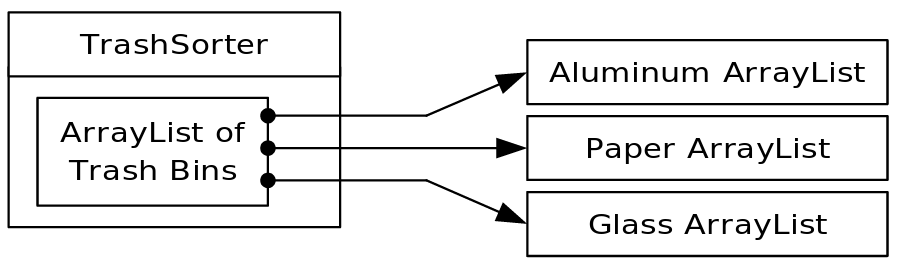
\includegraphics[width=\textwidth]{Pag147SinTraducir.png}

La inicialización de objetos \textbf{TrashSorter} ahora debe ser cambiado cada vez que un nuevo tipo de \textbf{Trash} se añade al modelo. Usted podría imaginar que la clase \textbf{TrashSorter} podría ser algo como esto:     \newline

\begin{lstlisting} 
class TrashSorter(ArrayList): 
  def sort(self, Trash t): /* ... */  
\end{lstlisting}

Es decir, \textbf{TrashSorter} es un \textbf{ArrayList} de referencias a \textbf{ArrayList}s de referencias \textbf{Trash}, y con \textbf{add()} se puede instalar otro, así:  \newline

\begin{lstlisting} 
TrashSorter ts = TrashSorter() 
ts.add(ArrayList()) 
\end{lstlisting}

Ahora, sin embargo, \textbf{sort( )} se convierte en un problema. ¿Cómo el método estático - codificado trata con el hecho de que un nuevo tipo ha sido añadido? Para solucionar esto, la información de tipo debe ser removido de \textbf{sort( )} de manera que todo lo que necesita hacer es llamar a un método genérico que se ocupa de los detalles de tipo. Esto, por supuesto, es otra manera de describir un método dinámicamente enlazado. Así \textbf{sort( )} simplemente se moverá a través de la secuencia y llamará a un método dinámicamente enlazado para cada \textbf{ArrayList}. Dado que el trabajo de este método es tomar las piezas de \textbf{Trash} en que está interesado, este es llamado \textbf{grab(Trash)}. La estructura ahora queda como:       \newline

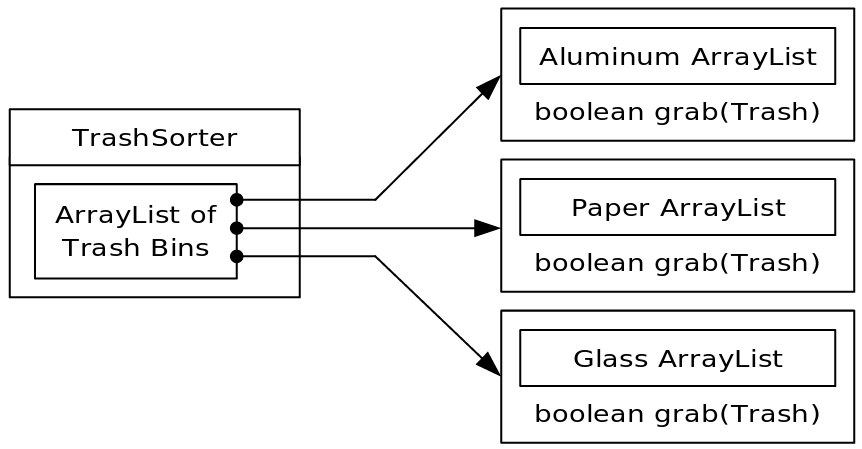
\includegraphics[width=\textwidth]{Pagina148SinTraducir.png}

\textbf{TrashSorter} necesita llamar cada método \textbf{grab()} y obtener un resultado diferente dependiendo de qué tipo de \textbf{Trash} \textbf{ArrayList} actual está sosteniendo. Es decir, cada \textbf{ArrayList} debe ser consciente del tipo que contiene. El enfoque clásico a este problema es crear una clase "\textbf{Trash bin} : Contenedor de basura" base y heredar una nueva clase derivada para cada tipo diferente que quiera mantener. Si Java tenía un mecanismo de tipo parametrizado ese probablemente sería el enfoque más sencillo. Pero en lugar de la codificación manual de todas las clases que tal mecanismo debe estar construyendo para nosotros, una mayor observación puede producir un mejor enfoque.   \newline

Un principio básico de diseño en programación orientada a objetos es: "Usar los miembros de datos para la variación en el estado, utilizar el polimorfismo para la variación en el comportamiento." Su primer pensamiento podría ser que el método \textbf{grab( )} ciertamente se comporta de manera diferente para un \textbf{ArrayList} que contiene \textbf{Paper} que por su parte contiene \textbf{Glass}. Pero lo que hace es estrictamente dependiente del tipo, y nada más. Esto podría interpretarse como un estado diferente, y dado que Java tiene una clase para representar el tipo \textbf{(Class)}, esto se puede utilizar para determinar el tipo de \textbf{Trash} que sostendrá a \textbf{Tbin} en particular .       \newline

El constructor para este \textbf{Tbin} requiere lo de la \textbf{Class} de su elección. Esto le dice al \textbf{ArrayList} qué tipo se supone que debe mantener. Entonces el método \textbf{grab( )} usa \textbf{Class BinType} y RTTI para ver si el objeto \textbf{Trash} que ha entregado coincide con el tipo que se supone que ha seleccionado.      \newline

Aquí esta una nueva versión del programa:       \newline

\begin{lstlisting} 
# c12:recycleb:RecycleB.py 
# Containers that grab objects of interest. 

# A container that admits only the right type 
# of Trash (established in the constructor): 
class Tbin: 
  private Collection list = ArrayList() 
  private Class type 
  def __init__(self, Class binType): type = binType  
  def grab(self, Trash t): 
    # Comparing class types: 
    if(t.getClass().equals(type)): 
      list.add(t) 
      return 1 # Object grabbed 
      
    return 0 # Object not grabbed  
    
  def iterator(self): 
    return list.iterator() 
    
class TbinList(ArrayList): 
  def sort(self, Trash t): 
    Iterator e = iterator() # Iterate over self 
    while(e.hasNext()) 
      if(((Tbin)e.next()).grab(t)) return 
    # Need a Tbin for this type: 
        add(Tbin(t.getClass())) 
    sort(t) # Recursive call 
    
class RecycleB(UnitTest): 
  Collection bin = ArrayList() 
  TbinList trashBins = TbinList() 
  def __init__(self): 
    ParseTrash.fillBin("../trash/Trash.dat",bin) 
    
  def test(self): 
    Iterator it = bin.iterator() 
    while(it.hasNext()) 
      trashBins.sort((Trash)it.next()) 
    Iterator e = trashBins.iterator() 
    while(e.hasNext()): 
      Tbin b = (Tbin)e.next() 
      Trash.sumValue(b.iterator()) 
      
    Trash.sumValue(bin.iterator()) 
    
  def main(self, String args[]): 
    RecycleB().test() 
    
# :~ 
\end{lstlisting}

\textbf{Tbin} contiene una referencia \textbf{Class} \textbf{type} que establece en el constructor qué tipo debe seleccionar. El método \textbf{grab()} revisa este tipo contra el objeto que se pasa. Tenga en cuenta que en este diseño, \textbf{grab()} solo acepta objetos \textbf{Trash} de este modo usted consigue la comprobación de tipos en tiempo de compilación del tipo base, pero también se podría aceptar solo \textbf{Object} y aún así funcionaría.      \newline

\textbf{TbinList} sostiene un conjunto de referencias \textbf{Tbin}, así que \textbf{sort()} puede iterar a través de los \textbf{Tbin}s cuando está buscando una pareja para el objeto \textbf{Trash} se lo ha transmitido. Si este no encuentra una pareja, crea un nuevo \textbf{Tbin} para el tipo que no ha sido enconstrado, y hace una llamada recursiva a sí mismo – la próxima vez encontrará el nuevo bin.
%   time around == vez

Note la generalidad de este código: no cambia en absoluto si se añaden nuevos tipos. Si la mayor parte de su código no necesita cambiar cuando se añade un nuevo tipo (o algún otro cambio ocurre) entonces usted tiene un sistema fácilmente extensible.

\newpage


\subsection*{Despacho múltiple}
\label{subsec:dmul}
\addcontentsline{toc}{subsection}{\nameref{subsec:dmul}}

El diseño anterior es ciertamente satisfactorio. La adición de nuevos tipos al sistema consiste en añadir o modificar clases distintas sin causar cambios en el código que se propaguen por todo el sistema. En adición, RTTI no está "mal utilizada" como lo estaba en \textbf{RecycleA.py}. Sin embargo, es posible ir un paso más allá y tomar un punto de vista purista sobre RTTI y decir que debe ser eliminada por completo de la operación de clasificar la basura en los contenedores. \newline

Para lograr esto, primero debe tomar la perspectiva de que todas las actividades de tipo dependiente — tal como la detección del tipo de un pedazo de \textbf{Trash} y ponerla en el recipiente apropiado — deben ser controladas a través del polimorfismo y de un enlace dinámico. \newline

Los ejemplos anteriores primero ordenados por tipo, luego actuando en las secuencias de elementos que eran todos de un tipo en particular. Pero cada vez que usted se encuentra eligiendo tipos particulares, deténgase y piense. 
Toda la idea de polimorfismo (dinámicamente enlazado con llamadas a métodos) es encargarse de la información de tipo específico para usted. Así que ¿por qué la búsqueda de tipos?      \newline

La respuesta es algo que probablemente no se piensa: que Python sólo realiza despacho individual. Es decir, si está realizando una operación en más de un objeto cuyo tipo es desconocido, Python invocará el mecanismo de enlace dinámico en sólo uno de esos tipos. Esto no resuelve el problema, así que se termina la detección de algunos tipos manualmente y produciendo eficazmente su propio comportamiento de enlace dinámico. \newline

La solución es llamada  \textit{multiple dispatching (Despacho múltiple)} lo cual significa la creación de una configuración tal que una única llamada al método produce más de una llamada a un método dinámico y por lo tanto determina más de un tipo en el proceso. Para conseguir este efecto, se necesita trabajar con más de una jerarquía de tipos: se necesitará una jerarquía de tipos para cada envío. En el siguiente ejemplo se trabaja con dos jerarquías: la familia \textbf{Trash} existente y una jerarquía de los tipos de contenedores de basura, en los cuales los desechos serán colocados. Esta segunda jerarquía no siempre es evidente y en este caso se requiere crear un orden para producir múltiples despachos (en este caso habrá sólo dos despachos, lo cual hace referencia como \textit{double dispatching (despacho doble)}).
% Despacho, envio (sinonimos)
\newpage


\subsubsection*{La implementación del despacho doble}
\label{subsubsec:liddd}
\addcontentsline{toc}{subsubsection}{\nameref{subsubsec:liddd}}


Recuerde que el polimorfismo puede ocurrir sólo a través de llamadas a métodos, así que si quiere que se produzca el despacho doble, deben existir dos llamadas a métodos: uno utilizado para determinar el tipo dentro de cada jerarquía. En la jerarquía \textbf{Trash} habrá un nuevo método llamado \textbf{addToBin()}, que toma un argumento de un array de \textbf{TypedBin}. Utiliza este array para recorrer y tratar de agregarse a sí misma al contenedor apropiado, y aquí es donde se verá el despacho doble. \newline

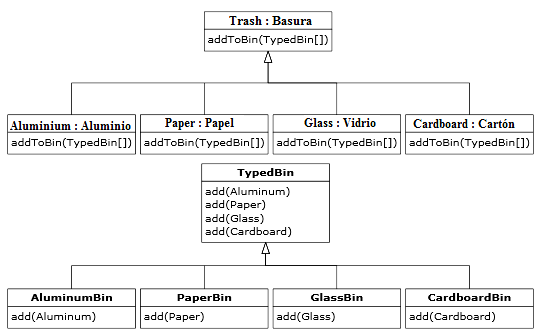
\includegraphics[width=\textwidth]{DobleDespacho}

\vspace{0.5 cm}

La nueva jerarquía es \textbf{TypedBin}, y que contiene su propio método llamado \textbf{add()} que también es utilizado polimórficamente. Pero aquí está un giro adicional: \textbf{add()} está sobrecargado  para tomar argumentos de los diferentes tipos de \textit{trash : basura}. Así que una parte esencial del esquema de doble despacho también implica una sobrecarga. El rediseño del programa produce un dilema: ahora es necesario para la clase base \textbf{Trash} contener un método \textbf{addToBin()}. Un enfoque consiste en copiar todo el código y cambiar la clase base. Otro enfoque, que puede tomar es cuando no se tiene el control del código fuente, es poner el método \textbf{addToBin( )} dentro de un \textbf{interface}, dejar \textbf{Trash} solo, y heredar nuevos tipos específicos de \textbf{Aluminum, Paper, Glass}, y \textbf{Cardboard}. Este es el enfoque que se tomará aquí.    \newline

La mayoría de las clases en este diseño debe ser \textbf{public}, por lo que se colocan en sus propios archivos. Aquí esta la interfaz:     \newline

\begin{lstlisting} 
# c12:doubledispatch:TypedBinMember.py 
# An class for adding the double  
# dispatching method to the trash hierarchy  
# without modifying the original hierarchy.

class TypedBinMember: 
  # The method: 
  boolean addToBin(TypedBin[] tb) 
# :~ 
\end{lstlisting}

En cada subtipo particular de \textbf{Aluminum, Paper, Glass} , and \textbf{Cardboard}, el método \textbf{addToBin( )} en la interfaz \textbf{interface TypedBinMember} es implementado, pero \textit{parece}  que el código es exactamente el mismo en cada caso:    \newline

\begin{lstlisting} 
# c12:doubledispatch:DDAluminum.py 
# Aluminum for double dispatching. 

class DDAluminum(Aluminum)  
    implements TypedBinMember: 
  def __init__(self, double wt): .__init__(wt)  
  def addToBin(self, TypedBin[] tb): 
    for(int i = 0 i < tb.length i++) 
      if(tb[i].add(self)) 
        return 1 
    return 0 
    
# :~ 
# c12:doubledispatch:DDPaper.py 
# Paper for double dispatching. 

class DDPaper(Paper)  
    implements TypedBinMember: 
  def __init__(self, double wt): .__init__(wt)  
  def addToBin(self, TypedBin[] tb): 
    for(int i = 0 i < tb.length i++) 
      if(tb[i].add(self)) 
        return 1 
    return 0 
    
# :~ 
# c12:doubledispatch:DDGlass.py 
# Glass for double dispatching. 

class DDGlass(Glass)  
    implements TypedBinMember: 

  def __init__(self, double wt): .__init__(wt)  
  def addToBin(self, TypedBin[] tb): 
    for(int i = 0 i < tb.length i++) 
      if(tb[i].add(self)) 
        return 1 
    return 0 
    
# :~ 
# c12:doubledispatch:DDCardboard.py 
# Cardboard for double dispatching. 

class DDCardboard(Cardboard)  
    implements TypedBinMember: 
  def __init__(self, double wt): .__init__(wt)  
  def addToBin(self, TypedBin[] tb): 
    for(int i = 0 i < tb.length i++) 
      if(tb[i].add(self)) 
        return 1 
    return 0 
    
# :~ 
\end{lstlisting}

El código en cada \textbf{addToBin( )} llama \textbf{add( )} para cada objeto \textbf{TypedBin} en el array. Pero notece el argumento: \textbf{this}. El tipo de \textbf{this} es diferente para cada subclase de \textbf{Trash}, por lo que el código es diferente. (Aunque este código se beneficiará si un mecanismo de tipo parametrizado es alguna vez agregado a Java.) Así que esta es la primera parte del doble despacho, porque una vez que está dentro de este método se sabe que es \textbf{Aluminum},  o \textbf{Paper}, etc. Durante la llamada a \textbf{add( )}, esta información se pasa a través del tipo de \textbf{this}. El compilador resuelve la llamada a la versión correcta sobrecargada de \textbf{add( )}. Pero desde que \textbf{tb[i]} produce una referencia al tipo base \textbf{TypedBin}, esta llamada va a terminar llamando a un método diferente dependiendo del tipo de \textbf{TypedBin} que está actualmente seleccionado. Ese es el segundo despacho. \newline

Aquí esta la clase base para \textbf{TypedBin}:         \newline

\begin{lstlisting} 
# c12:doubledispatch:TypedBin.py 
# A container for the second dispatch. 

class TypedBin: 
  Collection c = ArrayList() 
  def addIt(self, Trash t): 
    c.add(t) 
    return 1 
    
  def iterator(self): 
    return c.iterator() 
    
  def add(self, DDAluminum a): 
    return 0 
    
  def add(self, DDPaper a): 
    return 0 
    
  def add(self, DDGlass a): 
    return 0 
    
  def add(self, DDCardboard a): 
    return 0 
    
# :~ 
\end{lstlisting}

Se puede ver que todos los métodos sobrecargados \textbf{add( )} retornan  \textbf{false}. Si el método no está sobrecargado en una clase derivada, continuará retornando \textbf{false},  y el llamado (\textbf{addToBin( )}, en este caso)  asumirá que el objeto actual \textbf{Trash} no se ha añadido con éxito a un contenedor, y continuar buscando el contenedor correcto.         \newline

En cada una de las subclases de \textbf{TypedBin}, sólo un método sobrecargado es anulado, de acuerdo con el tipo de contenedor que está siendo creado. Por ejemplo, \textbf{CardboardBin} anula \textbf{add(DDCardboard)}. El método anulado agrega el objeto\textit{ trash : basura} a su contenedor y retorna \textbf{true}, mientras todo el resto de los métodos \textbf{add( )} en \textbf{CardboardBin} continua para devolver \textbf{false}, ya que no se han anulado. Este es otro caso en el que un mecanismo de tipo parametrizado en Java permitiría la generación automática de código. (Con C++ \textbf{template}s, no se tendría que escribir explícitamente las subclases o colocar el método \textbf{addToBin( )} en \textbf{Trash}.)      \newline

Puesto que para este ejemplo los tipos de basura se han personalizado y colocado en un directorio diferente, se necesitará un archivo de datos de basura diferente para hacer que funcione. Aquí está un posible \textbf{DDTrash.dat}:      \newline

\begin{lstlisting} 
# c12:doubledispatch:DDTrash.dat 
DDGlass:54 
DDPaper:22 
DDPaper:11 
DDGlass:17 
DDAluminum:89 
DDPaper:88 
DDAluminum:76 
DDCardboard:96 
DDAluminum:25 
DDAluminum:34 
DDGlass:11 
DDGlass:68 
DDGlass:43 
DDAluminum:27 
DDCardboard:44 
DDAluminum:18 
DDPaper:91 
DDGlass:63 
DDGlass:50 
DDGlass:80 
DDAluminum:81 
DDCardboard:12 
DDGlass:12 
DDGlass:54 
DDAluminum:36 
DDAluminum:93 
DDGlass:93 
DDPaper:80 
DDGlass:36 
DDGlass:12 
DDGlass:60 
DDPaper:66 
DDAluminum:36 
DDCardboard:22 
# :~ 
\end{lstlisting}

Aquí esta el resto del programa:        \newline

\begin{lstlisting} 
# c12:doubledispatch:DoubleDispatch.py 
# Using multiple dispatching to handle more 
# than one unknown type during a method call. 

class AluminumBin(TypedBin): 
  def add(self, DDAluminum a): 
    return addIt(a) 
    
class PaperBin(TypedBin): 
  def add(self, DDPaper a): 
    return addIt(a) 
    
class GlassBin(TypedBin): 
  def add(self, DDGlass a): 
    return addIt(a) 
    
class CardboardBin(TypedBin): 
  def add(self, DDCardboard a): 
    return addIt(a) 
    
class TrashBinSet: 
  private TypedBin[] binSet =: 
    AluminumBin(), 
    PaperBin(), 
    GlassBin(), 
    CardboardBin() 
    
  def sortIntoBins(self, Collection bin): 
    Iterator e = bin.iterator() 
    while(e.hasNext()): 
      TypedBinMember t =  
        (TypedBinMember)e.next() 
      if(!t.addToBin(binSet)) 
        System.err.println("Couldn't add " + t) 
        
  public TypedBin[] binSet(): return binSet      
  
  class DoubleDispatch(UnitTest): 
  Collection bin = ArrayList() 
  TrashBinSet bins = TrashBinSet() 
  def __init__(self): 
    # ParseTrash still works, without changes: 
    ParseTrash.fillBin("DDTrash.dat", bin) 
    
  def test(self): 
    # Sort from the master bin into  
    # the individually-typed bins: 
    bins.sortIntoBins(bin) 
    TypedBin[] tb = bins.binSet() 
    # Perform sumValue for each bin... 
    for(int i = 0 i < tb.length i++) 
      Trash.sumValue(tb[i].c.iterator()) 
    # ... and for the master bin 
    Trash.sumValue(bin.iterator()) 
    
  def main(self, String args[]): 
    DoubleDispatch().test() 
    
# :~ 
\end{lstlisting}

\textbf{TrashBinSet} encapsula todos los diferentes tipos de \textbf{ TypedBin}s, junto con el método \textbf{sortIntoBins( )}, que es donde todo el despacho doble toma lugar. Se puede ver que una vez que la estructura está configurada, la clasificación en los distintos \textbf{TypedBin}s es muy fácil. En adición, la eficiencia de dos llamadas al método dinámico es probablemente mejor que cualquier otra forma de ordenamiento. \newline

Note la facilidad de uso de este sistema en \textbf{main( )}, así como la completa independencia de cualquier información de tipo específico dentro de \textbf{main( )}. Todos los otros métodos que hablan sólo a la interfaz de la clase base \textbf{Trash} serán igualmente invulnerable a los cambios en los tipos \textbf{Trash}.         \newline

Los cambios necesarios para agregar un nuevo tipo son relativamente aislados: modificar \textbf{TypedBin}, heredar el nuevo tipo de \textbf{Trash} con su método \textbf{addToBin( )}, luego heredar un nuevo \textbf{TypedBin} (esto es realmente sólo una copia y sencilla edición), y por último añadir un nuevo tipo en la inicialización agregada de \textbf{TrashBinSet}.  \newline

\subsection*{El patrón \textit{Visitor} (Visitante)}
\label{subsec:epV}
\addcontentsline{toc}{subsection}{\nameref{subsec:epV}}

Ahora considerar la aplicación de un patrón de diseño que tiene un objetivo completamente diferente al problema de clasificación de basura. \newline

Para este patrón, ya no se debe estar preocupado con la optimización de la adición de nuevos tipos de \textbf{Trash} para el sistema. Ciertamente, este patrón hace que la adición de un nuevo tipo de \textbf{Trash} sea más complicado. El supuesto es que se tiene una jerarquía de clases primaria que es fija; quizás es de otro proveedor y no puedes realizar cambios en esa jerarquía. Sin embargo, se tenía como añadir nuevos métodos polimórficos a esa jerarquía, lo cual significa que normalmente tenía que añadir algo a la interfaz de la clase base. Así el dilema es que se necesita añadir métodos a la clase base, pero no se puede tocar la clase base. ¿Cómo se puede evitar esto?  \newline

El patrón de diseño que resuelve este tipo de problema es llamado un "visitor" (visitante) (al final en el libro \textit{Design Patterns}), y se basa en el esquema de despacho doble mostrado en la última sección. \newline

El patrón \textit{visitor : visitante} le permite extender la interfaz del tipo primario mediante la creación de una jerarquía de clases por separado de tipo \textbf{Visitor} para virtualizar las operaciones realizadas en el tipo primario. Los objetos del tipo primario simplemente "aceptan" el visitante, a continuación, llaman al método del \textit{visitor}, enlazado dinámicamente. Se ve así:       \newline

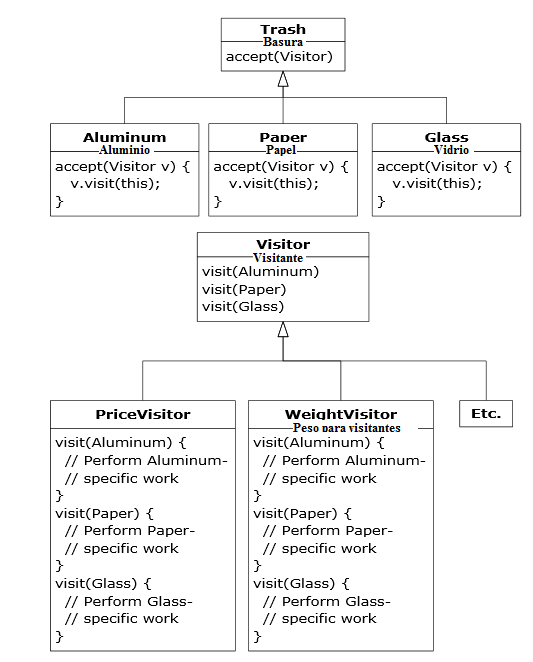
\includegraphics[width=\textwidth]{Pagna159}

Ahora, si \textbf{v} es una referencia \textbf{Visitable} para un objeto \textbf{Aluminum}, el código:    \newline

\begin{lstlisting} 
PriceVisitor pv = PriceVisitor() 
v.accept(pv) 
\end{lstlisting}

Utiliza despacho doble para causar dos llamadas a métodos polimórficos: el primero para seleccionar la versión de \textbf{Aluminum} de \textbf{accept( )}, y el segundo dentro de \textbf{accept( )} cuando la versión especifica de \textbf{visit( )} es llamada de forma dinamica usando la clase base \textbf{Visitor} con referencia \textbf{v}.         \newline

Esta configuración significa que la nueva funcionalidad puede ser añadida al sistema en forma de nuevas subclases de \textbf{Visitor}. La jerarquía \textbf{Trash} no necesita ser tocada. Este es el principal beneficio del patrón \textit{visitor}, se puede agregar nueva funcionalidad polimórfica a una jerarquía de clases sin tocar esa jerarquía (una vez que los métodos \textbf{accept( )} se han instalado). Tenga en cuenta que el beneficio es útil aquí, pero no es exactamente lo que empezamos a lograr, así que a primera vista podría decidirse que esta no es la solución deseada.      \newline

Pero mire una cosa que se ha logrado: la solución visitante Evita la clasificación de la secuencia \textbf{Trash} maestro en secuencias escritas individuales. Así, usted puede dejar todo en la única secuencia maestra y simplemente pasar a través de esa secuencia utilizando el visitante apropiado para lograr el objetivo. Aunque este comportamiento parece ser un efecto secundario del visitante, Esto proporciona lo que se requiere (evitando RTTI).       \newline

El despacho doble en el patrón \textbf{Visitor} se ocupa de determinar tanto el tipo de \textbf{Trash} como el tipo de \textbf{Visitor}. En el siguiente ejemplo, hay dos implementaciones de \textbf{Visitor: PriceVisitor} tanto para determinar y resumir el precio, y \textbf{WeightVisitor} para hacer un seguimiento de los pesos.      \newline

Se puede ver todo esto implementado en la nueva y mejorada versión del programa de reciclaje.        \newline

Al igual que con \textbf{DoubleDispatch.py}, la clase \textbf{Trash} se deja sola y una nueva interfaz es creada para agregar el método \textbf{accept( )}: \newline

\begin{lstlisting} 
# c12:trashvisitor:Visitable.py 
# An class to add visitor functionality  
# to the Trash hierarchy without  
# modifying the base class. 

class Visitable: 
  # The method: 
  def accept(self, Visitor v) 
# :~ 
\end{lstlisting}

Dado que no hay nada concreto en la clase base \textbf{Visitor}, se puede crear como una \textbf{interface}: \newline

\begin{lstlisting} 
# c12:trashvisitor:Visitor.py 
# The base class for visitors. 

class Visitor: 
  def visit(self, Aluminum a) 
  def visit(self, Paper p) 
  def visit(self, Glass g) 
  def visit(self, Cardboard c) 
# :~ 
\end{lstlisting}


\subsection*{Un decorador reflexivo}
\label{subsec:udr}
\addcontentsline{toc}{subsection}{\nameref{subsec:udr}}


En este punto, se podría seguir el mismo criterio que se utilizó para el despacho doble y crear nuevos subtipos de \textbf{Aluminum, Paper, Glass}, y \textbf{Cardboard} que implementan el método \textbf{accept( )}. Por ejemplo, el nuevo \textbf{Visitable Aluminum} se vería así: \newline

\begin{lstlisting} 
# c12:trashvisitor:VAluminum.py 
# Taking the previous approach of creating a 
# specialized Aluminum for the visitor pattern. 

class VAluminum(Aluminum)  
    implements Visitable: 
  def __init__(self, double wt): .__init__(wt)  
  def accept(self, Visitor v): 
    v.visit(self) 

# :~ 
\end{lstlisting}

Sin embargo, parece que se está enfrentando a una "explosión de interfaces:" \textbf{Trash} básico, versiones especiales para el despacho doble, y ahora las versiones más especiales para los visitantes. Claro, esta "explosión de interfaces" es arbitraria — uno podría simplemente poner los métodos adicionales de la clase \textbf{Trash}. Si se ignora que en su lugar se puede tener la oportunidad de utilizar el patrón \textit{Decorador}: parece que debería ser posible crear un \textit{Decorador} que puede ser envuelto alrededor de un objeto ordinario \textbf{Trash} y producirá la misma interfaz que \textbf{Trash} y agrega el método extra \textbf{accept( )}. De hecho, es un ejemplo perfecto del valor del \textit{Decorador}.         \newline

El doble despacho crea un problema, no obstante. Como se basa en la sobrecarga de ambos \textbf{accept( )} y \textbf{visit( )}, esto parecería requerir código especializado para cada versión diferente del método \textbf{accept( )}. Con las plantillas de C ++, esto sería bastante fácil de lograr (ya que las plantillas generan automáticamente código de tipo especializado) pero Python no tiene tal mecanismo — al menos no parece. Sin embargo, la propiedad de reflexión de Python le permite determinar la información de tipo en tiempo de ejecución, y llegar a resolver muchos problemas que parecerían requerir plantillas (aunque no tan simplemente). Aquí está el decorador que hace el truco\footnote{Esta fue una solución creada por Jaroslav Tulach en una clase de diseño de patrones que di en Praga}:       \\newpage

\begin{lstlisting} 
# c12:trashvisitor:VisitableDecorator.py 
# A decorator that adapts the generic Trash 
# classes to the visitor pattern. 
class VisitableDecorator 
extends Trash implements Visitable: 
  private Trash delegate 
  private Method dispatch 
  def __init__(self, Trash t): 
    delegate = t 
    try: 
      dispatch = Visitor.class.getMethod ( 
        "visit", Class[]: t.getClass()  
      ) 
     catch (Exception ex): 
      ex.printStackTrace() 
  def getValue(self): 
    return delegate.getValue() 
  def getWeight(self): 
    return delegate.getWeight() 
  def accept(self, Visitor v): 
    try: 
      dispatch.invoke(v, Object[]{delegate) 
     catch (Exception ex): 
      ex.printStackTrace() 
# :~ 
\end{lstlisting}

[[Descripción del uso de Reflexión]]  \newline

La única otra herramienta que necesitamos es un nuevo tipo de adaptador \textbf{Fillable} que automáticamente decora los objetos a medida que se crean a partir del archivo original \textbf{Trash.dat}. Pero esto bien podría ser un decorador de sí mismo, la decoración de cualquier tipo de \textbf{Fillable}:        \newline

\begin{lstlisting} 
# c12:trashvisitor:FillableVisitor.py  
# Adapter Decorator that adds the visitable  
# decorator as the Trash objects are  
# being created. 

class FillableVisitor 
implements Fillable: 
  private Fillable f 
  def __init__(self, Fillable ff): f = ff  
  def addTrash(self, Trash t): 
    f.addTrash(VisitableDecorator(t)) 
# :~ 
\end{lstlisting}
Ahora se puede envolver alrededor de cualquier tipo de \textbf{Fillable} existente,  o cualquier otros nuevos que aún no se han creado. \newline

El resto del programa crea tipos \textbf{Visitor} específicos y los envía a través de una lista única de objetos \textbf{Trash}:   \newline

\begin{lstlisting} 
# c12:trashvisitor:TrashVisitor.py  
# The "visitor" pattern with VisitableDecorators. 

# Specific group of algorithms packaged 
# in each implementation of Visitor: 
class PriceVisitor(Visitor): 
  private double alSum # Aluminum 
  private double pSum # Paper 
  private double gSum # Glass 
  private double cSum # Cardboard 
  def visit(self, Aluminum al): 
    double v = al.getWeight() * al.getValue() 
    print "value of Aluminum= " + v 
    alSum += v 
    
  def visit(self, Paper p): 
    double v = p.getWeight() * p.getValue() 
    print "value of Paper= " + v 
    pSum += v 
    
  def visit(self, Glass g): 
    double v = g.getWeight() * g.getValue() 
    print "value of Glass= " + v 
    gSum += v 
    
  def visit(self, Cardboard c): 
    double v = c.getWeight() * c.getValue() 
    print "value of Cardboard = " + v 
    cSum += v 
    
  def total(self): 
    print ( 
      "Total Aluminum: $" + alSum + 
      "\n Total Paper: $" + pSum +  
      "\nTotal Glass: $" + gSum +  
      "\nTotal Cardboard: $" + cSum + 
      "\nTotal: $" +  
        (alSum + pSum + gSum + cSum)) 
        
class WeightVisitor(Visitor): 
  private double alSum # Aluminum 
  private double pSum # Paper 
  private double gSum # Glass 
  private double cSum # Cardboard 
  
  def visit(self, Aluminum al): 
    alSum += al.getWeight() 
    print ("weight of Aluminum = " 
        + al.getWeight()) 
        
  def visit(self, Paper p): 
    pSum += p.getWeight() 
    print ("weight of Paper = " 
        + p.getWeight()) 
        
  def visit(self, Glass g): 
    gSum += g.getWeight() 
    print ("weight of Glass = " 
        + g.getWeight()) 
        
  def visit(self, Cardboard c): 
    cSum += c.getWeight() 
    print ("weight of Cardboard = " 
        + c.getWeight()) 
        
  def total(self): 
    print ( 
      "Total weight Aluminum: "  + alSum + 
      "\nTotal weight Paper: " + pSum + 
      "\nTotal weight Glass: " + gSum + 
      "\nTotal weight Cardboard: " + cSum + 
      "\nTotal weight: " +  
        (alSum + pSum + gSum + cSum))
        
class TrashVisitor(UnitTest): 
  Collection bin = ArrayList() 
  PriceVisitor pv = PriceVisitor() 
  WeightVisitor wv = WeightVisitor() 
  def __init__(self): 
    ParseTrash.fillBin("../trash/Trash.dat",  
      FillableVisitor( 
        FillableCollection(bin))) 
        
  def test(self): 
    Iterator it = bin.iterator() 
    while(it.hasNext()): 
      Visitable v = (Visitable)it.next() 
      v.accept(pv) 
      v.accept(wv) 
      
    pv.total() 
    wv.total() 
    
  def main(self, String args[]): 
    TrashVisitor().test() 
    
# :~ 
\end{lstlisting}

En \textbf{Test( )}, se observa cómo se añade la visitabilidad simplemente creando un tipo diferente de contenedor usando el decorador. Se observa también que el adaptador \textbf{FillableCollection} tiene la apariencia de ser utilizado como decorador (para \textbf{ArrayList}) en esta situación.  Ahora bien, cambia completamente la interfaz del \textbf{ArrayList}, visto que la definición de \textit{Decorador} es que la interfaz de la clase decorada aún debe estar allí después de la decoración.      \newline

Tenga en cuenta que la forma del código del cliente (que se muestra en la clase \textbf{Test}) ha cambiado de nuevo, a partir de los enfoques originales al problema. Ahora sólo hay un solo contenedor \textbf{Trash}. Los dos objetos \textbf{Visitor} son aceptados en cada elemento de la secuencia, y realizan sus operaciones. Los visitantes mantienen sus propios datos internos para concordar los pesos y los precios totales.        \newline

Finalmente, allí no hay identificación de tipo en tiempo de ejecución que no sea emitido a \textbf{Trash} cuando se sacan cosas fuera de la secuencia. Esto, también, podría ser eliminado con la implementación de tipos parametrizados en Java.        \newline

Una manera de distinguir esta solución de la solución de despacho doble descrita anteriormente, es tener en cuenta que, en la solución del doble despacho, solamente uno de los métodos sobrecargados, \textbf{add( )},  fue anulado cuando se creó cada subclase, mientras que aquí cada uno de los métodos \textbf{visit( )} sobrecargados es anulado en cada subclase de \textbf{Visitor}.          \newline

\subsubsection*{¿Más acoplamiento?}
\label{subsubsec:moreA}
\addcontentsline{toc}{subsubsection}{\nameref{subsubsec:moreA}}


Hay mucho más código aquí, y hay acoplamiento definitivo entre la jerarquía \textbf{Trash} y la jerarquía \textbf{Visitor}. Ahora bien, también hay alta cohesión dentro de los respectivos conjuntos de clases: cada uno de ellos hacen una sola cosa (\textbf{Trash} describe Basura, mientras que \textbf{Visitor} describe las acciones realizadas en \textbf{Trash}), que es un indicador de un buen diseño. Claro, en este caso funciona bien sólo si está agregando nuevos \textbf{Visitor}s, pero esto se obtiene en el camino cuando se agregan nuevos tipos de \textbf{Trash}.          \newline

Bajo acoplamiento entre clases y alta cohesión dentro de una clase es sin duda un objetivo de diseño importante. Aplicado sin pensar, sin embargo, puede impedirle el logro de un diseño más elegante. Parece que algunas clases, inevitablemente, tienen una cierta intimidad entre ellas. Estos a menudo ocurren en parejas que quizás podrían ser llamados \textit{couplets : coplas}; por ejemplo, los contenedores y los iteradores. El par anterior \textbf{Trash-Visitor} parece ser otro de tipo \textit{couplet}.    \newline

\subsection*{¿RTTI considerado dañino?}
\label{subsec:rtticd}
\addcontentsline{toc}{subsection}{\nameref{subsec:rtticd}}

Varios diseños en este capítulo intentan eliminar RTTI, lo cual podría darle la impresión de que se “considera perjudicial" (la condena utilizado para pobres, el malogrado \textbf{goto}, que por lo tanto nunca fue puesto en Java). Esto no es verdad; es el mal uso de RTTI, ese es el problema. La razón por la que nuestros diseños eliminan RTTI se debe a la mala aplicación de esa característica que impide extensibilidad, mientras que el objetivo expresado era poder añadir un nuevo tipo al sistema con el menor impacto alrededor del código como sea posible. Dado que RTTI es a menudo mal usado por tener que buscar cada tipo en su sistema, provoca que el código que no sea extensible: cuando se agrega un nuevo tipo, se tiene que ir a buscar por todo el código en el que se usa RTTI, y si se pierde alguno, no se conseguirá ayuda del compilador.     \newline

Sin embargo, RTTI no crea automáticamente el código no extensible. Vamos a revisar el reciclador de basura una vez más. Esta vez, una nueva herramienta será introducida, la cual yo llamo un \textbf{TypeMap}. Este contiene un \textbf{HashMap} que contiene \textbf{ArrayList}s, pero la interfaz es simple: se puede agregar \textbf{add( )} como un nuevo objeto, y \textbf{get( )} como un \textbf{ArrayList} que contiene todos los objetos de un tipo particular. Las claves para el contenido \textbf{HashMap} son los tipos en el \textbf{ArrayList} asociado. La belleza de este diseño (sugerido por Larry O'Brien) es que el \textbf{TypeMap} agrega dinámicamente un nuevo par cada vez que encuentra un nuevo tipo, por lo que cada vez que añade un nuevo tipo al sistema (incluso si se agrega el nuevo tipo en tiempo de ejecución), se adapta.  \newline

Nuestro ejemplo  nuevamente se basará en la estructura de los tipos \textbf{Trash} en \textbf{package c12.Trash} (y el archivo \textbf{Trash.dat} utilizado se pueden utilizar aquí sin modificar):        \newline

\begin{lstlisting} 
# c12:dynatrash:DynaTrash.py  
# Using a Map of Lists and RTTI 
# to automatically sort trash into 
# ArrayLists. This solution, despite the 
# use of RTTI, is extensible. 

# Generic TypeMap works in any situation: 
class TypeMap: 
  private Map t = HashMap() 
  def add(self, Object o): 
    Class type = o.getClass() 
    if(t.has_key(type)) 
      ((List)t.get(type)).add(o) 
    else: 
      List v = ArrayList() 
      v.add(o) 
      t.put(type,v) 
      
  def get(self, Class type): 
    return (List)t.get(type) 
    
  def keys(self):  
    return t.keySet().iterator()  
    
# Adapter class to allow callbacks 
# from ParseTrash.fillBin(): 
class TypeMapAdapter(Fillable): 
  TypeMap map 
  def __init__(self, TypeMap tm): map = tm  
  def addTrash(self, Trash t): map.add(t)  
  
class DynaTrash(UnitTest): 
  TypeMap bin = TypeMap() 
  
    def __init__(self): 
    ParseTrash.fillBin("../trash/Trash.dat",  
      TypeMapAdapter(bin)) 
      
  def test(self): 
    Iterator keys = bin.keys() 
    while(keys.hasNext()) 
      Trash.sumValue( 
        bin.get((Class)keys.next()).iterator())
        
  def main(self, String args[]): 
    DynaTrash().test() 
# :~ 
\end{lstlisting}

Aunque potente, la definición para \textbf{TypeMap} es simple. Contiene un \textbf{HashMap}, y el método \textbf{add( )} hace la mayoría del trabajo. Cuando se agrega un nuevo objeto \textbf{add( )}, se extrae la referencia para el objeto \textbf{Class} para ese tipo. Esto se utiliza como una clave para determinar si un \textbf{ArrayList} que sostiene objetos de ese tipo ya está presente en el \textbf{HashMap}. Si es así, ese \textbf{ArrayList} se extrae y el objeto se añade al \textbf{ArrayList}. Si no, el objeto \textbf{Class} y un nuevo \textbf{ArrayList} se añaden como un par clave-valor.       \newline

Se puede obtener un \textbf{Iterator} de todos los objetos \textbf{Class} de   \textbf{keys( )}, y usar cada objeto \textbf{Class} para buscar el correspondiente \textbf{ArrayList} con \textbf{get( )}. Y eso es todo lo que hay que hacer.         \newline

El método \textbf{filler( )} es interesante porque se aprovecha del diseño de \textbf{ParseTrash.fillBin( )},  que no sólo tratar de llenar un \textbf{ArrayList} sino cualquier cosa que implementa la interfaz \textbf{Fillable} con su método \textbf{addTrash( )}.  Todo \textbf{filler( )} necesita hacer es devolver una referencia a una \textbf{interface} que implementa \textbf{Fillable}, y luego esta referencia puede ser utilizado como un argumento a \textbf{fillBin( )} como esto:    \newline

\begin{lstlisting} 
ParseTrash.fillBin("Trash.dat", bin.filler()) 
\end{lstlisting}

Para producir esta referencia, una \textit{clase interna anónima} (descrito en el capítulo 8 de \textit{Thinking in Java}, segunda edición) es utilizada. Nunca se necesita un llamado a la clase para implementar \textbf{Fillable}, sólo necesita una referencia a un objeto de esa clase, por lo que este es un uso apropiado de las clases internas anónimas. \newline

Una cosa interesante sobre este diseño es que a pesar de que no fue creado para manejar la clasificación, \textbf{fillBin( )} está realizando una clasificación cada vez que se inserta un objeto \textbf{Trash} dentro de \textbf{bin}.        \newline

Gran parte de \textbf{class DynaTrash} debería estar familiarizado a partir de los ejemplos anteriores. Esta vez, en lugar de colocar los nuevos objetos \textbf{Trash} en un \textbf{bin} de tipo \textbf{ArrayList}, \textbf{bin} es de tipo \textbf{TypeMap}, así que cuando la basura es arrojada en \textbf{bin} se ordena de inmediato por el \textbf{TypeMap} del mecanismo de clasificación interna. Dando un paso a través de \textbf{TypeMap} y operando en cada \textbf{ArrayList} individual se convierte en un asunto sencillo.  \newline

Como puede ver, la adición de un nuevo tipo al sistema no afectará este código en absoluto, y el código en \textbf{TypeMap} es completamente independiente. Esta es ciertamente la solución más pequeña del problema, y podría decirse que el más elegante también. No depende mucho de de RTTI, pero observe que cada par clave-valor en el \textbf{HashMap} está en busca de un solo tipo. En adición, no hay manera que se pueda "olvidar" añadir el código adecuado a este sistema cuando se agrega un nuevo tipo, ya que no hay ningún código que necesite agregar.       \newline

\subsection*{Resumen}
\label{subsec:Resumen}
\addcontentsline{toc}{subsection}{\nameref{subsec:Resumen}}

Surgir %aparecer, subir
con un diseño como \textbf{TrashVisitor.py} que contiene una gran cantidad de código que los diseños anteriores puede parecer en un principio ser contraproducente. Vale la pena notar lo que estás tratando de lograr con varios diseños. Los patrones de diseño en general se esfuerzan por \textit{separar las cosas que cambian de las cosas que permanecen igual}. Las "cosas que cambian" puede referirse a muchos tipos diferentes de cambios. Quizás el cambio ocurre porque el programa se coloca en un nuevo entorno o porque algo en el entorno actual cambia: (esto podría ser: "El usuario quiere añadir una nueva forma para el diagrama actualmente en la pantalla"). O, como en este caso, el cambio podría ser la evolución del cuerpo del código. Mientras que las versiones anteriores del ejemplo de clasificación de basura enfatizaron la adición de nuevos tipos de \textbf{Trash} al sistema, \textbf{TrashVisitor.py} le permite añadir fácilmente nuevas funcionalidades sin molestar a la jerarquía \textbf{Trash}. Hay más código en \textbf{TrashVisitor.py}, pero la adición de nueva funcionalidad para \textbf{Visitor} es de mal gusto. Si esto es algo que sucede a menudo, entonces vale la pena el esfuerzo extra y el código para hacer que suceda con más facilidad. \newline

El descubrimiento del vector de cambio no es un asunto trivial; esto no es algo que un analista usualmente puede detectar cuando el programa esté en la etapa del diseño inicial. La información necesaria probablemente no aparecerá hasta las últimas fases del proyecto: a veces sólo en las fases de diseño o de implementación se descubre una necesidad más profunda o más sutil en su sistema. En el caso de la adición de nuevos tipos (el cual fue el foco de la mayoría de los ejemplos "reciclar") se puede dar cuenta de que se necesita una jerarquía de herencia particular sólo cuando se está en la fase de mantenimiento y de inicio en la ampliación del sistema! \newline

Una de las cosas más importantes que aprenderá mediante el estudio de los patrones de diseño parece ser  un cambio de actitud de lo que se ha promovido hasta ahora en este libro. Es decir: "Programación Orientada a Objetos es todo acerca de polimorfismo." Esta declaración puede producir el síndrome "dos años meceando, con un martillo"  (todo se ve como un clavo). Dicho de otra manera, es bastante difícil "obtener" polimorfismo, y una vez que lo hace, trate de emitir  % ==moldear== cast
todos sus diseños en un molde particular.\newline

¿Qué patrones de diseño dicen que la Programación Orientada a Objetos no se trata sólo de polimorfismo?. Esto se trata de "la separación de cosas que cambian y de las cosas que permanecen igual." El Polimorfismo es una manera especialmente importante para hacer esto, y resulta ser útil si el lenguaje de programación apoya directamente el polimorfismo (por lo que no se tienen que conectar por el programador, lo que lo haría prohibitivamente caro). Pero los patrones de diseño en general muestran otras maneras de lograr el objetivo básico, y una vez que se ha entendido esto, comenzarán a surgir diseños más creativos.\newline

Desde que el libro \textit{Design Patterns} salió e hizó tal impacto, la gente ha estado buscando otros patrones. Se puede ver más de ellos aparecer con el paso del tiempo. Estos son algunos sitios recomendados por by Jim Coplien, de fama C ++ (\textit{http://www.bell-labs.com/~cope}), que es uno de los principales promotores del movimiento de los patrones:      \newline

\textit{http://st-www.cs.uiuc.edu/users/patterns \newline
http://c2.com/cgi/wiki \newline
http://c2.com/ppr  \newline
http://www.bell-labs.com/people/co \newline
pe/Patterns/Process/index.html  \newline
http://www.bell-labs.com/cgi-user/OrgPatterns/OrgPatterns  \newline
http://st-www.cs.uiuc.edu/cgi-bin/wikic/wikic  \newline
http://www.cs.wustl.edu/~schmidt/patterns.html  \newline
http://www.espinc.com/patterns/overview.html } \newline

También tenga en cuenta que ha habido una conferencia anual sobre los patrones de diseño, llamada PLOP, que produce unas actas publicadas, la tercera de las cuales salieron a finales de 1997 (todas publicadas por Addison-Wesley).   \newline

\subsection*{Ejercicios}
\label{subsec:Ejercicios14}
\addcontentsline{toc}{subsection}{\nameref{subsec:Ejercicios14}}

\begin{enumerate}
    
    \item Añadir la clase \textbf{Plastic} a \textbf{TrashVisitor.py}
    \item Agregar la clase \textbf{Plastic} a \textbf{DynaTrash.py}
    \item Crear un decorador como \textbf{VisitableDecorator}, pero para el ejemplo de despacho múltiple, junto con una clase "decorador adaptador " como la creada para \textbf{VisitableDecorator}. Construir el resto del ejemplo y demostrar que funciona.
    
\end{enumerate}           %  12 : Patrón Refactorización

\section*{13 : Proyectos}
\label{sec:proy}
\addcontentsline{toc}{section}{\nameref{sec:proy}}

%\textcolor{red}{Este capítulo no ha tenido traducción significativa todavía.}    \newline% COLOCAR COLOR ROJO

Una serie de proyectos más desafiantes para que usted pueda resolver. \newline
[[Algunos de estos pueden convertirse en ejemplos en el libro, por lo que en algún momento podría desaparecer de aquí]]


\subsection*{Ratas y Laberintos}
\label{subsec:ratas}
\addcontentsline{toc}{subsection}{\nameref{subsec:ratas}}

Primero, crea un \textit{Blackboard }\newline(citar esta referencia) que es un objeto sobre el que cualquier persona puede registrar la información. Este Blackboard particular  dibuja un laberinto, y es usado como información que vuelve sobre la estructura de un laberinto desde  las ratas que lo están  buscando. \newline

Ahora cree el propio laberinto. Como un laberinto real, este objeto revela muy poca información sobre si mismo \-dada una coordenada, que le dirá si hay paredes o espacios en las cuatro direcciones  inmediatamente que coordinan, pero no más.  Para empezar, lea el laberinto desde un archivo de texto pero considere la busqueda en internet para un algoritmo que genere un laberinto. En cualquier caso, el resultado debe ser un objeto que, dado una coordenada del laberinto, informará paredes y espacios alrededor de esa coordenada. Además, debe ser capaz de preguntar por un punto de entrada al laberinto.  \newline

Finalmente, crear la clase \textbf{Rat} laberinto-buscar. Cada rata puede comunicarse tanto con el Blackboard para dar la información actual y el laberinto para solicitar neva información sobre la base de la posición actual de la rata. Sin embargo, cada vez que una rata llega a un punto de decisión donde se ramifica el laberinto, crea una nueva rata que baja por cada una de las ramas. Cada rata es conducida por su propio hilo.   Cuando una rata llega a un callejón sin salida, termina en sí después de informar los resultados de su búsqueda final al Blackboard.\newline

El objetivo es trazar un mapa completo del laberinto, pero también usted debe determinar si la condición final será encontrada naturalmente o si el blackboard debe ser responsable de la decisión. \newline

Un ejemplo de implementación de Jeremy Meyer:    \newline

\begin{lstlisting}
# c13:Maze.py 

class Maze(Canvas): 
  private Vector lines # a line is a char array 
  private int width = -1 
  private int height = -1 
  public static void main (String [] args)  
  throws IOException: 
    if (args.length < 1): 
      print ``Enter filename" 
      System.exit(0) 
      
    Maze m = Maze() 
    m.load(args[0]) 
    Frame f = Frame() 
    f.setSize(m.width*20, m.height*20) 
    f.add(m)      
    Rat r = Rat(m, 0, 0) 
    f.setVisible(1) 
    
  def __init__(self): 
    lines = Vector() 
    setBackground(Color.lightGray) 
    
  synchronized public boolean  
  isEmptyXY(int x, int y): 
    if (x < 0) x += width 
    if (y < 0) y += height  
    # Use mod arithmetic to bring rat in line: 
    byte[] by =  
      (byte[])(lines.elementAt(y%height))   
    return by[x%width]==' ' 
    
  synchronized public void  
  setXY(int x, int y, byte newByte): 
    if (x < 0) x += width 
    if (y < 0) y += height  
    byte[] by =  
      (byte[])(lines.elementAt(y%height)) 
    by[x%width] = newByte 
    repaint() 
    
  public void  
  load(String filename) throws IOException: 
    String currentLine = null 
    BufferedReader br = BufferedReader( 
      FileReader(filename)) 
    for(currentLine = br.readLine()  
        currentLine != null 
        currentLine = br.readLine()) : 
      lines.addElement(currentLine.getBytes())        
      if(width < 0 ||  
         currentLine.getBytes().length > width) 
        width = currentLine.getBytes().length 
        
    height = len(lines) 
    br.close() 
    
  def update(self, Graphics g): paint(g)  
  public void paint (Graphics g): 
    int canvasHeight = self.getBounds().height 
    int canvasWidth  = self.getBounds().width 
    if (height < 1 || width < 1)  
      return # nothing to do  
    int width =  
      ((byte[])(lines.elementAt(0))).length 
    for (int y = 0 y < len(lines) y++): 
      byte[] b 
      b = (byte[])(lines.elementAt(y)) 
      for (int x = 0 x < width x++): 
        switch(b[x]): 
          case ' ': # empty part of maze 
            g.setColor(Color.lightGray) 
            g.fillRect( 
              x*(canvasWidth/width), 
              y*(canvasHeight/height), 
              canvasWidth/width, 
              canvasHeight/height) 
            break 
          case '*':     # a wall  
            g.setColor(Color.darkGray) 
            g.fillRect( 
              x*(canvasWidth/width), 
              y*(canvasHeight/height), 
              (canvasWidth/width)-1, 
              (canvasHeight/height)-1) 
            break 
          default:      # must be rat 
            g.setColor(Color.red) 
            g.fillOval(x*(canvasWidth/width), 
            y*(canvasHeight/height), 
            canvasWidth/width, 
            canvasHeight/height) 
            break              
            
# :~ 
# c13:Rat.py 

class Rat: 
  static int ratCount = 0 
  private Maze prison 
  private int vertDir = 0  
  private int horizDir = 0 
  private int x,y 
  private int myRatNo = 0 
  def __init__(self, Maze maze, int xStart, int 
yStart): 
    myRatNo = ratCount++ 
    print ("Rat no." + myRatNo +  
      " ready to scurry.") 
    prison = maze 
    x = xStart 
    y = yStart 
    prison.setXY(x,y, (byte)'R') 
    Thread(): 
      def run(self){ scurry()  
    .start() 
    
  def scurry(self): 
    # Try and maintain direction if possible. 
    # Horizontal backward 
    boolean ratCanMove = 1 
    while(ratCanMove): 
      ratCanMove = 0 
      
      # South  
      if (prison.isEmptyXY(x, y + 1)): 
        vertDir = 1 horizDir = 0          
        ratCanMove = 1
        
      # North 
      if (prison.isEmptyXY(x, y - 1)) 
        if (ratCanMove) 
          Rat(prison, x, y-1) 
          # Rat can move already, so give  
          # this choice to the next rat. 
        else: 
          vertDir = -1 horizDir = 0          
          ratCanMove = 1 
          
      # West 
      if (prison.isEmptyXY(x-1, y)) 
        if (ratCanMove) 
          Rat(prison, x-1, y)    
          # Rat can move already, so give  
          # this choice to the next rat. 
        else: 
          vertDir = 0 horizDir = -1          
          ratCanMove = 1 
          
      # East 
      if (prison.isEmptyXY(x+1, y)) 
        if (ratCanMove) 
          Rat(prison, x+1, y)    
          # Rat can move already, so give  
          # this choice to the next rat. 
        else: 
          vertDir = 0 horizDir = 1          
          ratCanMove = 1 
          
      if (ratCanMove): # Move original rat. 
        x += horizDir 
        y += vertDir 
        prison.setXY(x,y,(byte)'R') 
        # If not then the rat will die. 
      try: 
        Thread.sleep(2000)    
       catch(InterruptedException ie): 
       
    print ("Rat no." + myRatNo +  
      " can't move..dying..aarrgggh.") 
      
# :~     
    
\end{lstlisting}

El archivo de inicialización de laberinto:

%% AGREGAndo IMAGEN
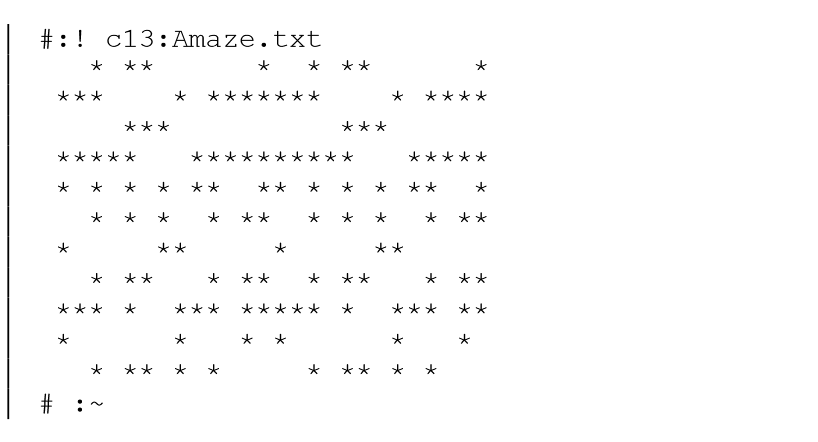
\includegraphics[width=\textwidth]{ultimaimagenTIP}


\subsubsection*{Otros Recursos para Laberinto}
\label{subsubsec:orpl}
\addcontentsline{toc}{subsubsection}{\nameref{subsubsec:orpl}}


Una discusión de algoritmos para crear laberintos así como el código fuente de Java para implementarlas : \newline

\textcolor[rgb]{0.2,0.5,0.7}{\underline{http://www.mazeworks.com/mazegen/mazegen.htm}} \newline      % COLOR AZUL

Una discusión de algoritmos para la detección de colisiones y otros comportamientos de movimiento individual/grupal de los objetos físicos autónomos: \newline

\textcolor[rgb]{0.2,0.5,0.7}{\underline{http://www.red3d.com/cwr/steer/}}


\subsubsection*{Decorador XML}
\label{subsubsec:dxml}
\addcontentsline{toc}{subsubsection}{\nameref{subsubsec:dxml}}


Crear un par de decoradores para I/O Los lectores y escritores que codifican (para el decorador Escritor) y decodificación XML.         %  13 : Proyectos

\end{document}



% \usepackage{hyperref}
%   para colocar hipervinculos
%\href{url}{http://www.texample.net/tikz/resources/}

%   Above = antedicho, encima, arriba, encima de

% He aquí todos los caracteres que tienen una función especial en 
$ 	# 	% 	& 	^ 	_ 	{ 	} 	~ 	\

%Si queremos que aparezcan como simples símbolos en el texto compilado, hemos de escribir \$ 	\# 	\% 	\& 	\^ 	\_ 	\{ 	\} 	\~ 	\textbackslash

%  \textbackslash  = \

%la funcion \textbf{} coloca el texto en negrilla

% " " \textit{} coloca cursivas

\begin{comment}
%-------------- ENUMERACION

\begin{itemize}
    \item[$*$] Madrid.
    \item Castilla la Mancha.
    \item Castilla y León.
    \begin{itemize}
        \item Segovia.
        \item Ávila.
    \end{itemize}
\end{itemize}
___________________________________

\begin{enumerate}[1.]
    \item Manzanas.
    \item Plátanos.
    \item Pescado fresco.
    \begin{enumerate}[a)]
        \item Emperador.
        \item Gallo.
    \end{enumerate}
\end{enumerate}

__________________________________-

\begin{description}
    \item[Australia:] Canguro.
    \item[EEUU:] Águila calva.
    \item[España:] Toro.
    \item[México:] Águila real.
\end{description}

\end{comment}


%% \footnote{}  pie de pagina

%  \includegraphics[width=\textwidth]{ //NOMBRE DE LA IMAGEN }   == linea para añadir imagenes gracias a la librería.

% "  " \par aplica Sangría

%  \textcolor{red}{Hola} == coloca el texto en color.


% "en el mundo del código abierto, la vergüenza es uno de los principales factores de motivación hacia el aumento de la calidad de su código!)" página 34